\documentclass[11pt]{article}

% -------------------------------
% Paquetes
% -------------------------------
\usepackage[spanish]{babel}
\usepackage[utf8]{inputenc}
\usepackage{amsmath, amssymb}
\usepackage{graphicx}
\usepackage{booktabs}
\usepackage{geometry}
\usepackage[hypertexnames=false]{hyperref}
\usepackage{float}
\usepackage{subcaption}
\usepackage{fancyhdr}

\renewcommand{\thesubfigure}{\thefigure.\arabic{subfigure}}
\makeatletter
\renewcommand\p@subfigure{}
\makeatother
\DeclareCaptionLabelFormat{figurasub}{Figura~#2}
\captionsetup[subfigure]{labelformat=figurasub,labelsep=period}
\captionsetup[figure]{labelsep=period}

\graphicspath{{figures/}}

\geometry{margin=2.5cm}

\setlength{\parindent}{0pt}
\setlength{\parskip}{6pt}
\setlength{\headheight}{42pt}
\setlength{\headsep}{18pt}

\newcommand{\reportheader}{%
\begin{minipage}{\textwidth}
\vspace{6pt}
\makebox[\textwidth][s]{Trabajo Práctico N.º~1\hfill Series de Tiempo}
\vspace{6pt}
\hrule height 0.4pt
\end{minipage}%
}

\fancypagestyle{prismstyle}{%
  \fancyhf{}
  \fancyhead[C]{\reportheader}
  \fancyfoot[C]{\thepage}
  \renewcommand{\headrulewidth}{0pt}
  \renewcommand{\footrulewidth}{0pt}
}

\fancypagestyle{plain}{%
  \fancyhf{}
  \fancyhead[C]{\reportheader}
  \fancyfoot[C]{\thepage}
  \renewcommand{\headrulewidth}{0pt}
  \renewcommand{\footrulewidth}{0pt}
}

\pagestyle{prismstyle}

% -------------------------------
% Título
% -------------------------------
\title{%
\textbf{Metodología Box-Jenkins aplicada a series con y sin desestacionalización} \\
\large Trabajo Práctico N° 1 - Series de Tiempo
}

\author{
Maestría en Economía Aplicada \\
Facultad de Ciencias Económicas - UBA \\
\\
Integrantes: \\
Christian Arias \\
Leonardo Ávila \\
Andrea Chasi \\
Julián Delgadillo \\
\\
Docente: \\
Julio Eduardo Fabris
}

\date{Fecha de entrega: 27 de abril de 2026}

\begin{document}

\maketitle

% -------------------------------
% Resumen
% -------------------------------
\begin{abstract}
El presente trabajo analiza el desempeño de distintos métodos de pronóstico aplicados a series temporales de cuentas nacionales, específicamente PIB, consumo privado, inversión bruta fija y exportaciones. Se comparan modelos estimados sobre series originales con componentes estacionales explícitos y modelos aplicados a series desestacionalizadas mediante el algoritmo X-13. Los resultados permiten evaluar empíricamente cuál estrategia de modelización presenta mayor capacidad predictiva en cada caso.
\end{abstract}

% -------------------------------
% 1. Introducción
% -------------------------------
\section{Introducción}

El análisis y pronóstico de series temporales constituye una herramienta central en economía aplicada, en particular para comprender la dinámica de variables macroeconómicas y para apoyar decisiones de política económica, planeamiento y seguimiento coyuntural. En ese marco, la capacidad de anticipar con precisión la evolución de agregados relevantes resulta especialmente valiosa cuando las series exhiben patrones de persistencia, ciclos y estacionalidad.

El presente trabajo se propone modelizar y evaluar la capacidad predictiva de distintas especificaciones econométricas aplicadas a cuatro series trimestrales de cuentas nacionales expresadas en diferencias logarítmicas: consumo privado (DL\_CPRIV), exportaciones (DL\_EXPO), inversión bruta fija (DL\_IBF) y producto interno bruto (DL\_PIB). El período analizado abarca desde 2004 hasta 2025, y la muestra se divide en un tramo de estimación (2004–2023) y un tramo de evaluación fuera de muestra (2024–2025), de modo de replicar un ejercicio de pronóstico genuino.

La pregunta de investigación que guía el trabajo es si la estacionalidad debe ser modelizada de manera directa dentro del modelo de pronóstico o si, alternativamente, conviene removerla previamente para estimar la dinámica sobre una serie ajustada. En otros términos, se busca determinar cuál de estas estrategias ofrece un mejor desempeño predictivo para series macroeconómicas trimestrales con características heterogéneas en términos de volatilidad, persistencia y estacionalidad.

Con ese objetivo se comparan dos enfoques complementarios. En primer lugar, se estiman modelos SARIMA sobre las series originales, incorporando explícitamente la estructura estacional. En segundo lugar, se implementa una estrategia alternativa basada en la desestacionalización mediante el procedimiento X-13, la estimación posterior de modelos ARMA sobre las series ajustadas y la reintroducción del componente estacional en la etapa de pronóstico. La hipótesis de trabajo es que no existe un único esquema óptimo para todas las series: en algunas variables la modelización directa de la estacionalidad podría capturar mejor la estructura dinámica, mientras que en otras la desestacionalización previa podría mejorar la parsimonia del modelo y la calidad del pronóstico.

La comparación entre modelos se realiza mediante distintas métricas de error de pronóstico, entre ellas la raíz del error cuadrático medio (RMSE), el error absoluto medio (MAE), el error porcentual absoluto medio (MAPE) y el coeficiente U de Theil. Asimismo, se consideran criterios de selección y diagnóstico que permiten evaluar no solo la precisión predictiva, sino también la adecuación estadística de las especificaciones estimadas.

El aporte del trabajo consiste en realizar una comparación sistemática entre ambas estrategias de modelización sobre un conjunto de series macroeconómicas trimestrales relevantes, combinando criterios de identificación econométrica, diagnóstico residual y evaluación fuera de muestra. De este modo, se busca contribuir a una discusión aplicada sobre selección de modelos de pronóstico en presencia de estacionalidad.

El resto del documento se organiza de la siguiente manera. La Sección 2 presenta el marco metodológico y describe la lógica de la metodología Box-Jenkins y las alternativas de tratamiento de la estacionalidad. La Sección 3 describe las series utilizadas, sus transformaciones y sus propiedades preliminares. La Sección 4 presenta los resultados para cada serie, mientras que las Secciones 5 y 6 comparan los métodos y sintetizan las conclusiones principales.

% -------------------------------
% 2. Marco metodológico
% -------------------------------
\section{Marco metodológico}

\subsection{Metodología Box-Jenkins}

La modelización de las series temporales se realiza siguiendo la metodología Box-Jenkins, la cual constituye el enfoque estándar para la identificación, estimación y validación de modelos ARIMA y sus extensiones estacionales (SARIMA). Este enfoque se basa en un procedimiento iterativo compuesto por etapas de identificación, estimación, diagnóstico y pronóstico, en el que la especificación final surge de combinar evidencia estadística con criterios de parsimonia.

En la etapa de identificación se analiza la estructura de dependencia temporal de cada serie mediante su representación gráfica, los correlogramas de autocorrelación (ACF) y autocorrelación parcial (PACF), y la inspección de patrones estacionales en rezagos múltiplos de cuatro. Dado que las variables se expresan en diferencias logarítmicas, en principio no se requiere una diferenciación regular adicional, aunque sí puede resultar apropiada una diferenciación estacional en aquellas series donde persista una estructura periódica marcada.

En la etapa de estimación se consideran, por un lado, especificaciones automáticas obtenidas mediante el algoritmo \texttt{auto.arima()} y, por otro, modelos manuales sugeridos por el análisis de ACF y PACF. La comparación entre ambas alternativas permite contrastar la conveniencia de una selección automatizada con la de una identificación econométrica más guiada por el comportamiento observado de cada serie. La elección entre modelos candidatos se apoya en criterios de información, especialmente el AIC, así como en la significatividad económica y estadística de los parámetros y en la parsimonia de la especificación.

La etapa de diagnóstico evalúa si los residuos del modelo seleccionado se comportan de manera compatible con un proceso de ruido blanco. Para ello se analizan los correlogramas residuales, la autocorrelación residual de primer orden y los resultados del test de Ljung-Box. Un modelo se considera adecuadamente especificado cuando no deja patrones sistemáticos en los residuos, presenta autocorrelaciones residuales reducidas y supera razonablemente las pruebas de independencia temporal.

Finalmente, los modelos validados se emplean para generar pronósticos fuera de muestra. La comparación entre especificaciones no se restringe al ajuste dentro de la muestra, sino que privilegia su desempeño predictivo en el período 2024–2025, que es el criterio relevante para la evaluación aplicada de pronósticos.

\subsection{Tratamiento de la estacionalidad en series temporales}

El tratamiento de la estacionalidad constituye un elemento central en el análisis de series temporales de frecuencia trimestral. En este trabajo se implementan dos estrategias alternativas para abordar dicho componente, con el propósito de evaluar si conviene modelizarlo de forma explícita o aislarlo previamente para concentrar la estimación en la dinámica no estacional.

La primera estrategia consiste en estimar modelos SARIMA sobre las series originales. En este enfoque, la estacionalidad se incorpora explícitamente mediante términos autorregresivos y de media móvil estacionales, y cuando corresponde mediante diferenciación estacional. La ventaja de esta aproximación es que permite modelizar de manera conjunta la dinámica de corto plazo y la estructura estacional, preservando toda la información contenida en la serie observada.

La segunda estrategia se basa en la desestacionalización previa utilizando el método X-13, ampliamente empleado en el tratamiento de series macroeconómicas. Este procedimiento descompone la serie en componentes de tendencia-ciclo, estacional e irregular, y produce una serie ajustada por estacionalidad. Sobre esa serie ajustada se estiman modelos ARMA sin términos estacionales, bajo la idea de que una estructura más simple puede capturar de manera más eficiente la dinámica subyacente.

Una vez generados los pronósticos sobre la serie desestacionalizada, se reintroduce el componente estacional para obtener pronósticos comparables con la serie original. En términos esquemáticos, si $\widehat{y}^{SA}_{t+h}$ denota el pronóstico de la serie ajustada y $\widehat{s}_{q}$ el efecto estacional promedio correspondiente al trimestre $q$, el pronóstico final se construye como
\[
\widehat{y}_{t+h} = \widehat{y}^{SA}_{t+h} + \widehat{s}_{q}.
\]
Este procedimiento permite separar conceptualmente la dinámica no estacional del patrón periódico, aunque introduce el supuesto de que el componente estacional estimado en la muestra de entrenamiento es suficientemente estable como para ser proyectado al horizonte de pronóstico.

La comparación entre ambos enfoques ---modelización directa mediante SARIMA y desestacionalización seguida de modelos ARMA--- permite evaluar el rol de la estacionalidad en la capacidad predictiva de los modelos y determinar en qué casos resulta más conveniente incorporar este componente de manera explícita o tratarlo de forma separada.

\subsection{Criterios de evaluación de modelos}

La selección y comparación de modelos se apoya en dos conjuntos de criterios complementarios. Por un lado, se consideran indicadores de ajuste y diagnóstico dentro de la muestra, tales como el AIC y las pruebas aplicadas sobre residuos. Por otro lado, y de manera central para este trabajo, se evalúa el desempeño predictivo fuera de muestra mediante las métricas RMSE, MAE, MAPE y el coeficiente U de Theil. El RMSE penaliza en mayor medida los errores grandes; el MAE resume el error medio en unidades absolutas; el MAPE expresa el error relativo en términos porcentuales; y el coeficiente U de Theil permite comparar el desempeño del modelo con un pronóstico de referencia ingenuo. La utilización simultánea de estas métricas permite obtener una evaluación más robusta del desempeño de cada especificación.

% -------------------------------
% 3. Datos
% -------------------------------
\section{Datos}

\subsection{Descripción de las series analizadas}

El análisis se basa en un conjunto de cuatro series macroeconómicas trimestrales que capturan la dinámica de componentes centrales de la actividad económica: consumo privado, exportaciones, inversión bruta fija y producto interno bruto. Las series cubren el período 2004–2025, lo que provee una muestra suficientemente extensa para estimar modelos de series temporales y, al mismo tiempo, reservar un tramo final para la evaluación fuera de muestra.

Todas las variables fueron trabajadas en diferencias logarítmicas, de modo que la unidad de análisis utilizada en la modelización se aproxima a la tasa de crecimiento trimestral de cada agregado. La frecuencia trimestral vuelve especialmente relevante el tratamiento de la estacionalidad, ya que permite la aparición de patrones sistemáticos entre trimestres que pueden afectar de manera importante el pronóstico.

En términos operativos, la muestra se divide en dos subperíodos: una muestra de entrenamiento para la estimación de modelos (2004–2023) y una muestra de prueba para la evaluación de pronósticos (2024–2025). Esta partición permite comparar el desempeño predictivo de los distintos enfoques en un contexto que emula el uso real de modelos de pronóstico.

\begin{table}[H]
\centering
\caption{Resumen de las series analizadas}
\begin{tabular}{llll}
\hline
Variable & Descripción & Frecuencia & Período \\
\hline
DL\_CPRIV & Diferencia logarítmica del consumo privado & Trimestral & 2004--2025 \\
DL\_EXPO  & Diferencia logarítmica de las exportaciones & Trimestral & 2004--2025 \\
DL\_IBF   & Diferencia logarítmica de la inversión bruta fija & Trimestral & 2004--2025 \\
DL\_PIB   & Diferencia logarítmica del producto interno bruto & Trimestral & 2004--2025 \\
\hline
\end{tabular}
\label{tab:series_resumen}
\end{table}

\subsubsection{Consumo privado}

La serie de consumo privado (DL\_CPRIV) representa la variación trimestral del gasto de los hogares. Esta variable es un componente fundamental de la demanda agregada y suele presentar patrones estacionales asociados a ciclos de consumo intra-anuales, así como una dinámica relativamente persistente en el corto plazo.

\subsubsection{Exportaciones}

La serie de exportaciones (DL\_EXPO) refleja la evolución trimestral de las ventas externas de bienes y servicios. Esta variable está sujeta tanto a factores externos, como condiciones del comercio internacional, como a factores internos, incluyendo la competitividad y la estructura productiva. Asimismo, suele exhibir patrones estacionales marcados.

\subsubsection{Inversión bruta fija}

La inversión bruta fija (DL\_IBF) captura la variación en la formación de capital físico de la economía. Esta serie tiende a ser más volátil que otras variables macroeconómicas, dado que responde de manera más intensa a cambios en las expectativas económicas y condiciones financieras. La estacionalidad también puede ser relevante, aunque su patrón puede ser menos estable.

\subsubsection{Producto Interno Bruto}

\begin{sloppypar}
El producto interno bruto (DL\_PIB) representa la variación trimestral del nivel de actividad económica agregada. Al tratarse de una variable sintética que integra múltiples sectores, su dinámica suele ser más estable y refleja el comportamiento general del ciclo económico, incluyendo posibles efectos estacionales.
\end{sloppypar}

\subsection{Transformación de las series}

Las series originales fueron transformadas en diferencias logarítmicas con el objetivo de estabilizar la varianza, reducir la influencia de tendencias de largo plazo y facilitar la interpretación económica de los resultados. Formalmente, para una variable original $X_t$, la transformación utilizada es
\[
DL\_X_t = \log(X_t) - \log(X_{t-1}),
\]
de modo que $DL\_X_t$ puede interpretarse aproximadamente como la tasa de crecimiento trimestral de la variable.

Esta transformación es habitual en el análisis de series macroeconómicas porque aproxima los procesos a la estacionariedad en media y hace comparables variables expresadas en niveles muy distintos. Al mismo tiempo, trabajar en diferencias logarítmicas permite enfocar la modelización en la dinámica de corto plazo, que es la dimensión más relevante para ejercicios de pronóstico de horizonte relativamente breve.

Sin embargo, la transformación no elimina necesariamente todos los rasgos sistemáticos de las series. En particular, pueden persistir componentes estacionales y episodios de volatilidad elevada, por lo que la modelización posterior debe decidir si esos patrones se incorporan directamente al modelo o si se los trata mediante desestacionalización previa.

Para la evaluación de la capacidad predictiva, la muestra total se divide en un período de estimación (2004–2023) y un período de validación fuera de muestra (2024–2025). Esta partición permite comparar modelos sobre una base homogénea y evita evaluar su calidad únicamente por el ajuste logrado dentro de la muestra.

\subsection{Propiedades estadísticas preliminares}

Como paso previo a la modelización, se realizó un análisis exploratorio de las series, incluyendo su representación gráfica y el estudio de sus funciones de autocorrelación (ACF) y autocorrelación parcial (PACF). Esta etapa cumple un doble propósito: caracterizar el comportamiento dinámico de cada variable y orientar la identificación inicial de modelos candidatos.

En términos generales, las series en diferencias logarítmicas no exhiben tendencias persistentes, lo que resulta compatible con un comportamiento aproximadamente estacionario en media. No obstante, el análisis gráfico revela heterogeneidad entre variables en términos de volatilidad y amplitud de las fluctuaciones. En particular, la inversión bruta fija y las exportaciones presentan movimientos relativamente más pronunciados, mientras que el producto interno bruto muestra una dinámica comparativamente más estable.

Asimismo, se observan patrones de autocorrelación de corto plazo y evidencia de estacionalidad trimestral en varias series, reflejada en picos relevantes en rezagos múltiplos de cuatro. Esta regularidad sugiere que la estacionalidad no constituye un rasgo menor de los datos, sino un componente que debe ser tratado explícitamente en la modelización. También se identifican episodios de mayor volatilidad asociados al tramo final de la muestra, particularmente alrededor de 2020, lo que aconseja evaluar el desempeño de los modelos no solo en términos de ajuste promedio sino también de robustez predictiva frente a cambios bruscos en la dinámica de las series.

Estas características justifican el uso de modelos con componentes autorregresivos y de media móvil, así como la comparación entre una estrategia que incorpora la estacionalidad de manera explícita mediante SARIMA y otra que la trata en forma separada mediante desestacionalización. En consecuencia, el análisis preliminar constituye la base empírica para la etapa de identificación desarrollada en el marco de la metodología Box-Jenkins.

% -------------------------------
% 4. Resultados
% -------------------------------
\section{Resultados}

\subsection{Consumo privado (DL\_CPRIV)}

La Figura~\ref{fig:dl_cpriv} muestra la evolución de la serie DL\_CPRIV en diferencias logarítmicas para el período analizado. En términos generales, la serie fluctúa alrededor de cero, lo que es consistente con su interpretación como aproximación a la tasa de crecimiento trimestral del consumo privado. Al mismo tiempo, se observan episodios de mayor volatilidad y movimientos abruptos en algunos tramos de la muestra, lo que sugiere la presencia de shocks transitorios y refuerza la conveniencia de analizar con mayor detalle su estructura de dependencia temporal antes de especificar el modelo de pronóstico.

\begin{figure}[H]
\centering
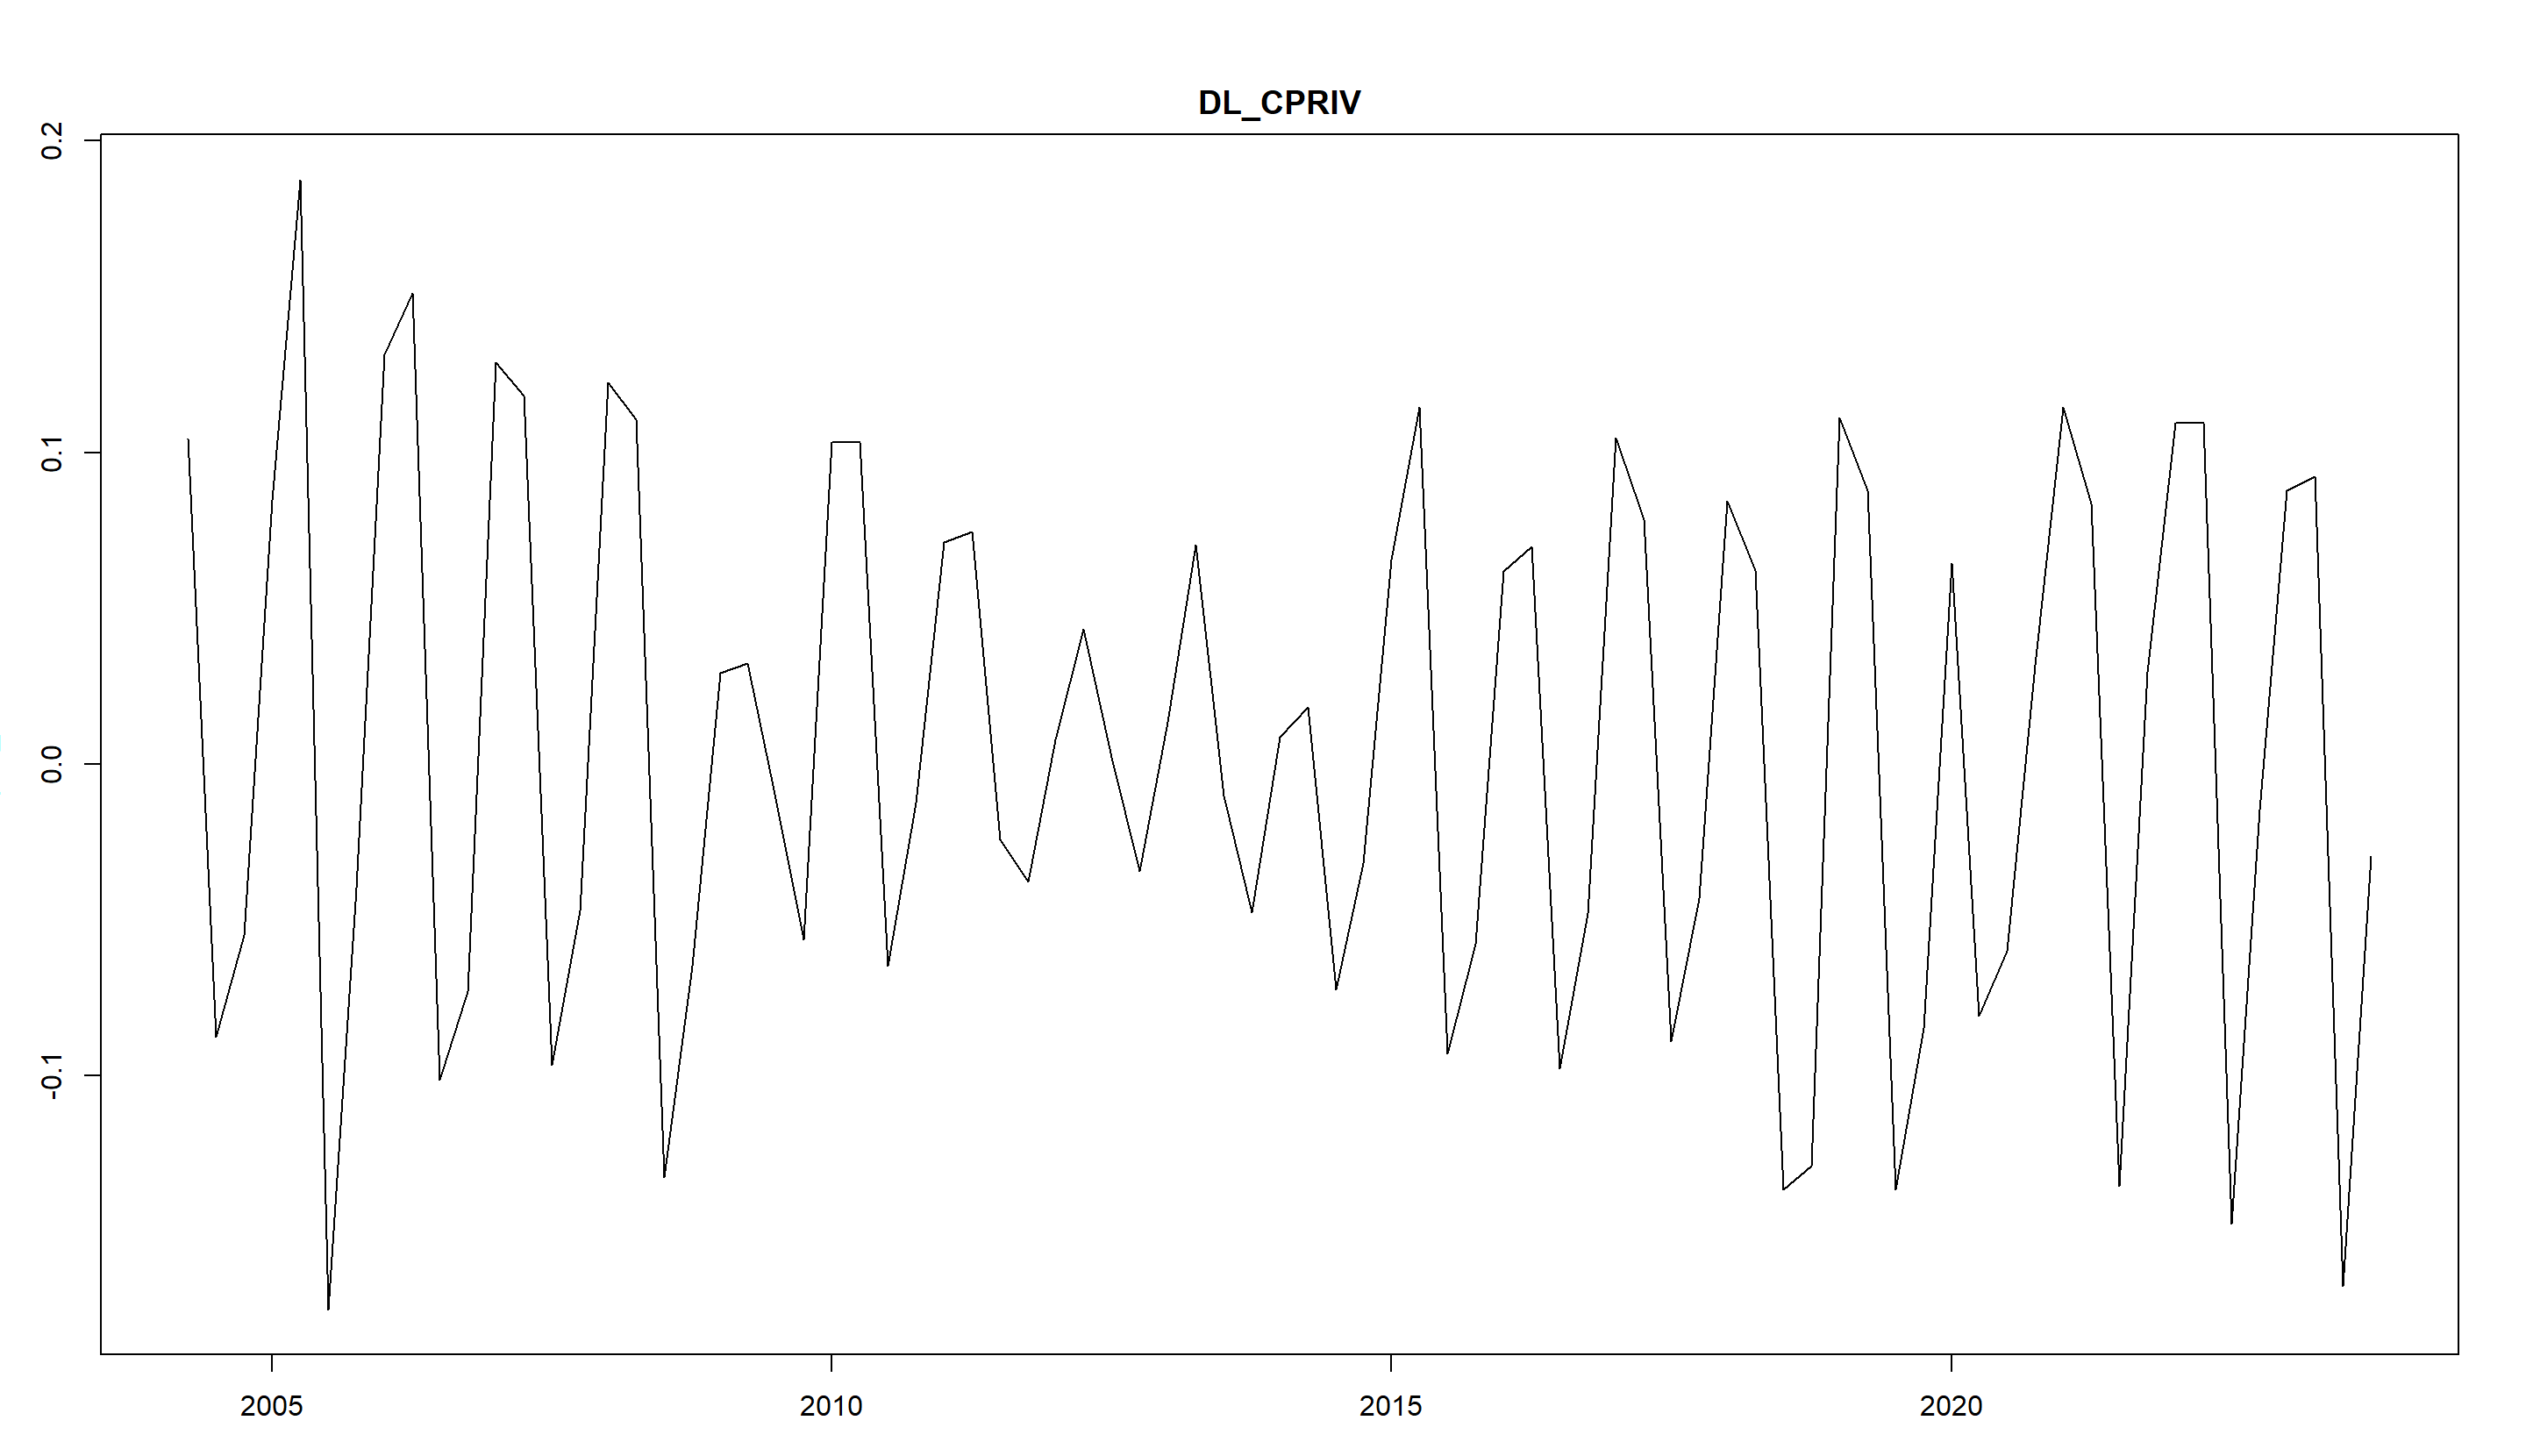
\includegraphics[width=0.8\textwidth]{1.png}
\caption{Evolución de la serie de consumo privado en diferencias logarítmicas (DL\_CPRIV).}
\label{fig:dl_cpriv}
\end{figure}

Las Figuras~\ref{fig:acf_cpriv} y~\ref{fig:pacf_cpriv} presentan, respectivamente, los correlogramas de autocorrelación simple y parcial de DL\_CPRIV. En la ACF se observan dependencias en los primeros rezagos y señales que pueden ser consistentes con una componente estacional trimestral, mientras que la PACF muestra una estructura más concentrada en pocos rezagos significativos. En conjunto, ambas evidencias sugieren que la dinámica del consumo privado puede representarse mediante especificaciones de bajo orden, aunque con espacio para incorporar términos estacionales si estos contribuyen a mejorar el desempeño predictivo del modelo.

\begin{figure}[H]
\centering
\begin{subfigure}[t]{0.48\textwidth}
\centering
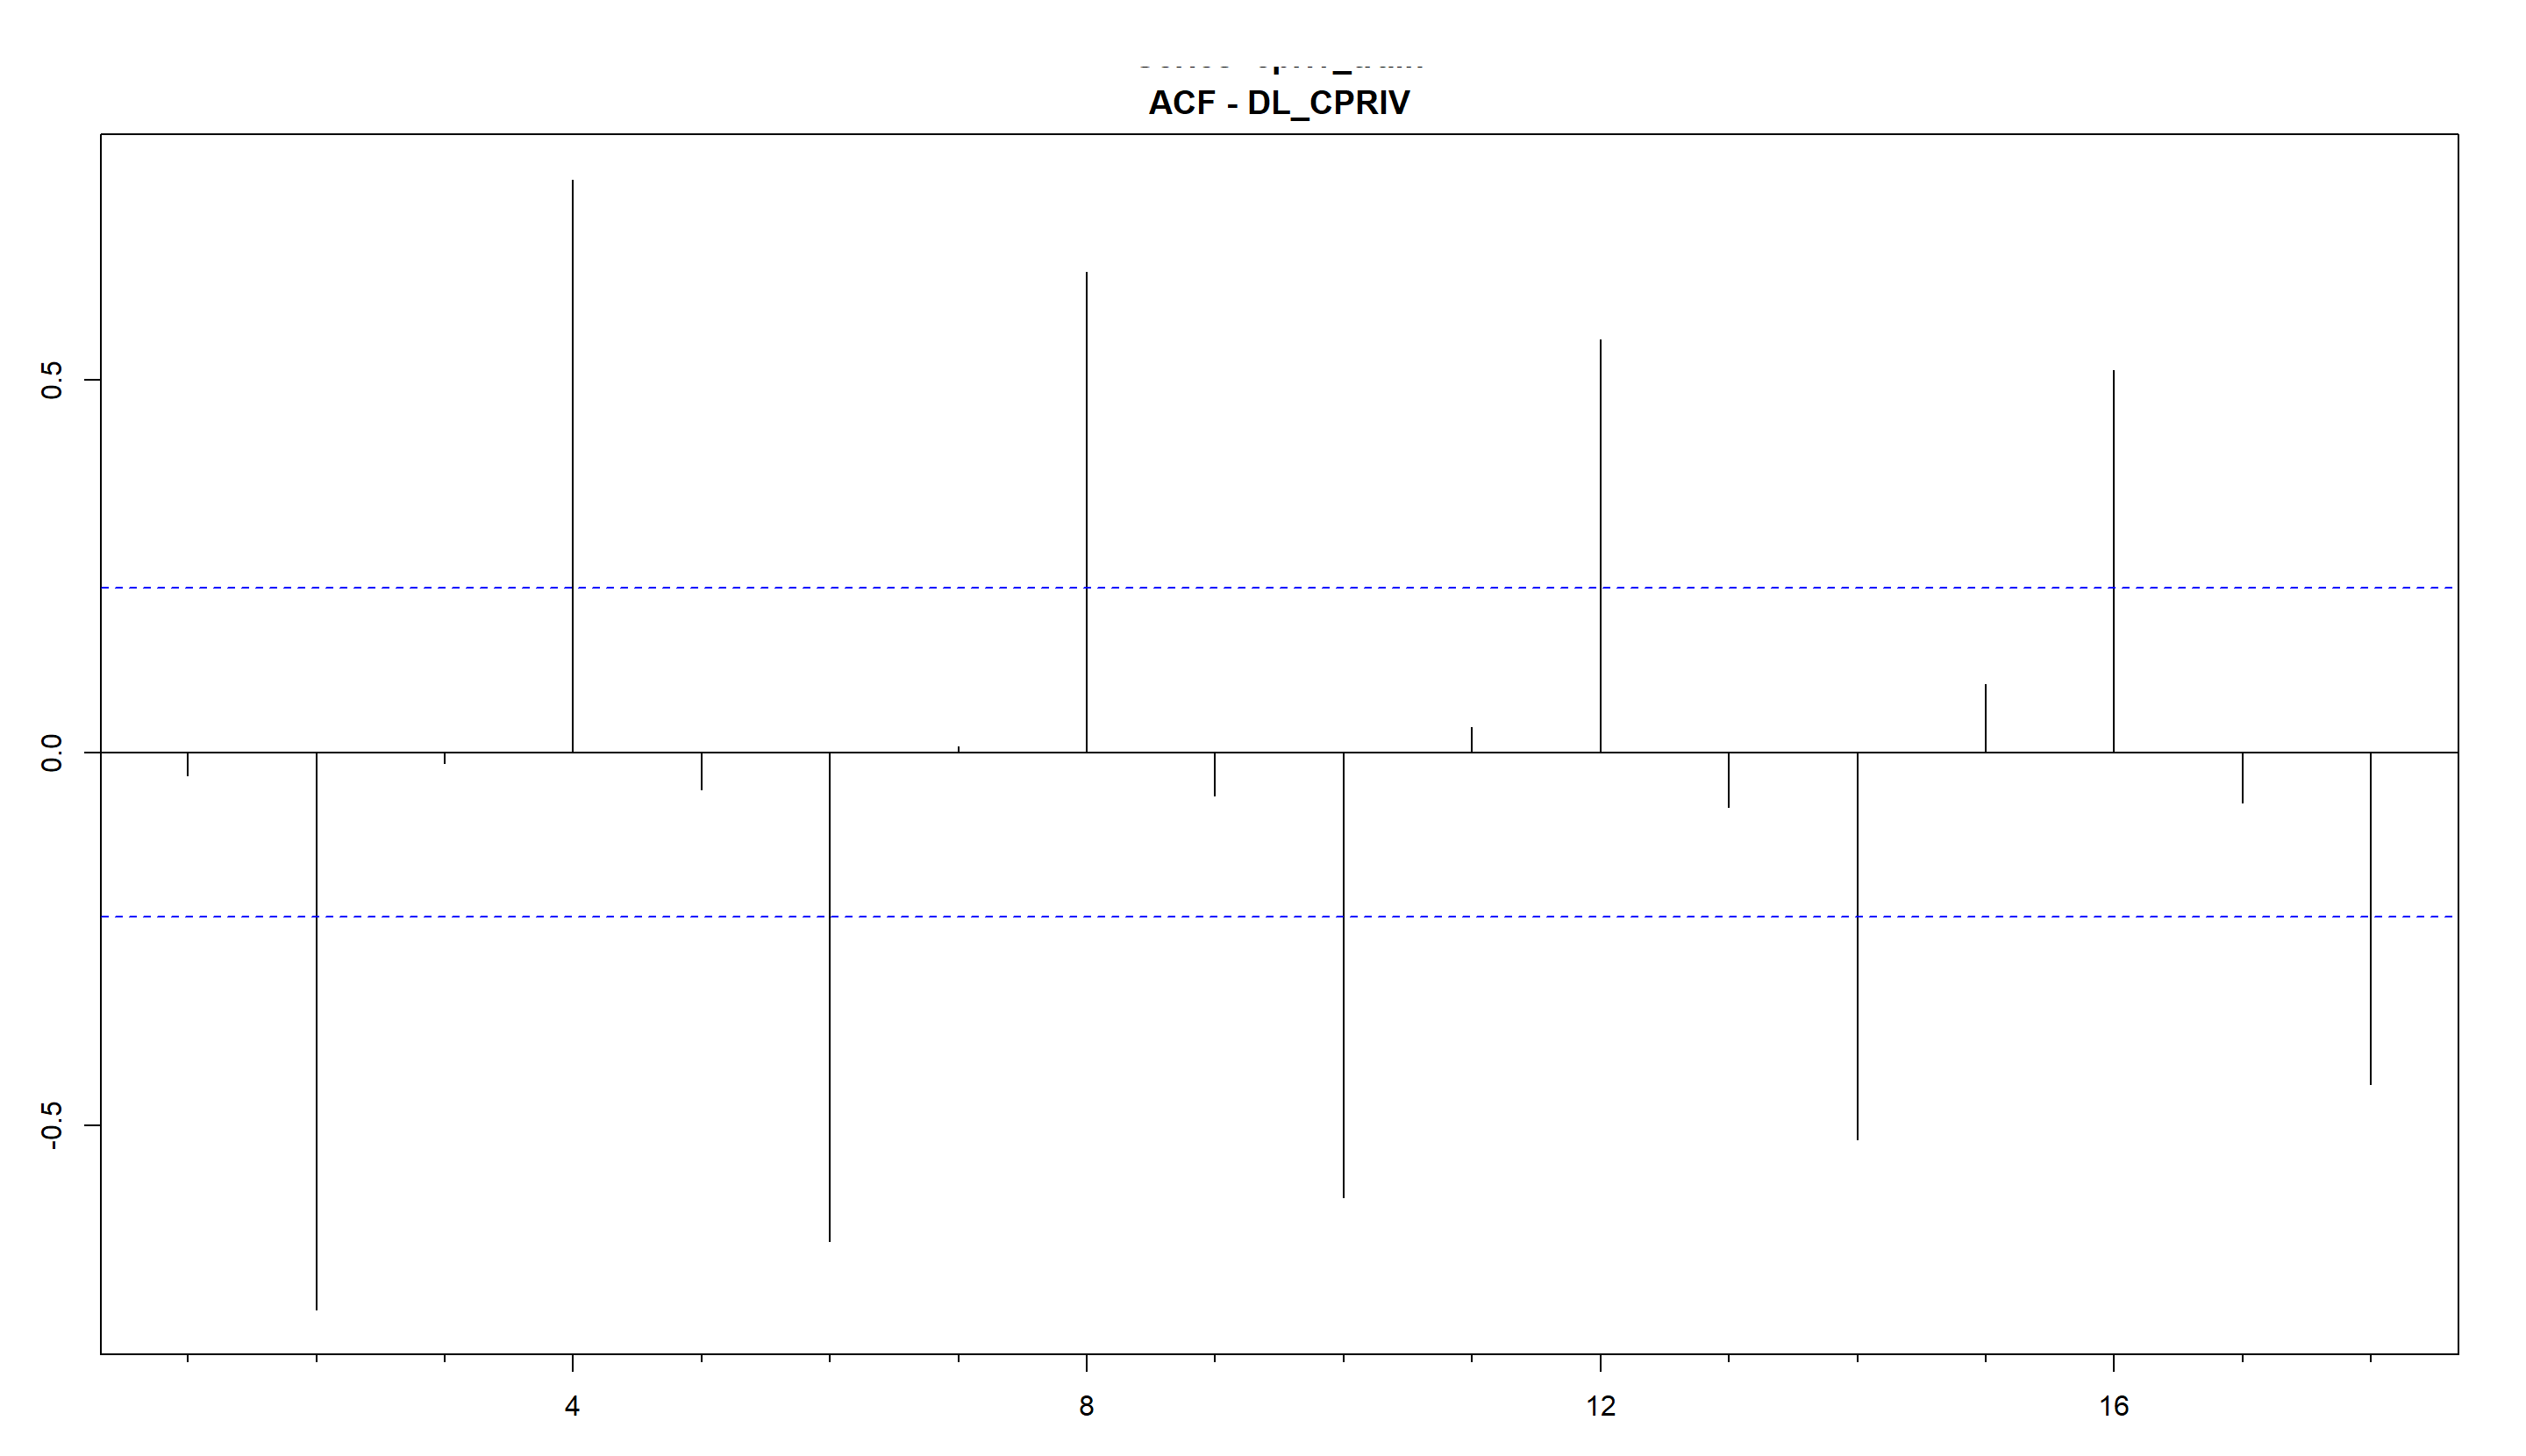
\includegraphics[width=\textwidth]{2.png}
\caption{Función de autocorrelación (ACF) de DL\_CPRIV.}
\label{fig:acf_cpriv}
\end{subfigure}
\hfill
\begin{subfigure}[t]{0.48\textwidth}
\centering
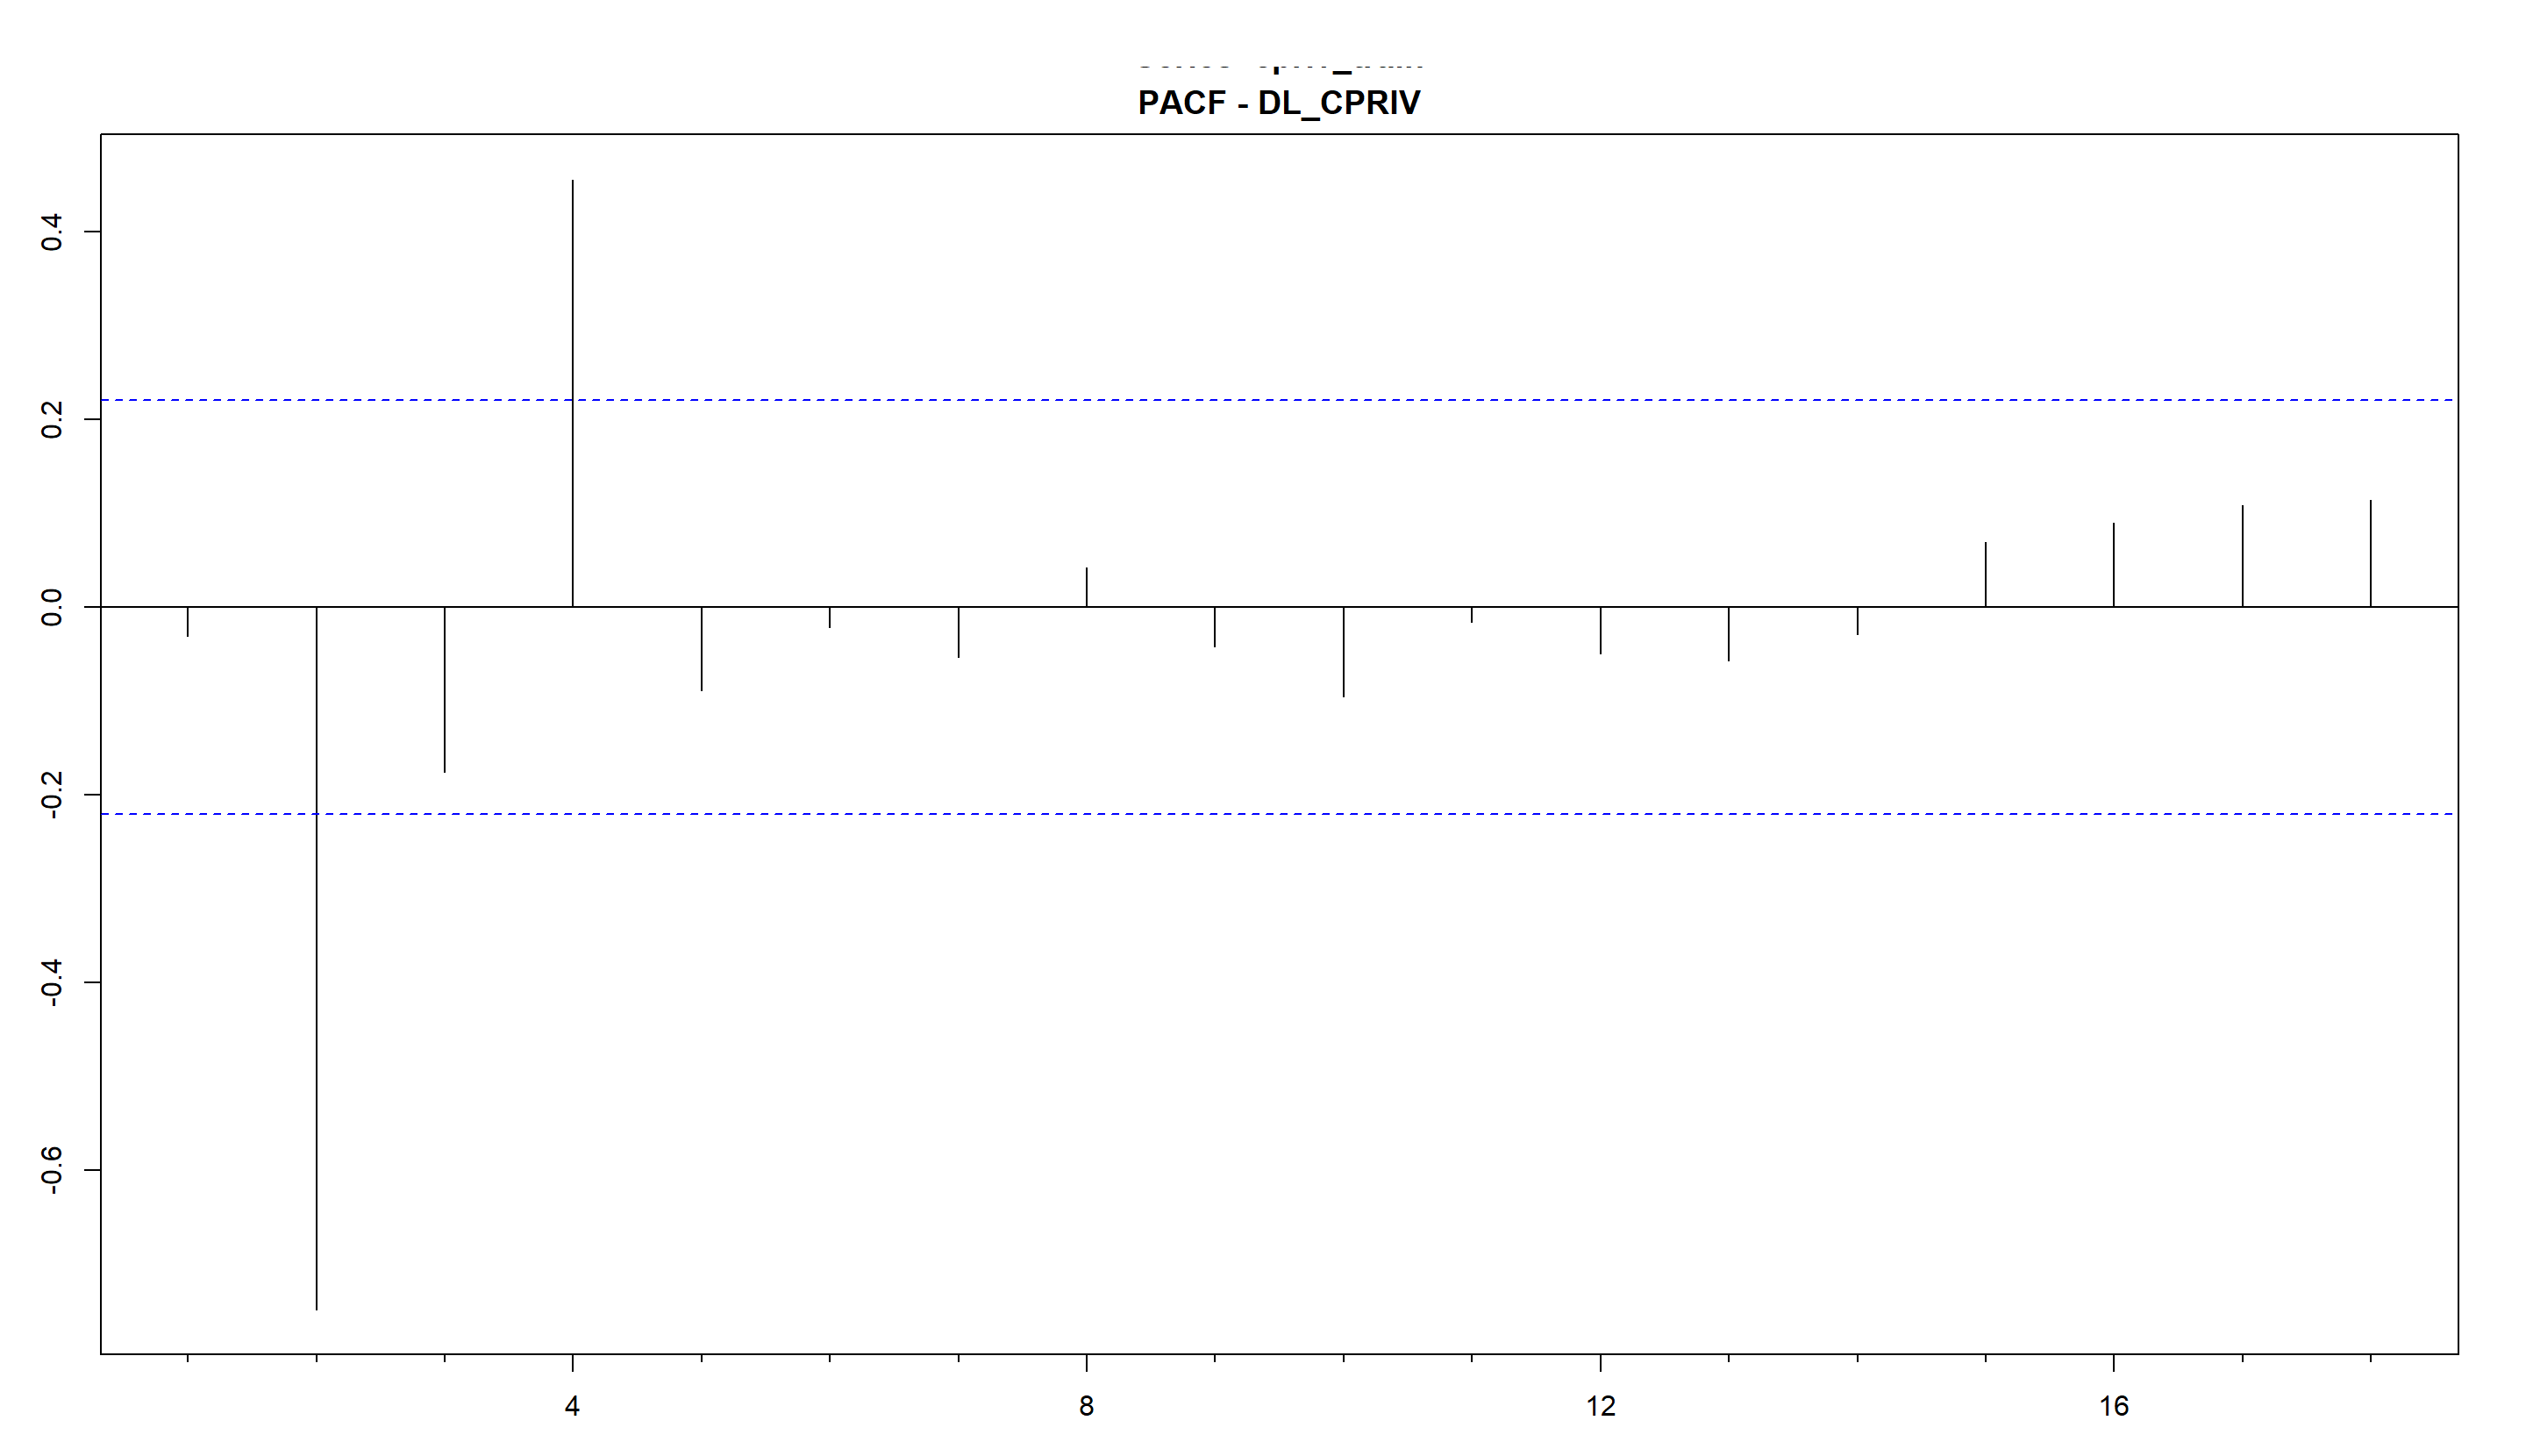
\includegraphics[width=\textwidth]{3.png}
\caption{Función de autocorrelación parcial (PACF) de DL\_CPRIV.}
\label{fig:pacf_cpriv}
\end{subfigure}
\end{figure}

El Cuadro~\ref{tab:sarima_cpriv} resume la comparación entre las especificaciones SARIMA candidatas estimadas sobre la serie original de DL\_CPRIV. Los resultados muestran un desempeño dentro de la muestra muy similar entre los tres modelos considerados, aunque la especificación automática presenta el menor AIC, lo que sugiere una leve ventaja en términos de ajuste relativo y parsimonia. En conjunto, la evidencia indica que la dinámica de la serie puede capturarse con modelos de baja complejidad y que las alternativas manuales no introducen mejoras sustantivas respecto de la selección automática.

\begin{table}[H]
\centering
\caption{Comparación de modelos SARIMA – DL\_CPRIV}
\label{tab:sarima_cpriv}
\begin{tabular}{lcccccc}
\hline
Modelo & AIC & RMSE & MAE & MAPE & MASE & ACF (res.) \\
\hline
SARIMA automático & -242.61 & 0.045064 & 0.033145 & 116.63 & 0.8420 & 0.0075 \\
SARIMA MA(1)      & -240.61 & 0.045064 & 0.033143 & 116.65 & 0.8419 & 0.0063 \\
SARIMA AR(1)      & -240.61 & 0.045064 & 0.033144 & 116.64 & 0.8420 & 0.0067 \\
\hline
\end{tabular}
\end{table}

El Cuadro~\ref{tab:diag_cpriv} presenta los diagnósticos residuales de los modelos estimados. Los p-valores del test de Ljung-Box y del estadístico Box-Ljung son elevados en todos los casos, lo que indica que no queda evidencia relevante de autocorrelación serial en los residuos. Por lo tanto, las tres especificaciones resultan estadísticamente admisibles desde el punto de vista del diagnóstico, aunque nuevamente el modelo automático conserva una ligera ventaja al combinar buen ajuste con una especificación parsimoniosa.

\begin{table}[H]
\centering
\caption{Diagnóstico de residuos – DL\_CPRIV}
\label{tab:diag_cpriv}
\begin{tabular}{lcc}
\hline
Modelo & Ljung-Box (p-valor) & Box-Ljung (p-valor) \\
\hline
SARIMA automático & 0.8602 & 0.9515 \\
SARIMA MA(1)      & 0.7768 & 0.9520 \\
SARIMA AR(1)      & 0.7765 & 0.9518 \\
\hline
\end{tabular}
\end{table}

Finalmente, el Cuadro~\ref{tab:forecast_cpriv} reporta la evaluación fuera de muestra para el período 2024--2025. Las métricas de RMSE, MAE, MAPE y U de Theil son prácticamente idénticas entre los tres modelos a la precisión reportada, lo que sugiere que la elección entre estas especificaciones no altera de manera significativa la capacidad predictiva. En ese contexto, el modelo SARIMA automático aparece como una opción razonable para continuar el análisis, dado que ofrece un desempeño comparable al de las alternativas manuales sin requerir una estructura más compleja.

\begin{table}[H]
\centering
\caption{Evaluación de desempeño predictivo (fuera de muestra) – DL\_CPRIV}
\label{tab:forecast_cpriv}
\begin{tabular}{lcccc}
\hline
Modelo & RMSE & MAE & MAPE & U de Theil \\
\hline
SARIMA automático & 0.03514 & 0.02986 & 73.48 & 0.2015 \\
SARIMA MA(1)      & 0.03514 & 0.02986 & 73.48 & 0.2015 \\
SARIMA AR(1)      & 0.03514 & 0.02986 & 73.48 & 0.2015 \\
\hline
\end{tabular}
\end{table}

La Figura~\ref{fig:dl_cpriv_sa} presenta la serie de consumo privado una vez removido el componente estacional mediante el procedimiento X-13. En comparación con la serie original, la trayectoria desestacionalizada conserva las fluctuaciones de corto plazo alrededor de cero, pero exhibe una dinámica más depurada del patrón periódico, lo que facilita concentrar el análisis en la persistencia no estacional y en la identificación de modelos más parsimoniosos.

\begin{figure}[H]
\centering
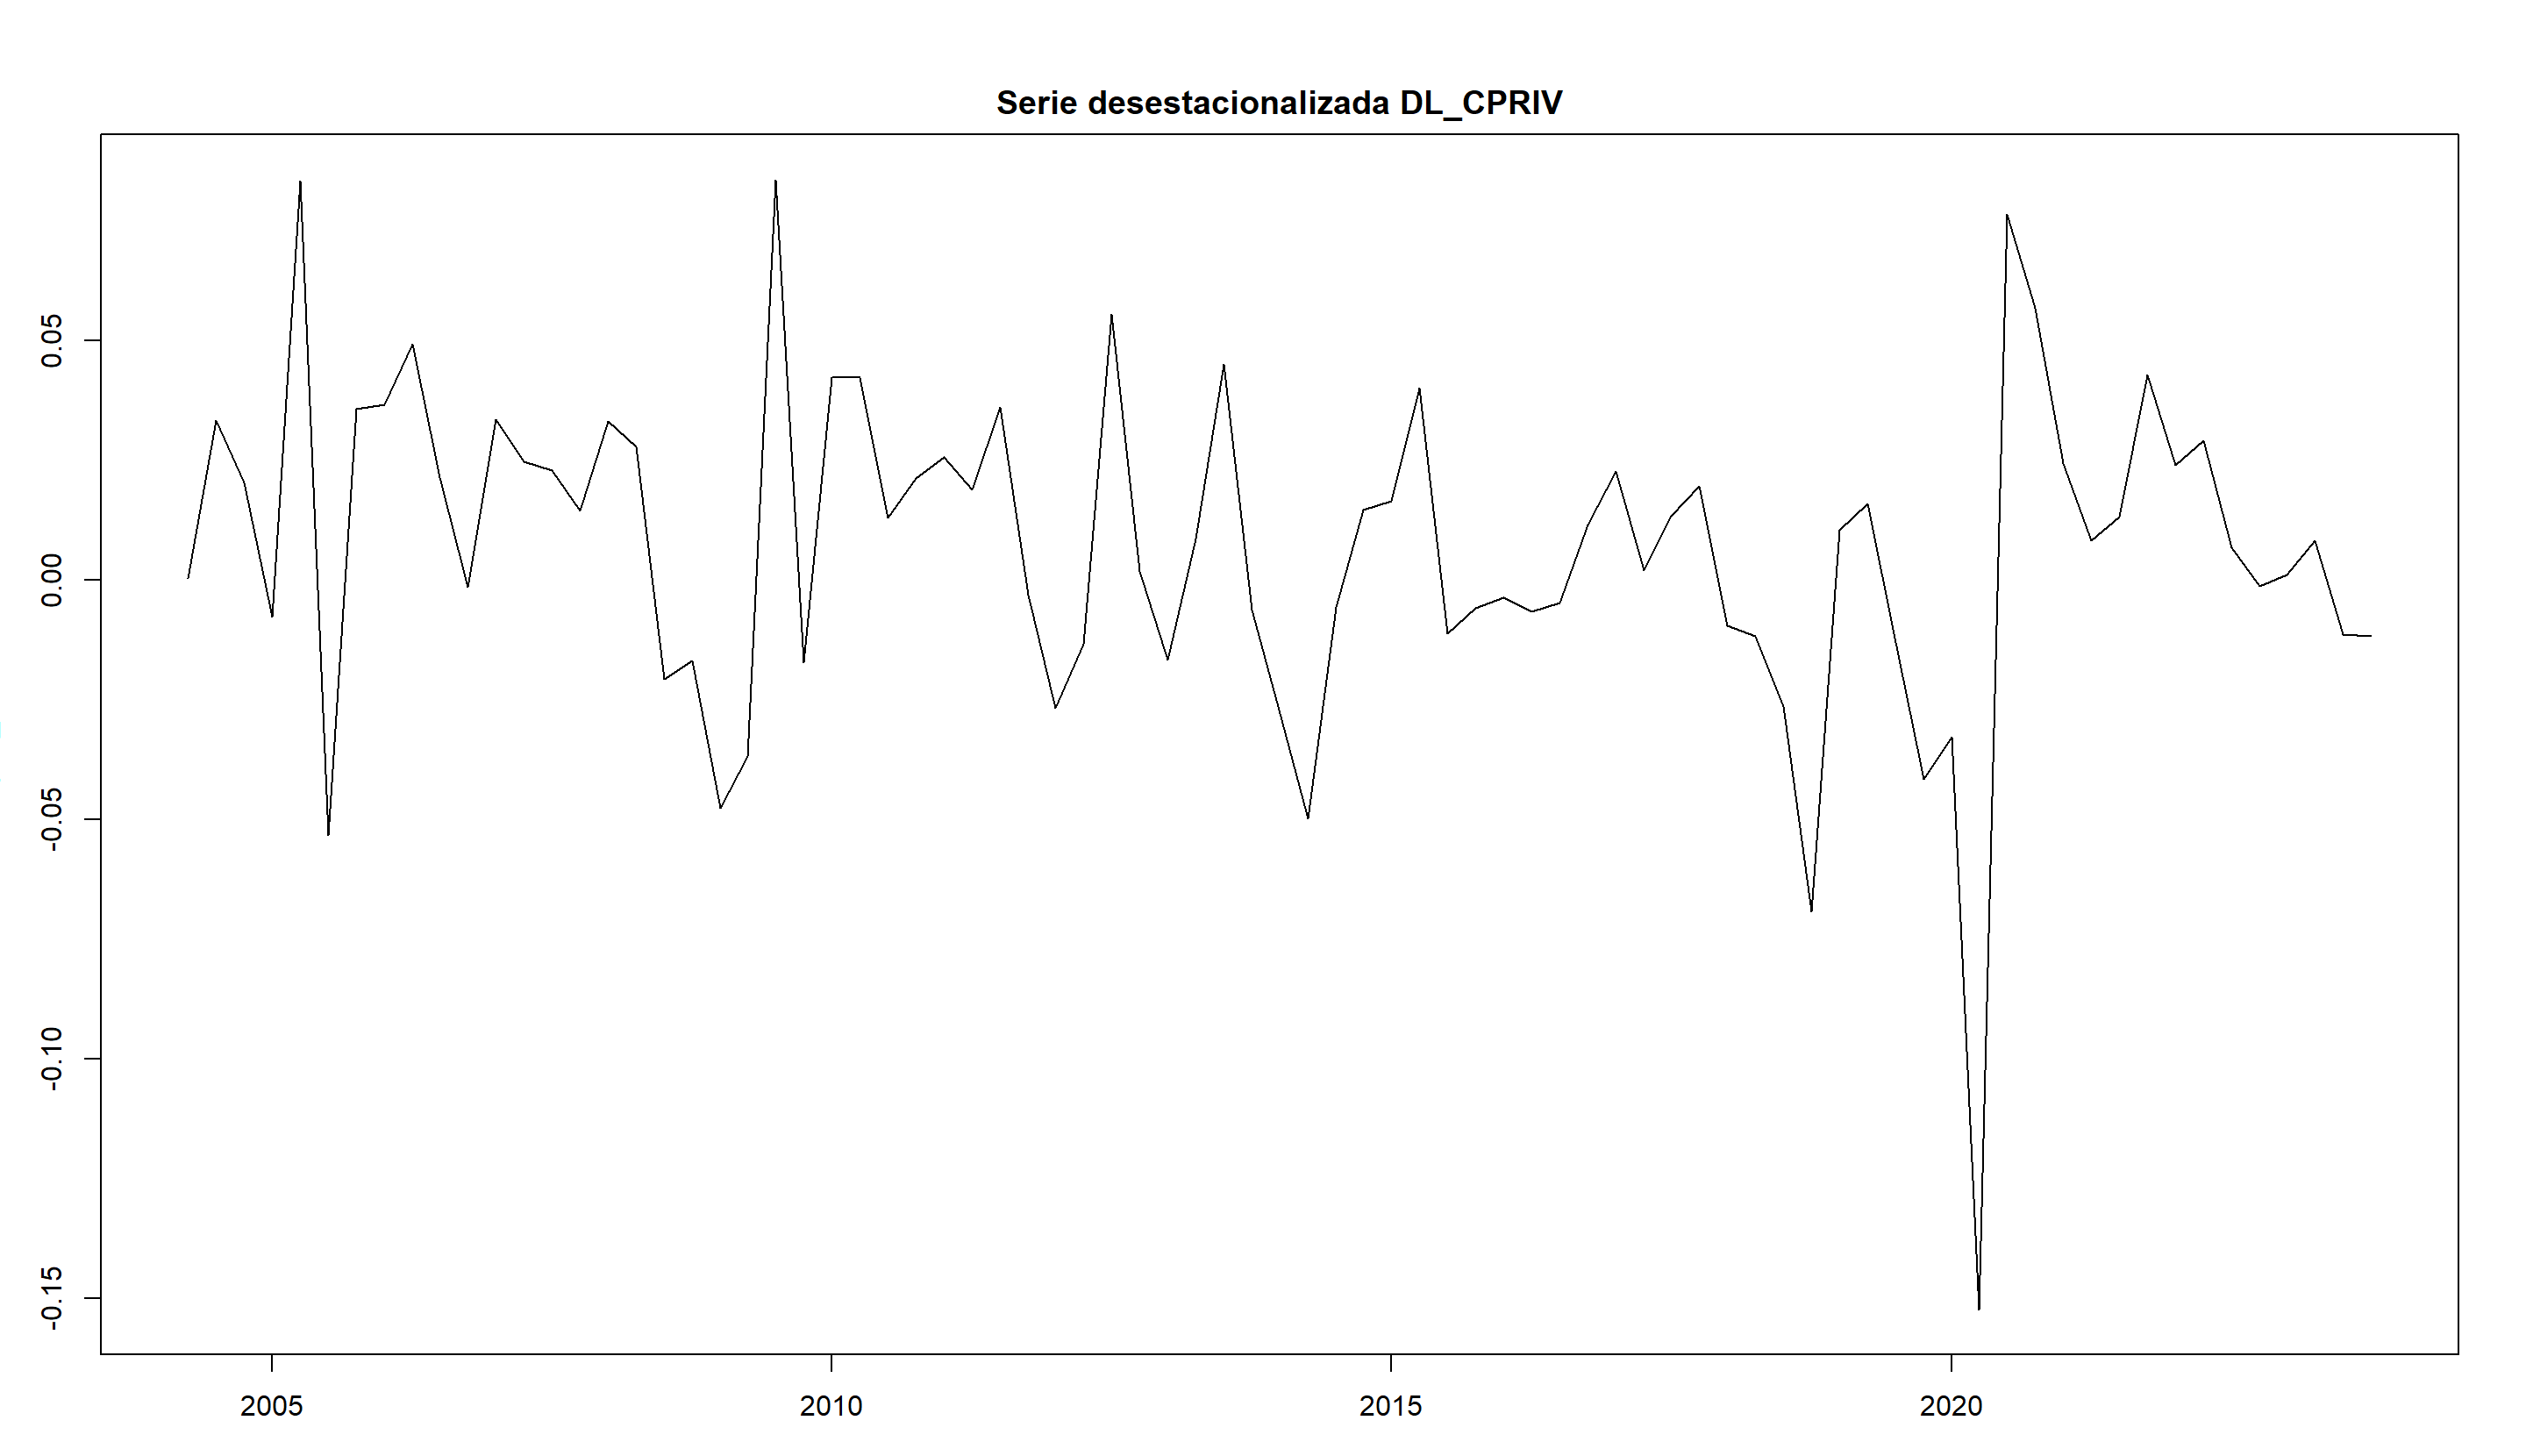
\includegraphics[width=0.8\textwidth]{4.png}
\caption{Serie de consumo privado en diferencias logarítmicas desestacionalizada (DL\_CPRIV), obtenida mediante el método X-13.}
\label{fig:dl_cpriv_sa}
\end{figure}

Las Figuras~\ref{fig:acf_cpriv_sa} y~\ref{fig:pacf_cpriv_sa} muestran los correlogramas de la serie desestacionalizada. La Figura~\ref{fig:acf_cpriv_sa} sugiere que, tras remover la estacionalidad, la dependencia serial se concentra en pocos rezagos y resulta menos marcada que en la serie original. A su vez, la Figura~\ref{fig:pacf_cpriv_sa} presenta una estructura acotada, compatible con la consideración de especificaciones ARMA de bajo orden para modelizar la dinámica remanente del consumo privado.

\begin{figure}[H]
\centering
\begin{subfigure}[t]{0.48\textwidth}
\centering
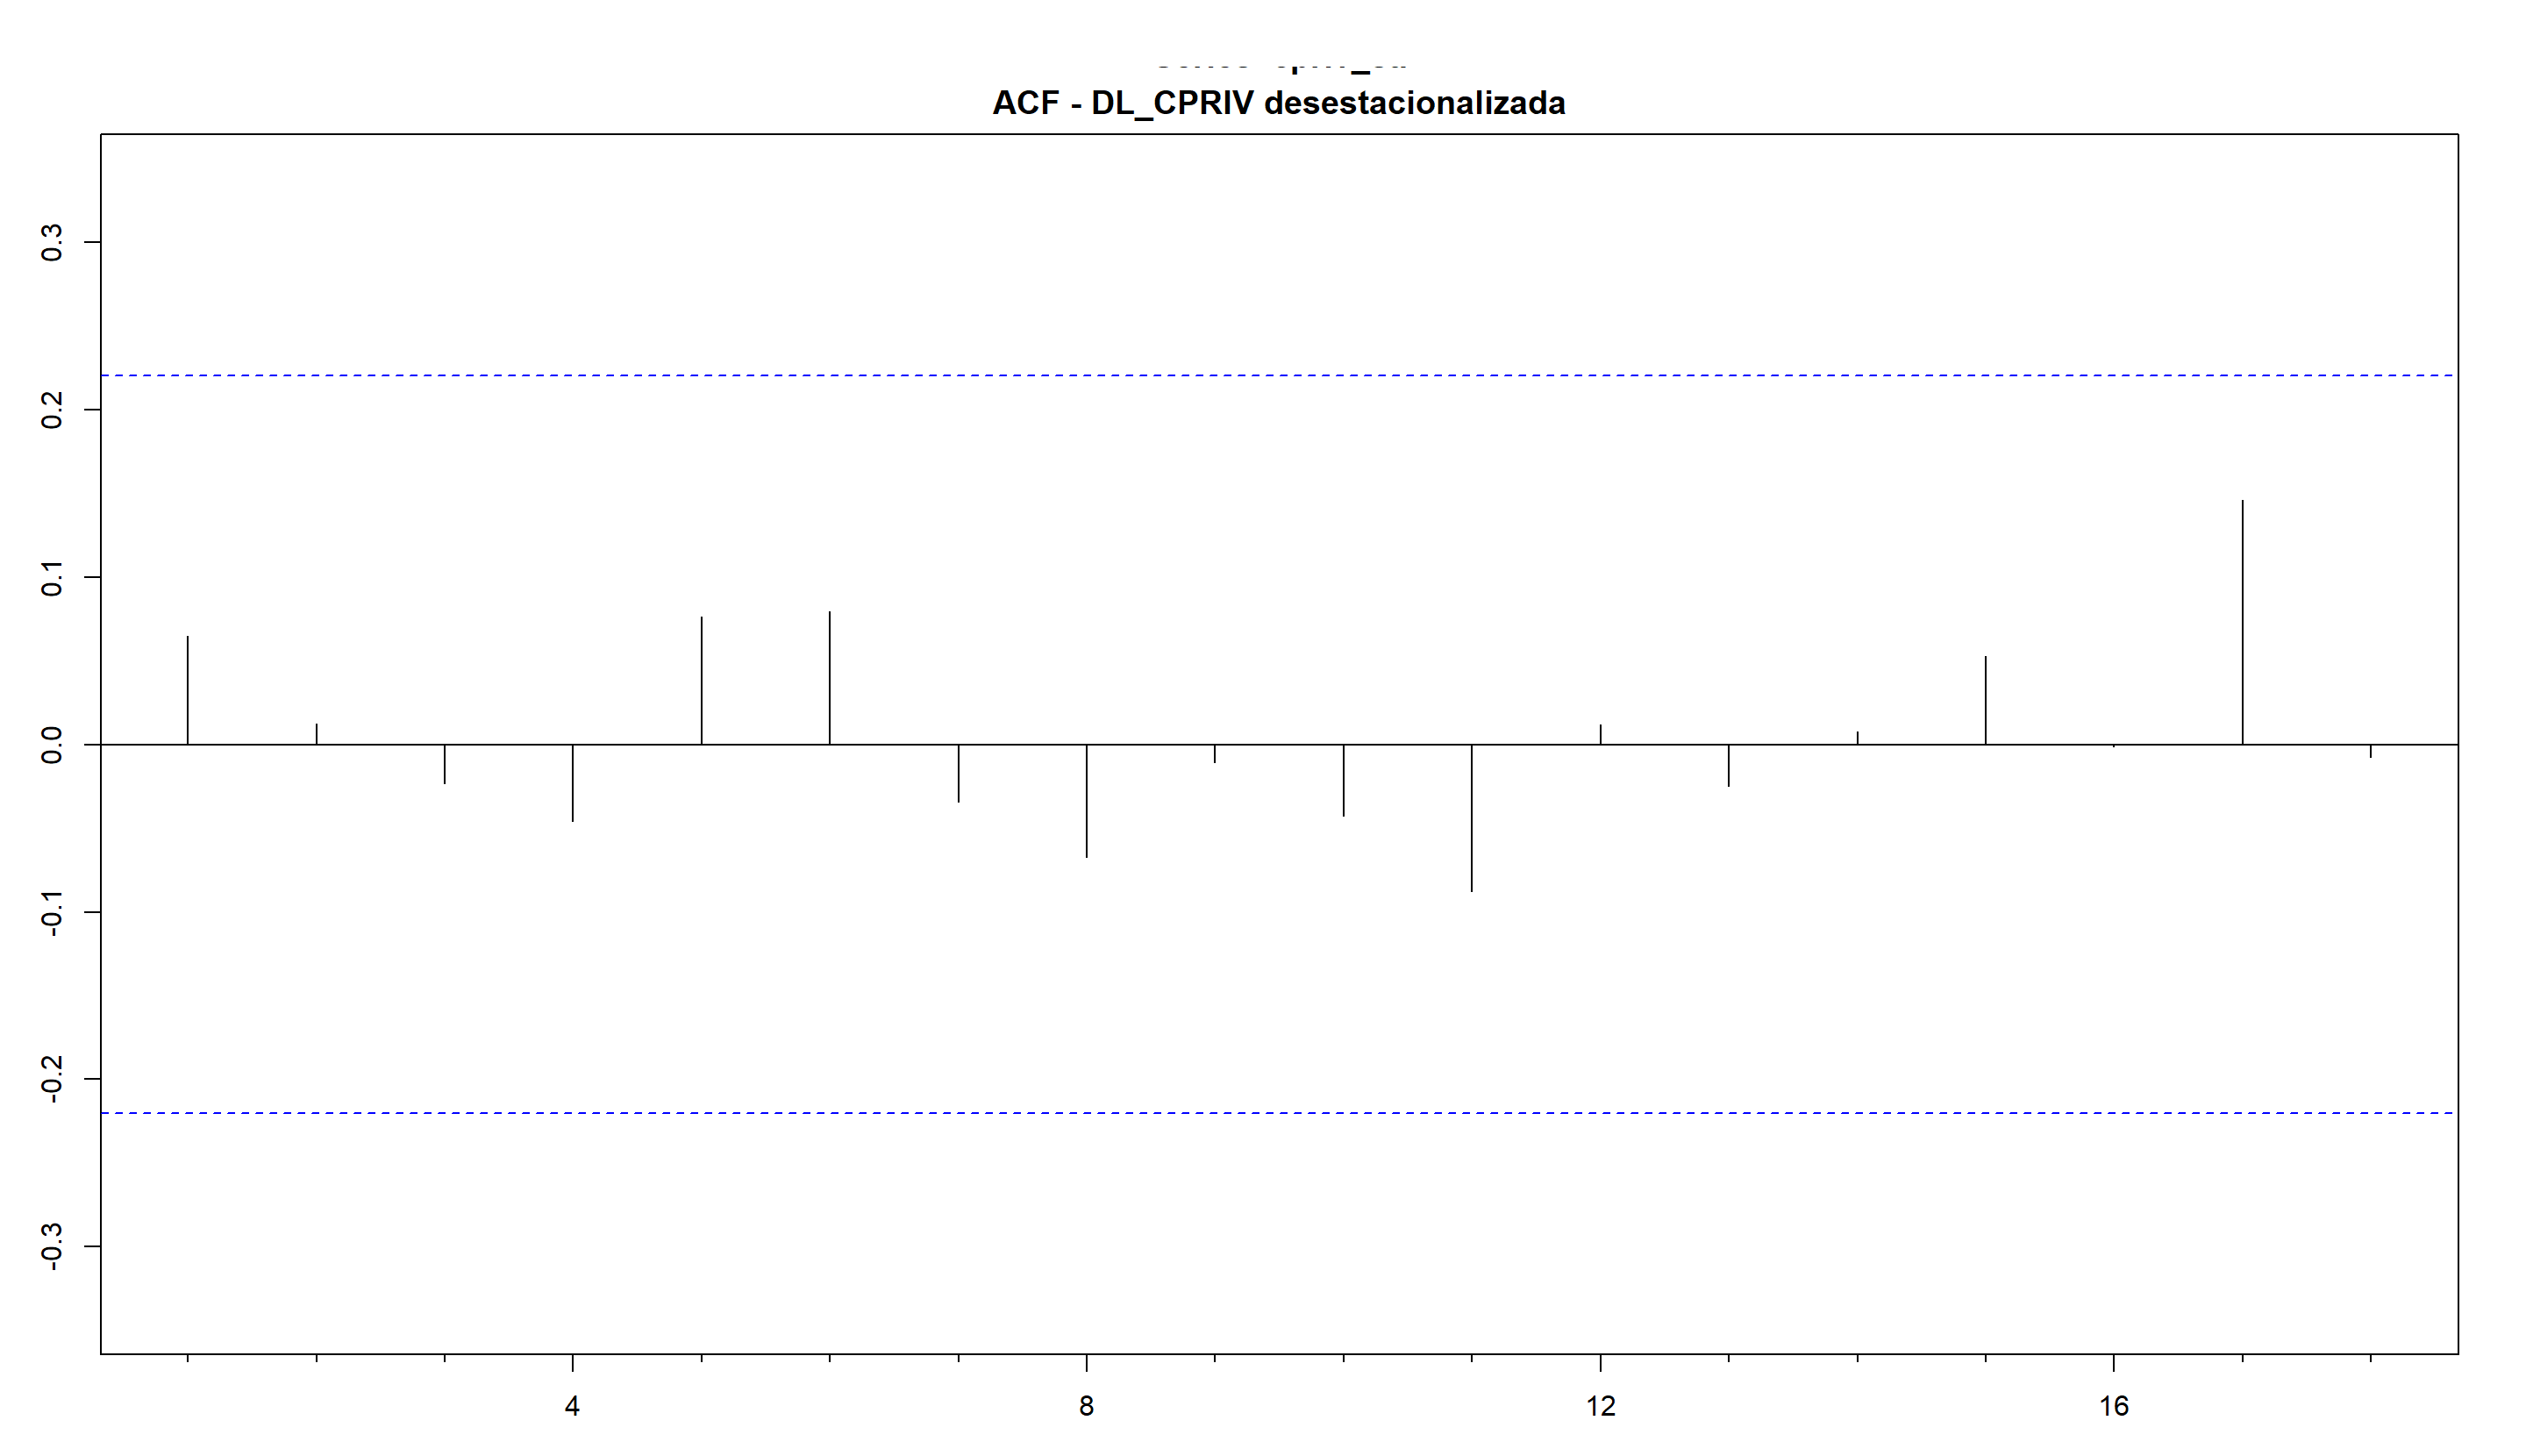
\includegraphics[width=\textwidth]{5.png}
\caption{Función de autocorrelación (ACF) de la serie desestacionalizada DL\_CPRIV.}
\label{fig:acf_cpriv_sa}
\end{subfigure}
\hfill
\begin{subfigure}[t]{0.48\textwidth}
\centering
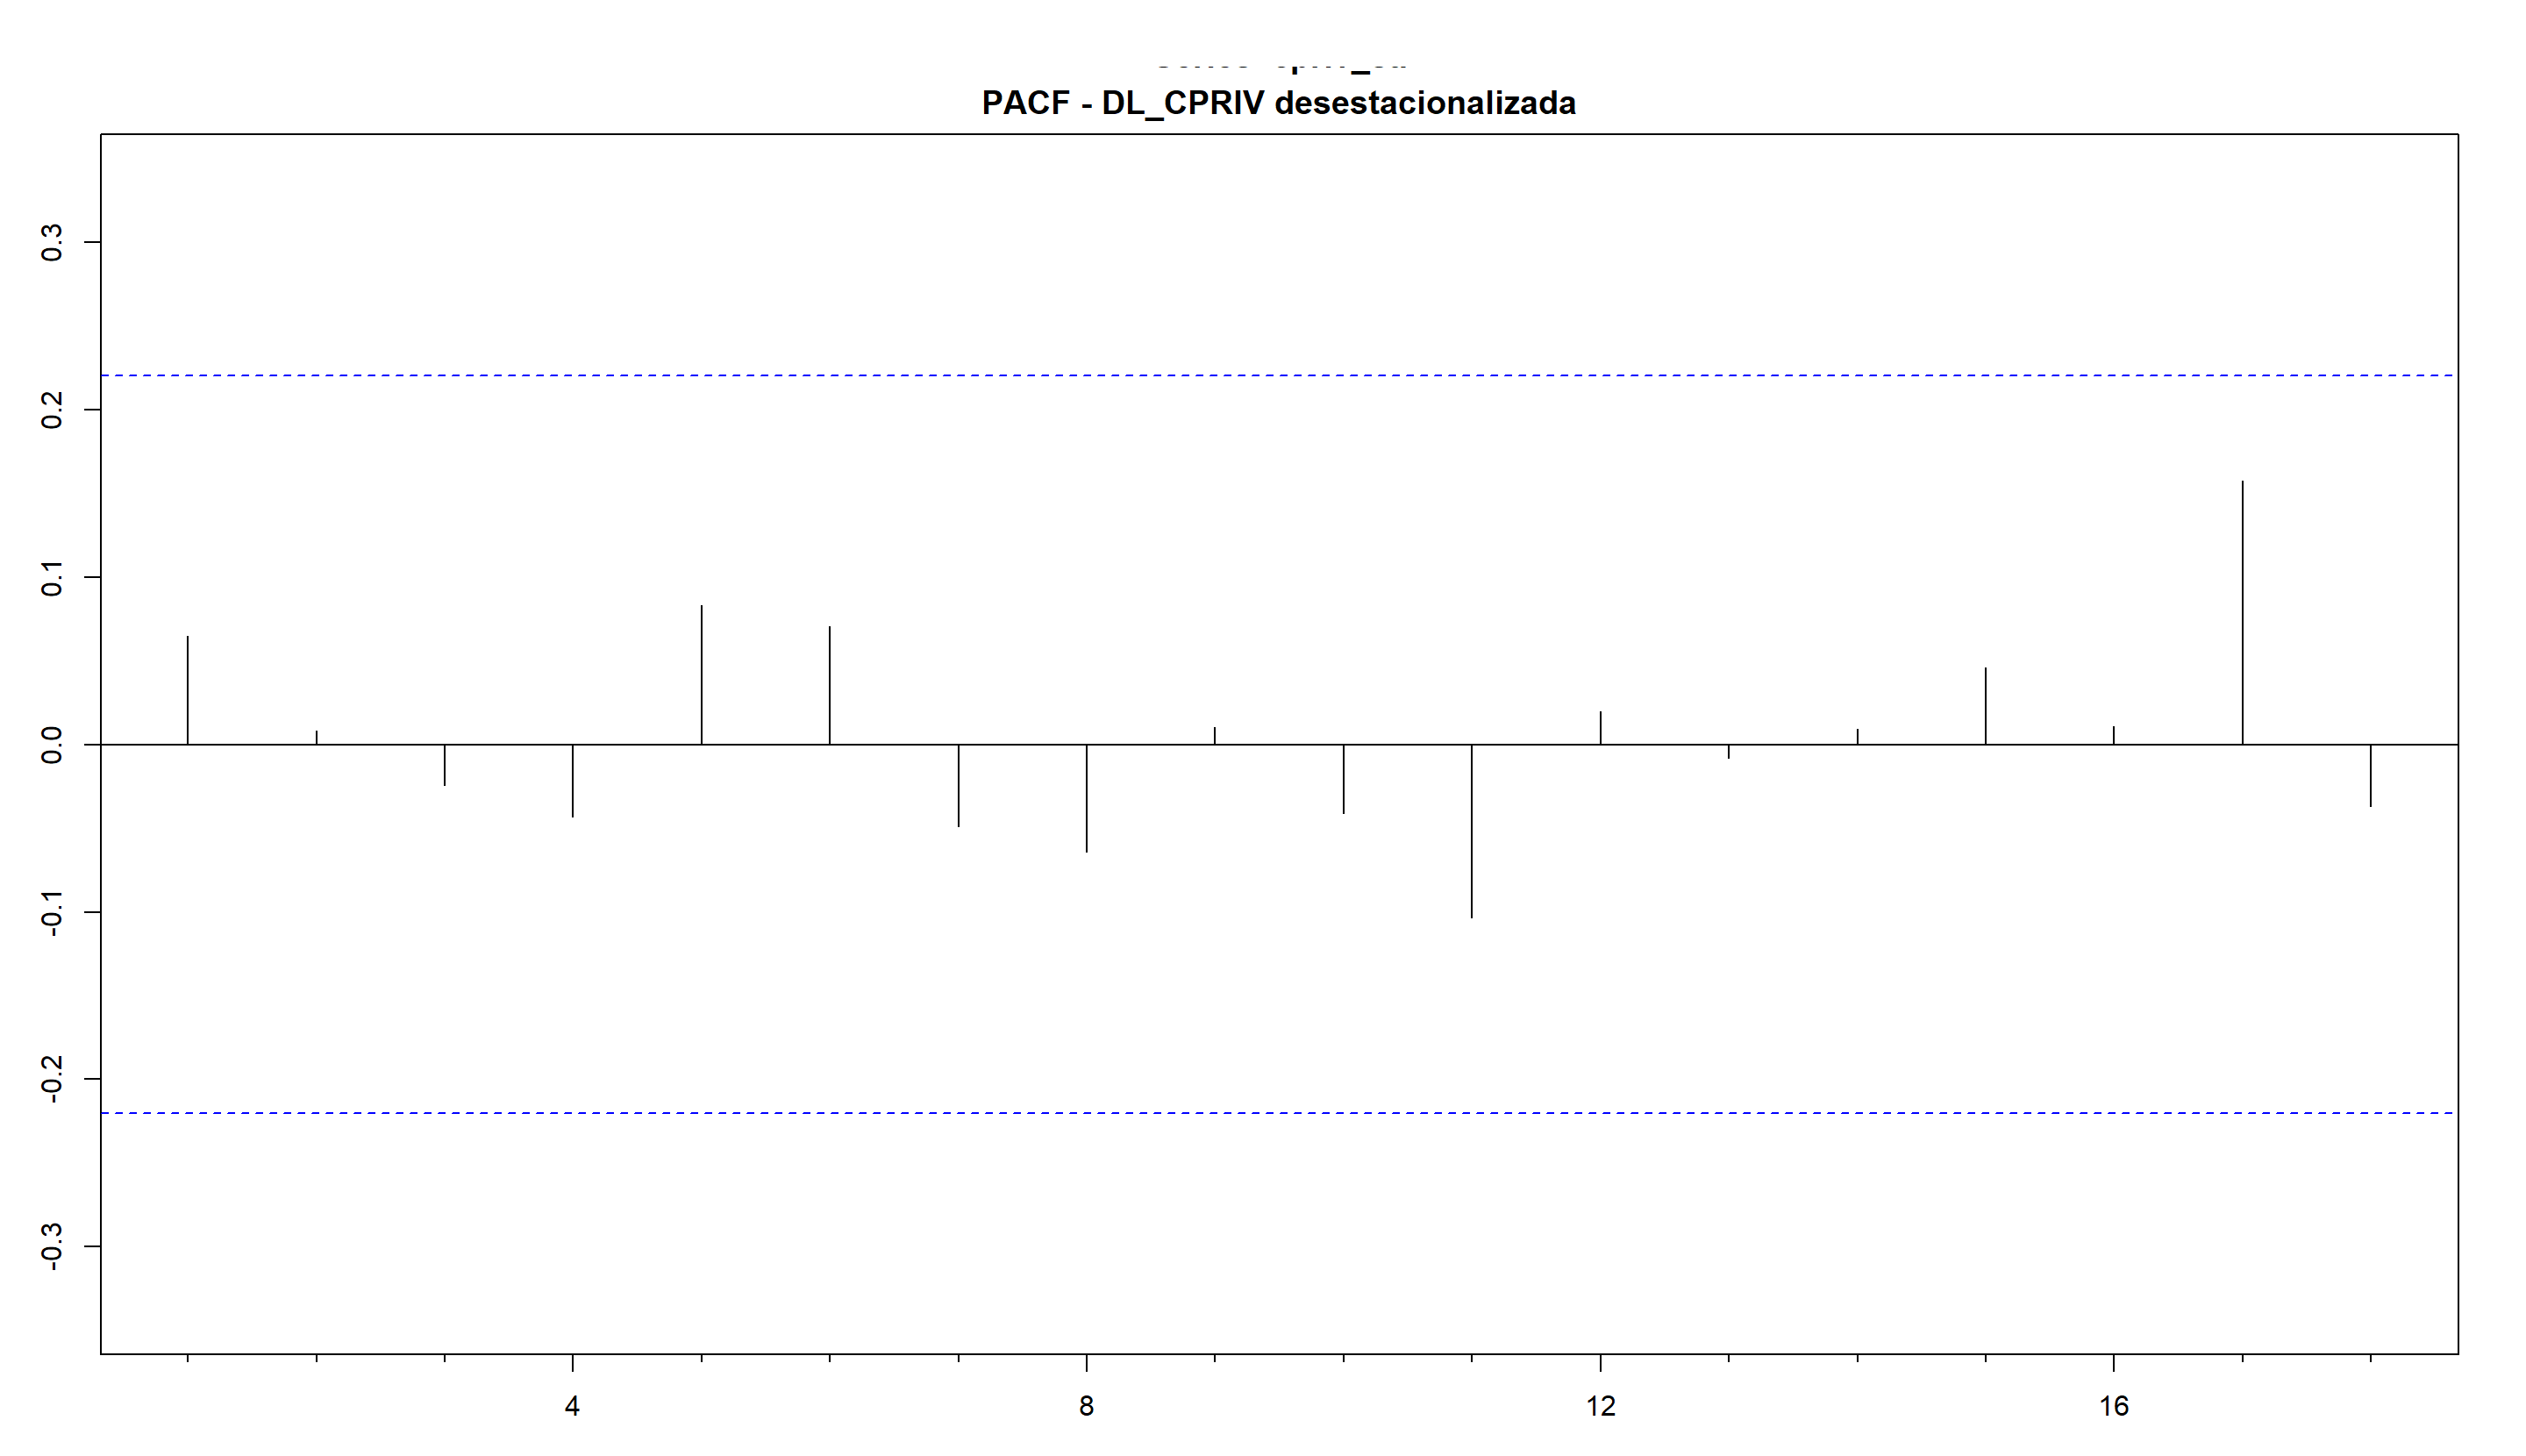
\includegraphics[width=\textwidth]{6.png}
\caption{Función de autocorrelación parcial (PACF) de la serie desestacionalizada DL\_CPRIV.}
\label{fig:pacf_cpriv_sa}
\end{subfigure}
\end{figure}

El Cuadro~\ref{tab:arma_sa_cpriv} resume la comparación entre los modelos estimados sobre la serie desestacionalizada de DL\_CPRIV. Un resultado relevante es que el modelo automático coincide con un proceso de ruido blanco con media, lo que sugiere que, una vez removida la estacionalidad, la persistencia remanente de la serie se reduce considerablemente. No obstante, la especificación ARMA(1,1) exhibe mejoras marginales en RMSE, MAE, MASE y autocorrelación residual, aunque a costa de un AIC menos favorable y de un MAPE algo más elevado. En consecuencia, el cuadro sugiere una disyuntiva entre parsimonia y pequeñas ganancias de ajuste, sin que emerja una diferencia concluyente entre ambas alternativas.

\begin{table}[H]
\centering
\caption{Comparación de modelos ARMA sobre serie desestacionalizada – DL\_CPRIV}
\label{tab:arma_sa_cpriv}
\begin{tabular}{lcccccc}
\hline
Modelo & AIC & RMSE & MAE & MAPE & MASE & ACF (res.) \\
\hline
ARMA automático (media) & -303.02 & 0.03466 & 0.02526 & 145.43 & 0.6700 & 0.06498 \\
ARMA(1,1)              & -299.35 & 0.03459 & 0.02509 & 147.83 & 0.6655 & 0.00048 \\
Ruido blanco (media)   & -303.02 & 0.03466 & 0.02526 & 145.43 & 0.6700 & 0.06498 \\
\hline
\end{tabular}
\end{table}

El Cuadro~\ref{tab:diag_sa_cpriv} presenta los diagnósticos residuales correspondientes a estas especificaciones. Los p-valores elevados en todos los casos indican que no queda evidencia de autocorrelación serial significativa en los residuos, por lo que los modelos considerados resultan adecuados desde el punto de vista estadístico. En particular, el ARMA(1,1) logra residuos prácticamente no autocorrelacionados y mantiene un diagnóstico satisfactorio, mientras que el modelo automático y el ruido blanco también superan ampliamente las pruebas de independencia. Así, el Cuadro~\ref{tab:diag_sa_cpriv} refuerza la idea de que, para la serie desestacionalizada, incluso modelos muy simples pueden ofrecer una representación aceptable de la dinámica observada.

\begin{table}[H]
\centering
\caption{Diagnóstico de residuos – serie desestacionalizada DL\_CPRIV}
\label{tab:diag_sa_cpriv}
\begin{tabular}{lcc}
\hline
Modelo & Ljung-Box (p-valor) & Box-Ljung (p-valor) \\
\hline
ARMA automático (media) & 0.9761 & 0.9951 \\
ARMA(1,1)              & 0.9394 & 0.9976 \\
Ruido blanco (media)   & 0.9761 & 0.9951 \\
\hline
\end{tabular}
\end{table}

El Cuadro~\ref{tab:forecast_sa_cpriv} reporta la evaluación fuera de muestra de los modelos estimados sobre la serie desestacionalizada de DL\_CPRIV. Los resultados muestran que la especificación ARMA(1,1) obtiene el mejor desempeño predictivo entre las alternativas consideradas, con valores ligeramente menores de RMSE, MAE, MAPE y U de Theil respecto del modelo automático y del ruido blanco con media, que vuelven a presentar resultados idénticos entre sí. Sin embargo, las diferencias son cuantitativamente reducidas, lo que sugiere que la desestacionalización deja una dinámica remanente relativamente débil y que las ganancias asociadas a una especificación algo más rica son solo marginales. Asimismo, la descomposición del U de Theil indica que la mayor parte del error proviene del componente de covarianza y no de sesgo o varianza, lo cual es consistente con pronósticos razonablemente centrados pero limitados para reproducir con precisión la variación puntual de la serie.

\begin{table}[H]
\centering
\caption{Evaluación de pronósticos – serie desestacionalizada DL\_CPRIV}
\label{tab:forecast_sa_cpriv}
\begin{tabular}{lccc}
\hline
Métrica & SA Auto & SA ARMA(1,1) & SA WN \\
\hline
RMSE         & 0.04021 & 0.04008 & 0.04021 \\
MAE          & 0.03533 & 0.03516 & 0.03533 \\
MAPE         & 91.65   & 91.31   & 91.65   \\
U de Theil   & 0.25516 & 0.25460 & 0.25516 \\
U sesgo      & 0.01210 & 0.01333 & 0.01210 \\
U varianza   & 0.00014 & 0.00006 & 0.00014 \\
U covarianza & 0.98775 & 0.98661 & 0.98775 \\
\hline
\end{tabular}
\end{table}

En conjunto, el Cuadro~\ref{tab:global_cpriv} sintetiza la comparación entre las estrategias de modelización para DL\_CPRIV. La evidencia es clara en favor de los modelos estimados sobre la serie original: las tres especificaciones SARIMA superan de manera sistemática a las alternativas basadas en la serie desestacionalizada en RMSE, MAE, MAPE y U de Theil. Aunque dentro del enfoque desestacionalizado el ARMA(1,1) ofrece una mejora marginal respecto de las otras variantes, esa ganancia no alcanza para revertir la superioridad de la modelización directa de la estacionalidad. Adicionalmente, la descomposición del U de Theil sugiere que los modelos sobre la serie ajustada concentran casi todo su error en el componente de covarianza, mientras que las especificaciones SARIMA distribuyen en menor medida ese error y logran un mejor desempeño global. Por lo tanto, para la serie de consumo privado, los resultados indican que conservar e incorporar explícitamente la estacionalidad dentro del modelo produce pronósticos más precisos que removerla ex ante.

\begin{table}[H]
\centering
\caption{Comparación global de métodos de pronóstico – DL\_CPRIV}
\label{tab:global_cpriv}
\resizebox{\textwidth}{!}{
\begin{tabular}{lcccccc}
\hline
Métrica & SARIMA Auto & SARIMA MA & SARIMA AR & SA Auto & SA ARMA(1,1) & SA WN \\
\hline
RMSE         & 0.03514 & 0.03514 & 0.03514 & 0.04021 & 0.04008 & 0.04021 \\
MAE          & 0.02986 & 0.02986 & 0.02986 & 0.03533 & 0.03516 & 0.03533 \\
MAPE         & 73.48   & 73.48   & 73.48   & 91.65   & 91.31   & 91.65   \\
U de Theil   & 0.20148 & 0.20147 & 0.20147 & 0.25516 & 0.25460 & 0.25516 \\
U sesgo      & 0.05075 & 0.05083 & 0.05080 & 0.01210 & 0.01333 & 0.01210 \\
U varianza   & 0.24949 & 0.24950 & 0.24949 & 0.00014 & 0.00006 & 0.00014 \\
U covarianza & 0.69976 & 0.69968 & 0.69970 & 0.98775 & 0.98661 & 0.98775 \\
\hline
\end{tabular}
}
\end{table}

El análisis del consumo privado mostró que, para esa serie, la modelización directa de la estacionalidad mediante especificaciones SARIMA ofrece un mejor desempeño predictivo que la estrategia basada en desestacionalización previa. A continuación, se replica el mismo esquema de evaluación para la serie de exportaciones, con el objetivo de examinar si esa conclusión se mantiene en una variable con una dinámica potencialmente más volátil y con rasgos estacionales diferentes. De este modo, la comparación entre ambas estrategias vuelve a organizarse en torno al análisis gráfico inicial, la identificación mediante correlogramas, la estimación de modelos candidatos, el diagnóstico residual y la evaluación de pronósticos fuera de muestra.

\subsection{Exportaciones (DL\_EXPO)}

La Figura~\ref{fig:dl_expo} presenta la evolución de la serie DL\_EXPO en diferencias logarítmicas. En línea con su interpretación como aproximación a la tasa de crecimiento trimestral de las exportaciones, la serie fluctúa alrededor de cero y no exhibe una tendencia persistente en media. Sin embargo, muestra una volatilidad relativamente elevada, con oscilaciones frecuentes entre valores positivos y negativos y con episodios puntuales de movimientos más intensos ---como el fuerte aumento observado alrededor de 2010 y la caída marcada en torno a 2020---, lo que sugiere que la dinámica de las exportaciones se encuentra expuesta a shocks transitorios y a cambios abruptos en el entorno macroeconómico.

\begin{figure}[H]
\centering
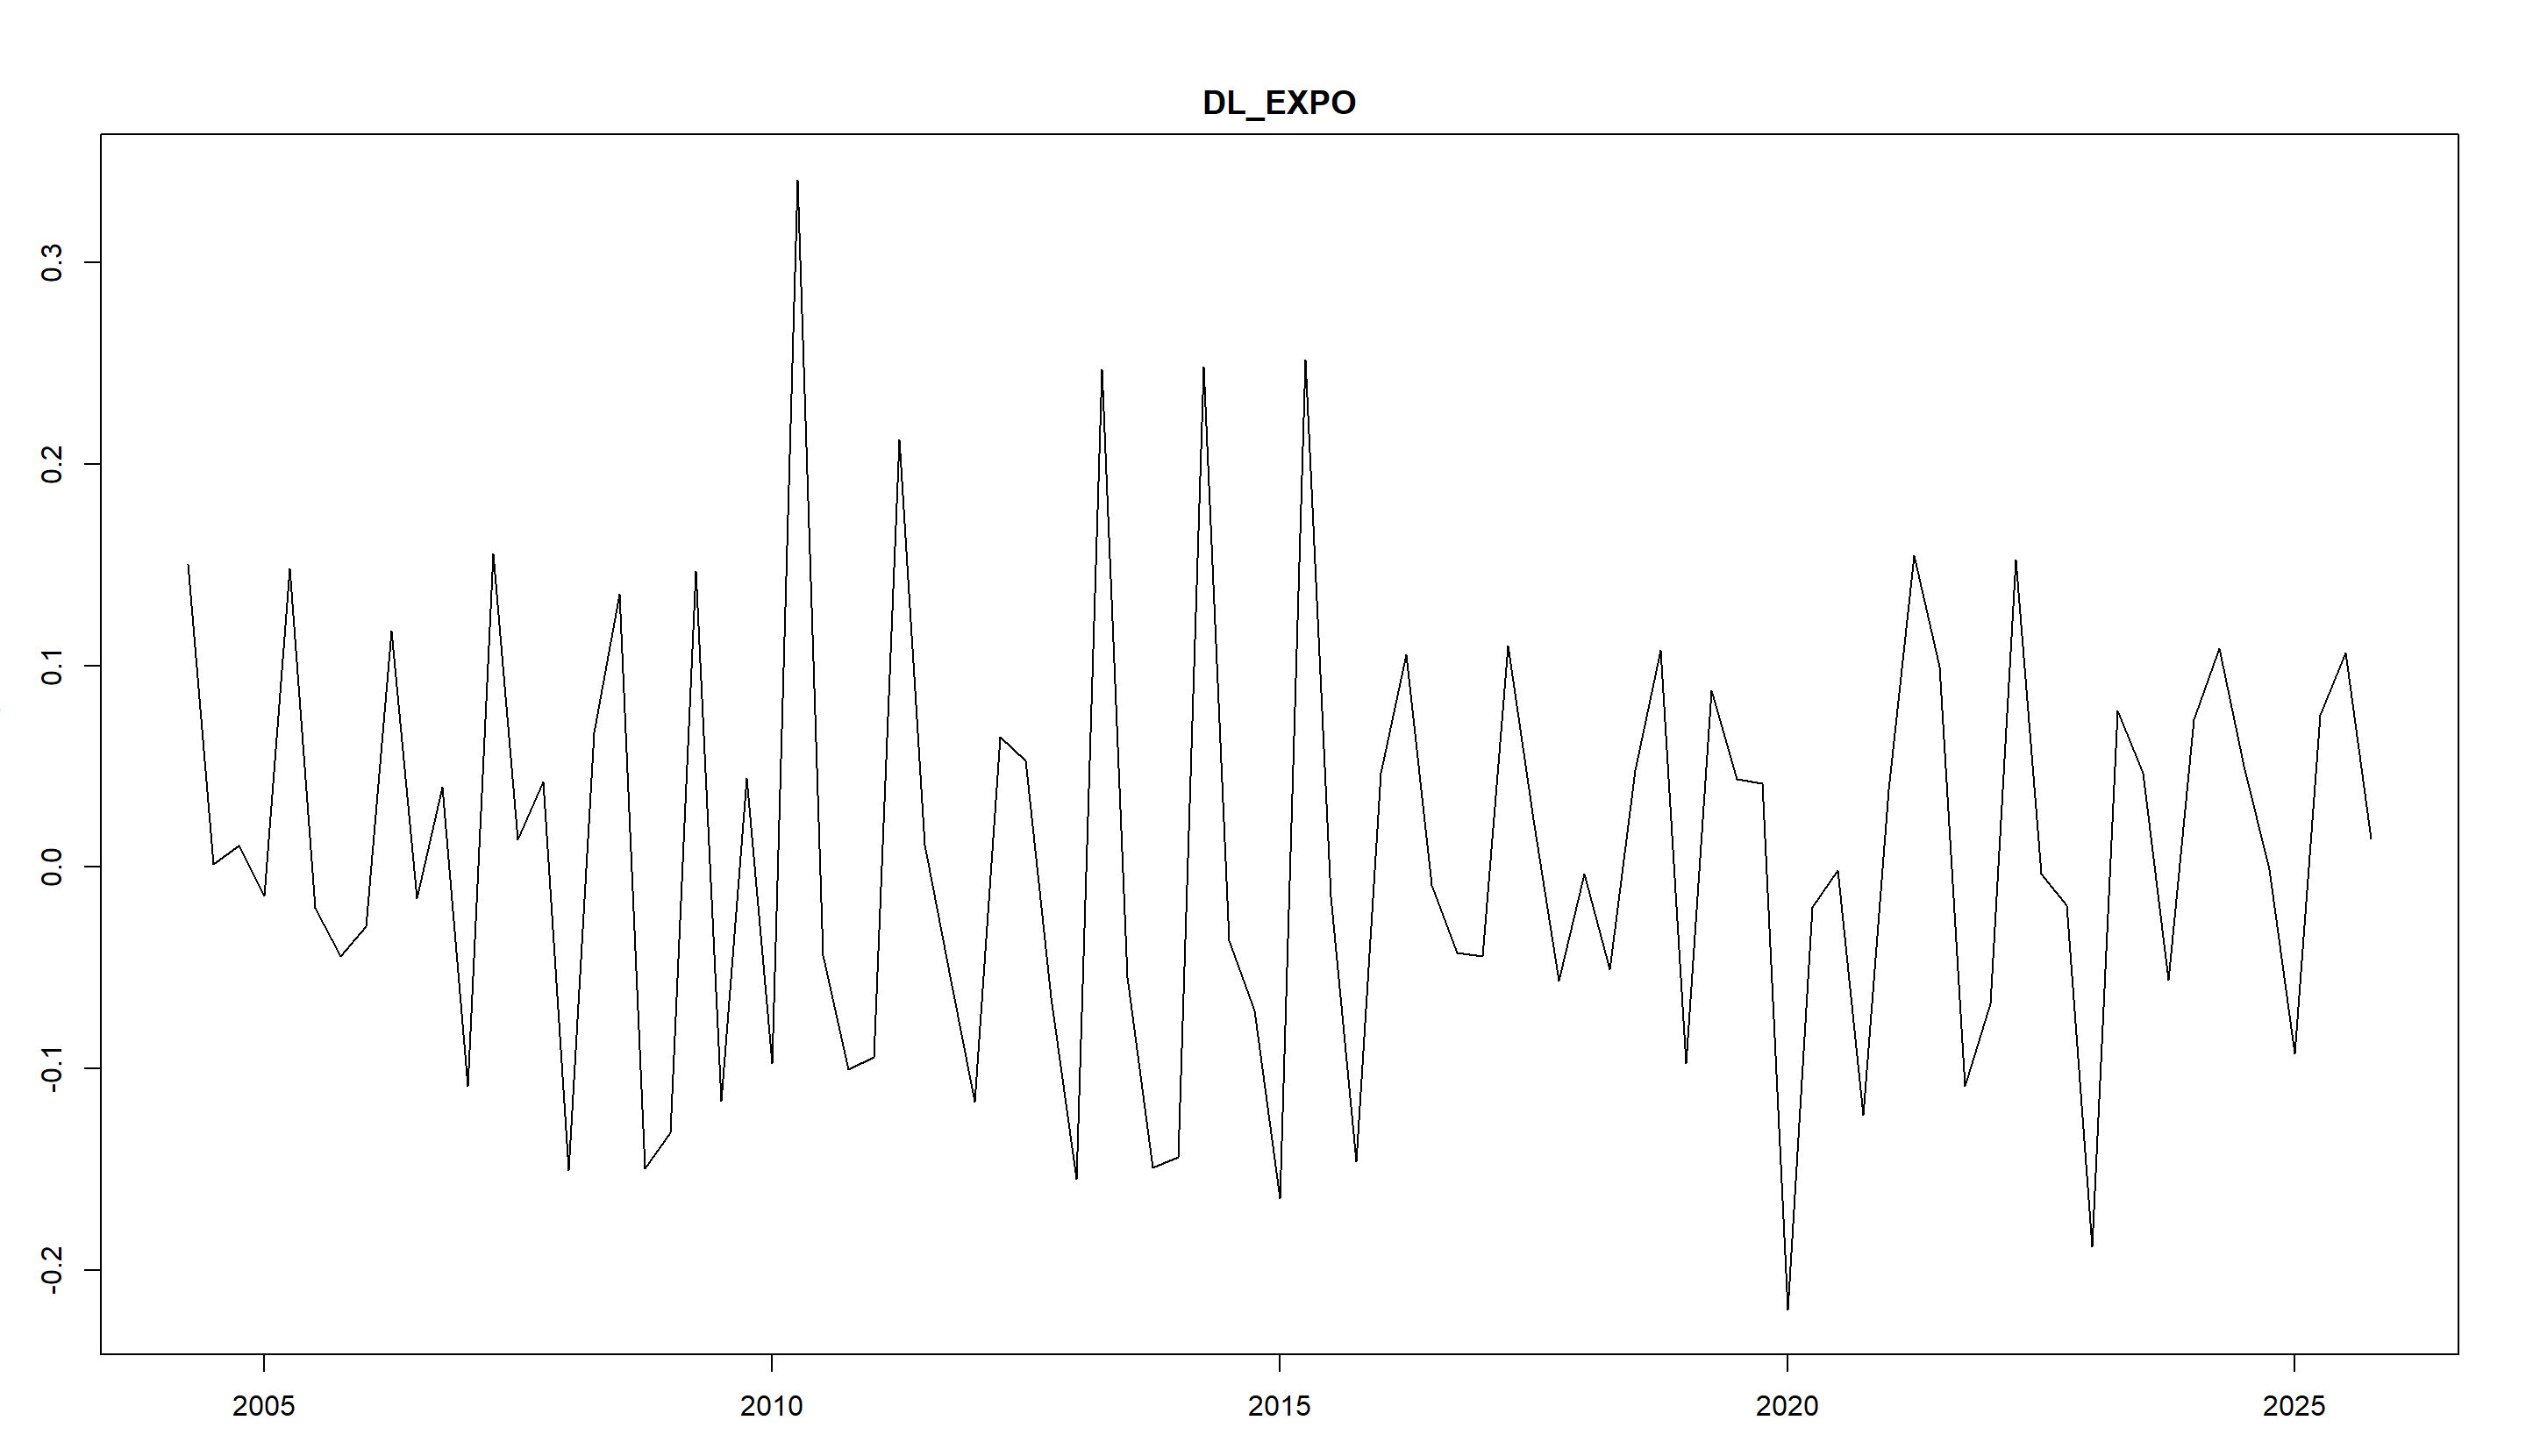
\includegraphics[width=0.8\textwidth]{7.png}
\caption{Evolución de la serie de exportaciones en diferencias logarítmicas (DL\_EXPO).}
\label{fig:dl_expo}
\end{figure}

Las Figuras~\ref{fig:acf_expo} y~\ref{fig:pacf_expo} muestran los correlogramas ACF y PACF de DL\_EXPO. En la ACF se destacan picos positivos y estadísticamente relevantes en rezagos múltiplos de cuatro, lo que constituye una señal clara de estacionalidad trimestral remanente en la serie. Entre esos rezagos también aparecen autocorrelaciones negativas de corto plazo, reflejando una dinámica oscilante. Por su parte, la PACF exhibe coeficientes significativos en los primeros rezagos y un pico positivo en el rezago estacional, patrón compatible con una estructura autorregresiva de bajo orden combinada con un componente estacional. En conjunto, la evidencia gráfica sugiere que la serie requiere especificaciones parsimoniosas, pero capaces de capturar explícitamente la dependencia estacional.

\begin{figure}[H]
\centering
\begin{subfigure}[t]{0.48\textwidth}
\centering
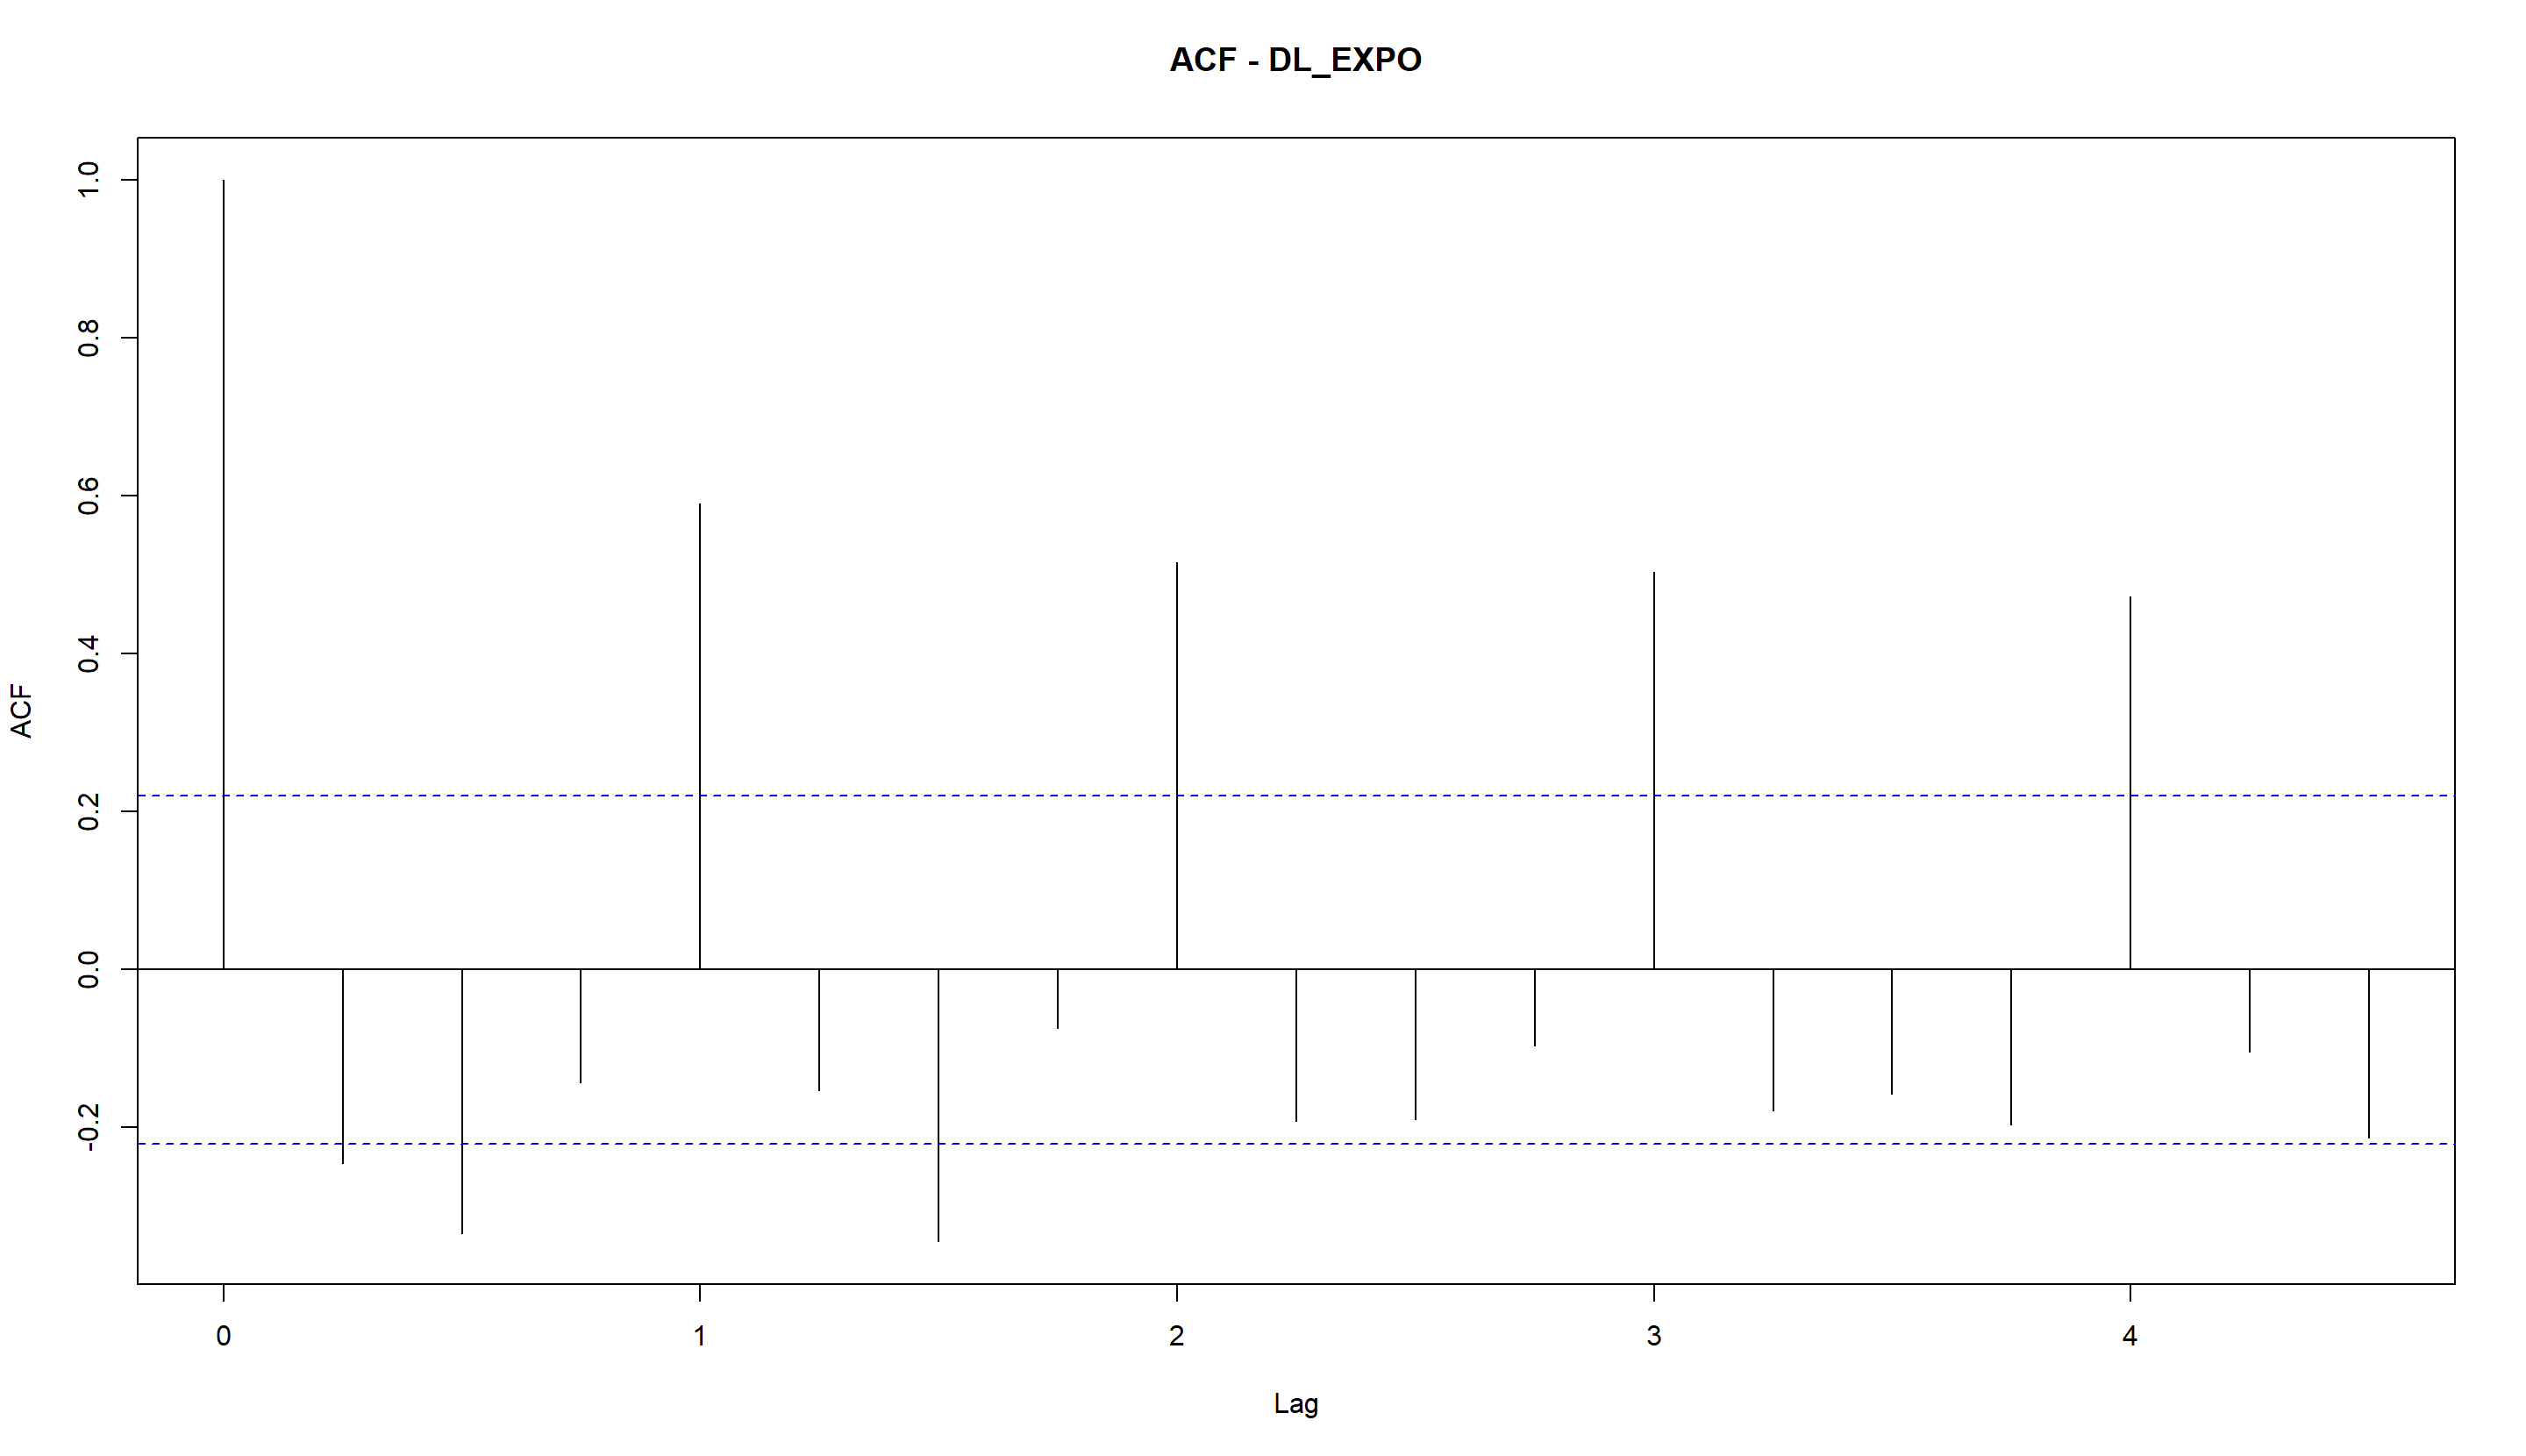
\includegraphics[width=\textwidth]{8.png}
\caption{Función de autocorrelación (ACF) de DL\_EXPO.}
\label{fig:acf_expo}
\end{subfigure}
\hfill
\begin{subfigure}[t]{0.48\textwidth}
\centering
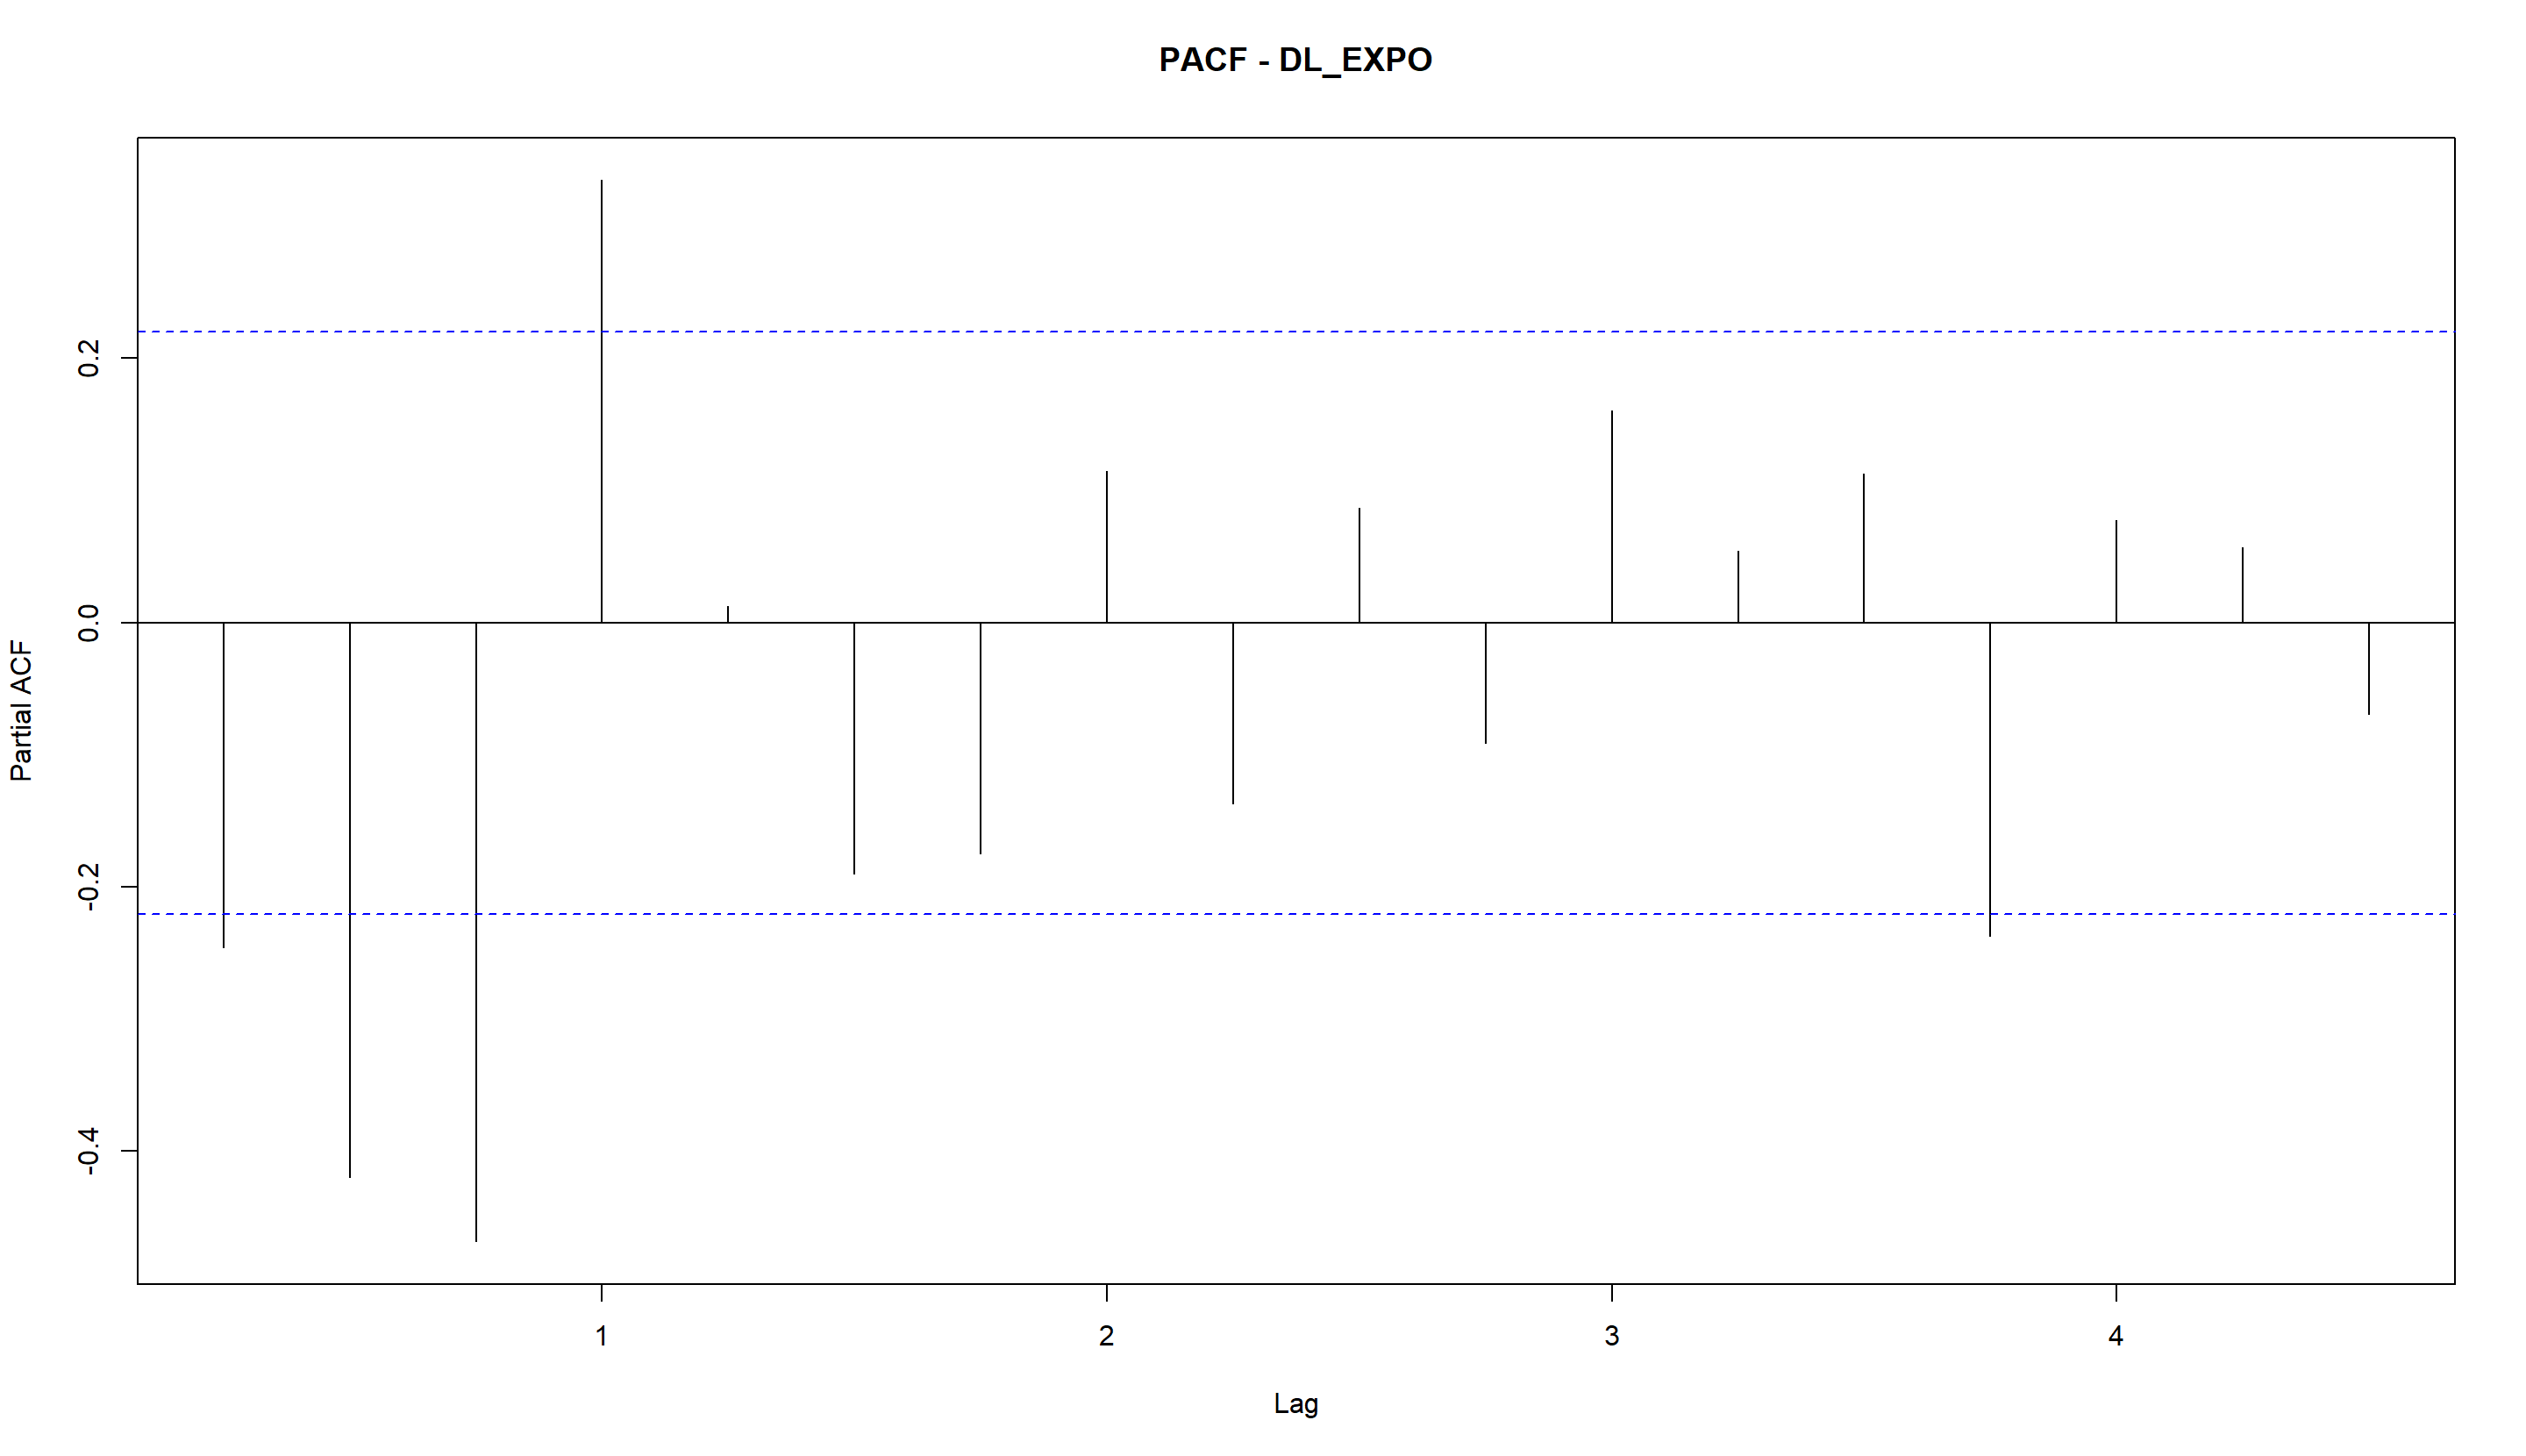
\includegraphics[width=\textwidth]{9.png}
\caption{Función de autocorrelación parcial (PACF) de DL\_EXPO.}
\label{fig:pacf_expo}
\end{subfigure}
\end{figure}

El Cuadro~\ref{tab:sarima_expo} resume la comparación entre las especificaciones SARIMA estimadas sobre la serie original de DL\_EXPO. Los resultados indican que el modelo automático y la especificación SARIMA MA(1) son, en la práctica, indistinguibles: ambos presentan el menor AIC y exactamente los mismos valores de RMSE, MAE, MAPE y autocorrelación residual. Esto sugiere que el procedimiento automático selecciona una estructura muy próxima a una formulación parsimoniosa dominada por un componente de media móvil. En cambio, el modelo SARIMA AR(2) exhibe un AIC menos favorable y un RMSE levemente superior, aunque obtiene un MAE y un MASE marginalmente menores. En conjunto, la evidencia favorece al modelo automático y al MA(1), ya que combinan mejor ajuste global con mayor parsimonia, mientras que la mejora puntual del AR(2) en algunas métricas no alcanza para compensar su peor desempeño relativo en términos de información y error cuadrático.

\begin{table}[H]
\centering
\caption{Comparación de modelos SARIMA – DL\_EXPO}
\label{tab:sarima_expo}
\begin{tabular}{lcccccc}
\hline
Modelo & AIC & RMSE & MAE & MAPE & MASE & ACF (res.) \\
\hline
SARIMA automático & -164.25 & 0.07141 & 0.05375 & 164.59 & 0.69850 & -0.0404 \\
SARIMA MA(1)      & -164.25 & 0.07141 & 0.05375 & 164.59 & 0.69850 & -0.0404 \\
SARIMA AR(2)      & -163.37 & 0.07151 & 0.05333 & 172.80 & 0.69301 & -0.0522 \\
\hline
\end{tabular}
\end{table}

El Cuadro~\ref{tab:diag_expo} presenta los diagnósticos residuales de estas especificaciones. En los tres casos, los p-valores de las pruebas de Ljung-Box y Box-Ljung son superiores a los niveles usuales de significatividad, por lo que no se rechaza la hipótesis nula de ausencia de autocorrelación serial en los residuos. En consecuencia, todas las alternativas resultan admisibles desde el punto de vista del diagnóstico. No obstante, el modelo AR(2) muestra p-valores algo más altos, lo que sugiere una leve mejora en términos de limpieza residual; aun así, esa ventaja diagnóstica es modesta y no modifica la conclusión anterior de que las especificaciones automática y MA(1) constituyen opciones más equilibradas al considerar conjuntamente ajuste, parsimonia y consistencia estadística.

\begin{table}[H]
\centering
\caption{Diagnóstico de residuos – DL\_EXPO}
\label{tab:diag_expo}
\begin{tabular}{lcc}
\hline
Modelo & Ljung-Box (p-valor) & Box-Ljung (p-valor) \\
\hline
SARIMA automático & 0.1421 & 0.3321 \\
SARIMA MA(1)      & 0.1421 & 0.3321 \\
SARIMA AR(2)      & 0.2016 & 0.4950 \\
\hline
\end{tabular}
\end{table}

La Figura~\ref{fig:forecast_expo_sarima} compara los pronósticos fuera de muestra generados por las tres especificaciones SARIMA consideradas para DL\_EXPO. Visualmente, el modelo automático y la variante MA(1) producen trayectorias prácticamente superpuestas, con el mismo perfil oscilante y bandas de confianza muy similares, lo que refuerza la evidencia previa de que ambas especificaciones capturan una dinámica casi idéntica. El modelo AR(2), por su parte, también reproduce la alternancia entre trimestres de expansión y contracción, pero no introduce una mejora sustantiva en el patrón proyectado. En los tres casos, las trayectorias de pronóstico fluctúan alrededor de cero y preservan una oscilación compatible con la estacionalidad observada en la serie, mientras que la amplitud de los intervalos de confianza refleja la elevada volatilidad de las exportaciones y la dificultad inherente para anticipar con precisión sus movimientos de corto plazo.

\begin{figure}[H]
\centering
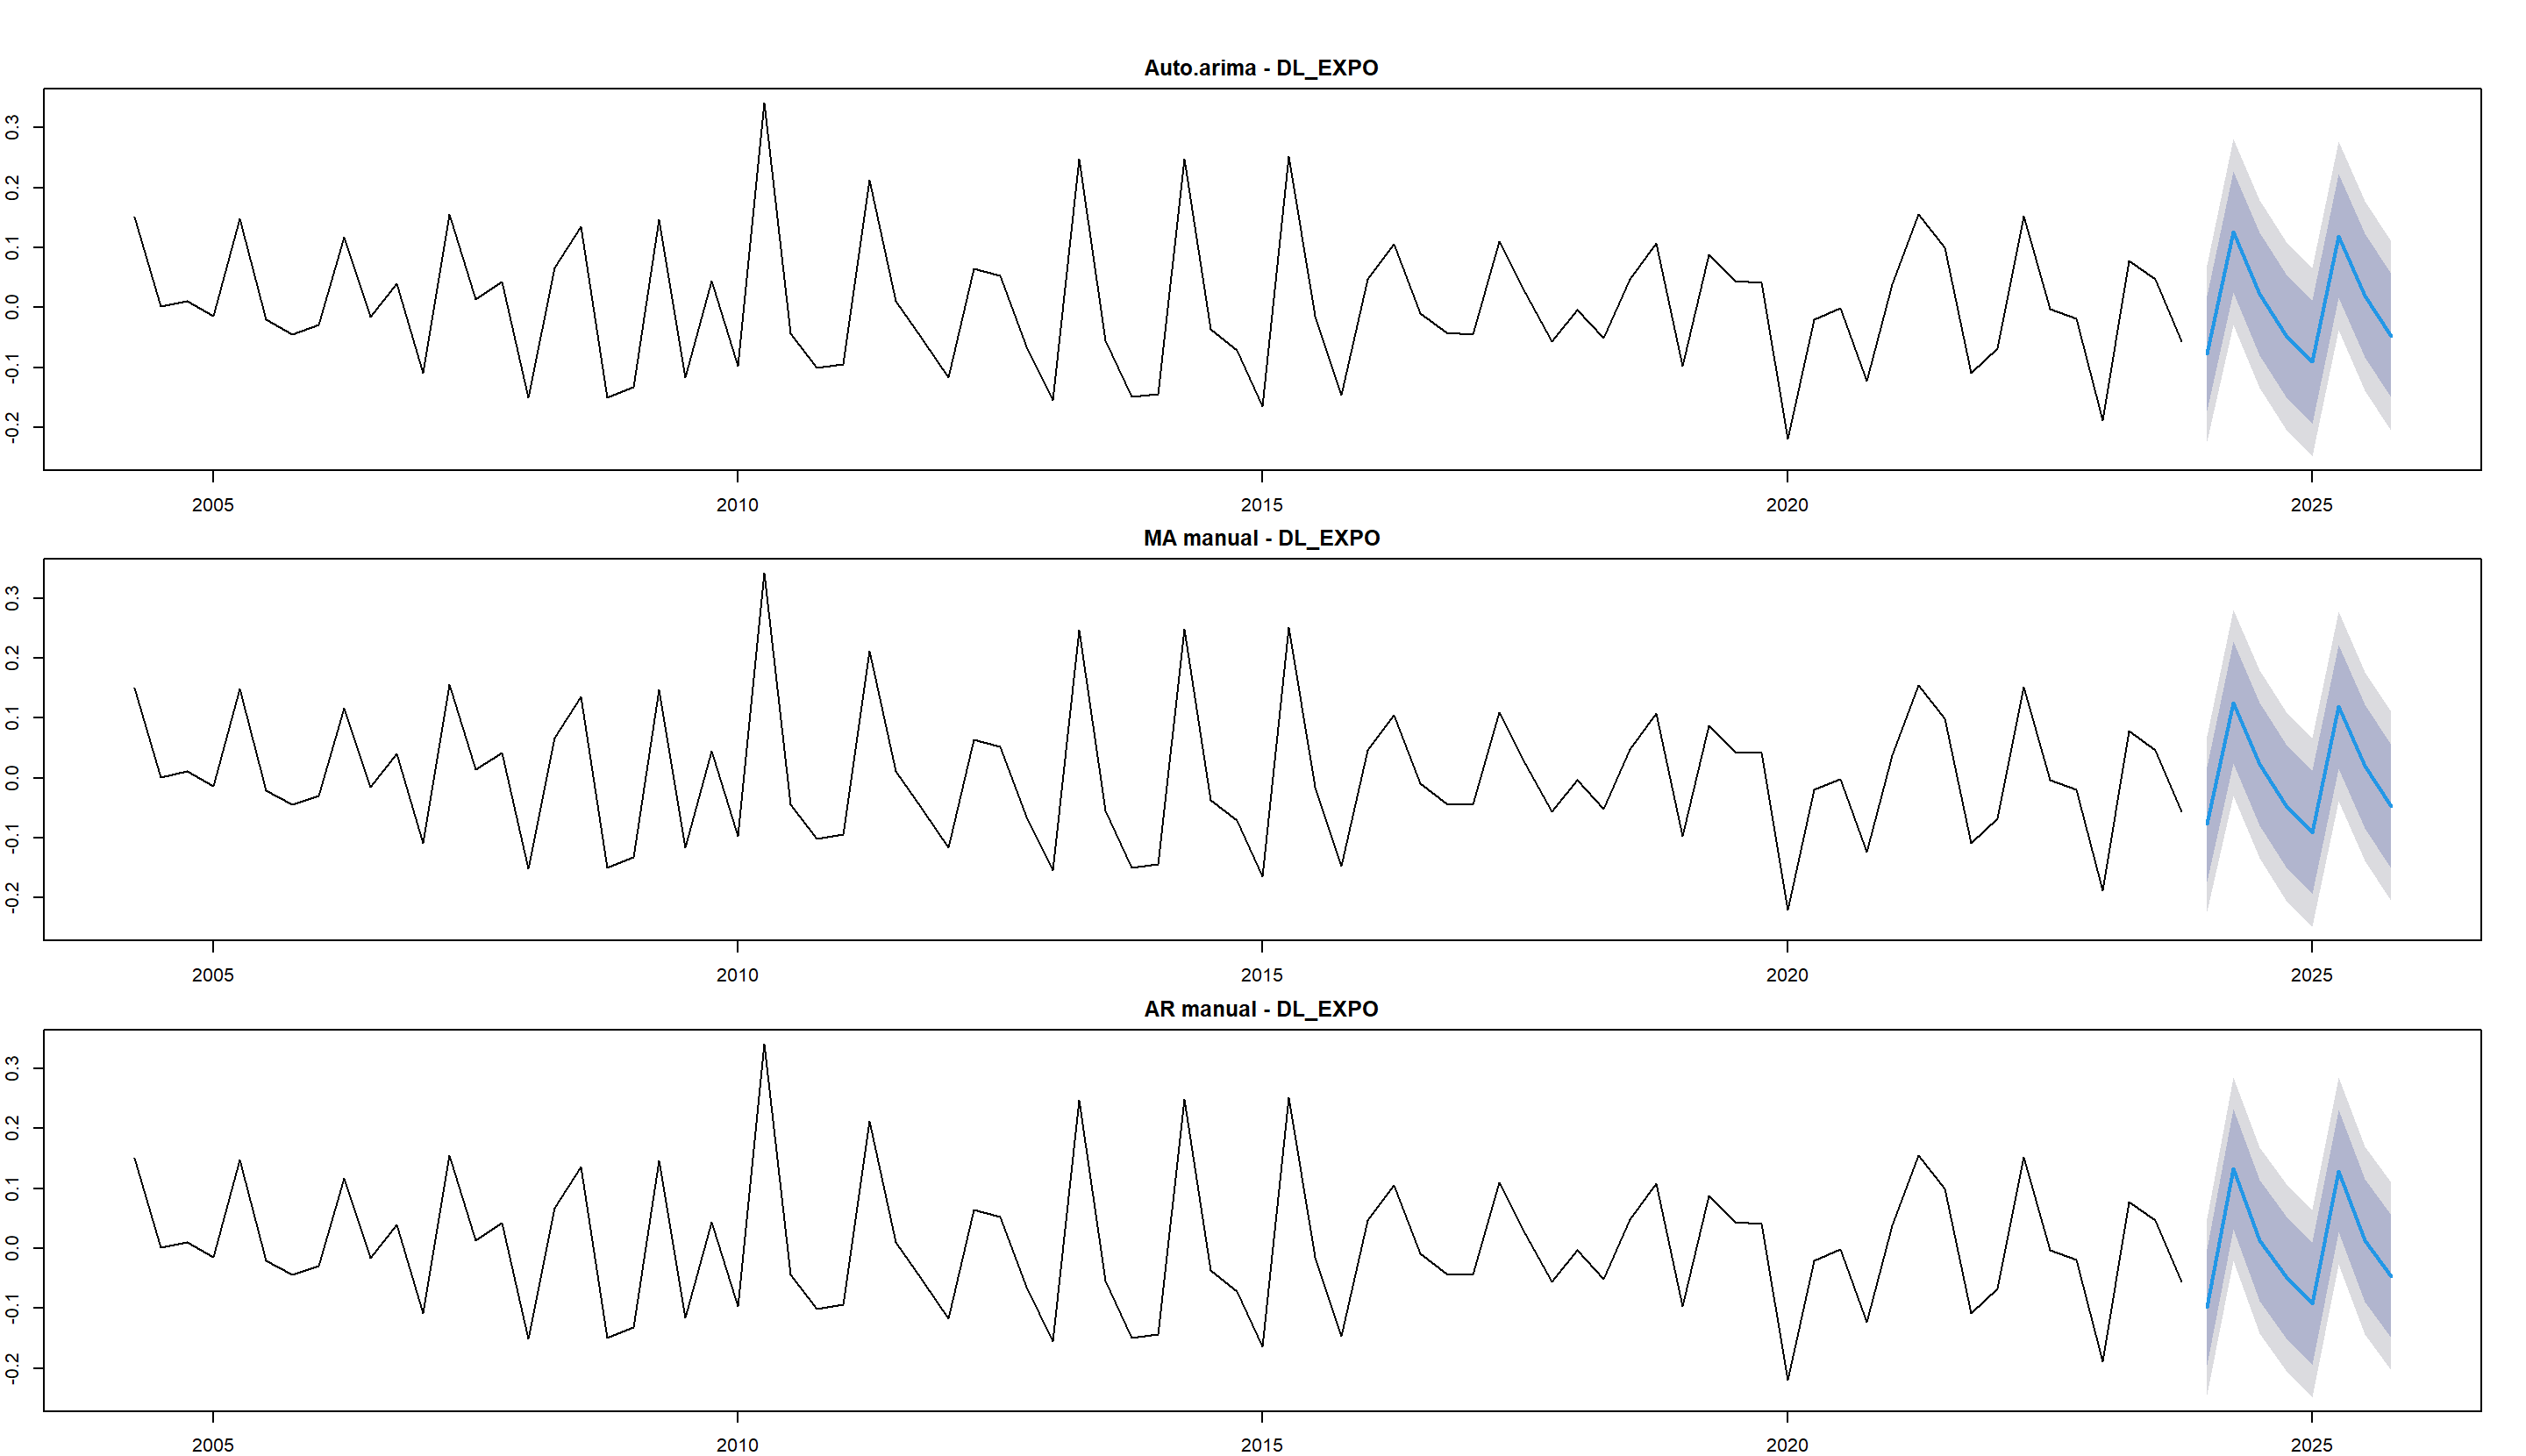
\includegraphics[width=0.9\textwidth]{10.png}
\caption{Comparación de pronósticos para la serie DL\_EXPO utilizando modelos SARIMA: automático, MA(1) y AR(2). La línea azul representa el pronóstico y las bandas sombreadas los intervalos de confianza.}
\label{fig:forecast_expo_sarima}
\end{figure}

El Cuadro~\ref{tab:forecast_expo_sarima} reporta la evaluación del desempeño predictivo fuera de muestra para el período 2024--2025. Los resultados confirman que el modelo SARIMA automático y la especificación MA(1) ofrecen exactamente el mismo desempeño en todas las métricas reportadas, mientras que el modelo AR(2) presenta errores más altos en términos de RMSE, MAE, MAPE y U de Theil. En consecuencia, no hay evidencia de que una estructura autorregresiva más rica mejore la capacidad predictiva de la serie; por el contrario, las especificaciones más parsimoniosas resultan suficientes para capturar la información útil para el pronóstico. La descomposición del coeficiente U de Theil muestra, además, que en los tres modelos la mayor parte del error se concentra en el componente de covarianza, lo que sugiere que las discrepancias provienen principalmente de la dificultad para reproducir con exactitud el timing y la magnitud de las fluctuaciones, más que de un sesgo sistemático en el nivel de las predicciones. Finalmente, el valor elevado del MAPE debe interpretarse con cautela, dado que la serie está expresada en diferencias logarítmicas y toma valores cercanos a cero, circunstancia que tiende a amplificar esta métrica relativa.

\begin{table}[H]
\centering
\caption{Evaluación de pronósticos – DL\_EXPO}
\label{tab:forecast_expo_sarima}
\begin{tabular}{lccc}
\hline
Métrica & SARIMA Auto & SARIMA MA(1) & SARIMA AR(2) \\
\hline
RMSE         & 0.06972 & 0.06972 & 0.07794 \\
MAE          & 0.05436 & 0.05436 & 0.06084 \\
MAPE         & 551.50  & 551.50  & 571.31 \\
U de Theil   & 0.45292 & 0.45292 & 0.48760 \\
U sesgo      & 0.30407 & 0.30407 & 0.27854 \\
U varianza   & 0.05184 & 0.05184 & 0.07856 \\
U covarianza & 0.64409 & 0.64409 & 0.64290 \\
\hline
\end{tabular}
\end{table}

La Figura~\ref{fig:dl_expo_sa} presenta la serie DL\_EXPO una vez removido el componente estacional mediante el procedimiento X-13. En comparación con la serie original, la trayectoria desestacionalizada conserva la volatilidad característica de las exportaciones, pero exhibe fluctuaciones más concentradas alrededor de cero y una oscilación menos claramente asociada al patrón trimestral regular. Aun así, persisten episodios de variación abrupta en distintos momentos de la muestra, lo que sugiere que la desestacionalización elimina una parte importante de la periodicidad sistemática, aunque no suprime la sensibilidad de la serie a shocks transitorios y a cambios bruscos en el entorno económico. En este sentido, la serie ajustada ofrece una base más limpia para identificar la dinámica no estacional y evaluar si una especificación ARMA simple resulta suficiente para describirla.

\begin{figure}[H]
\centering
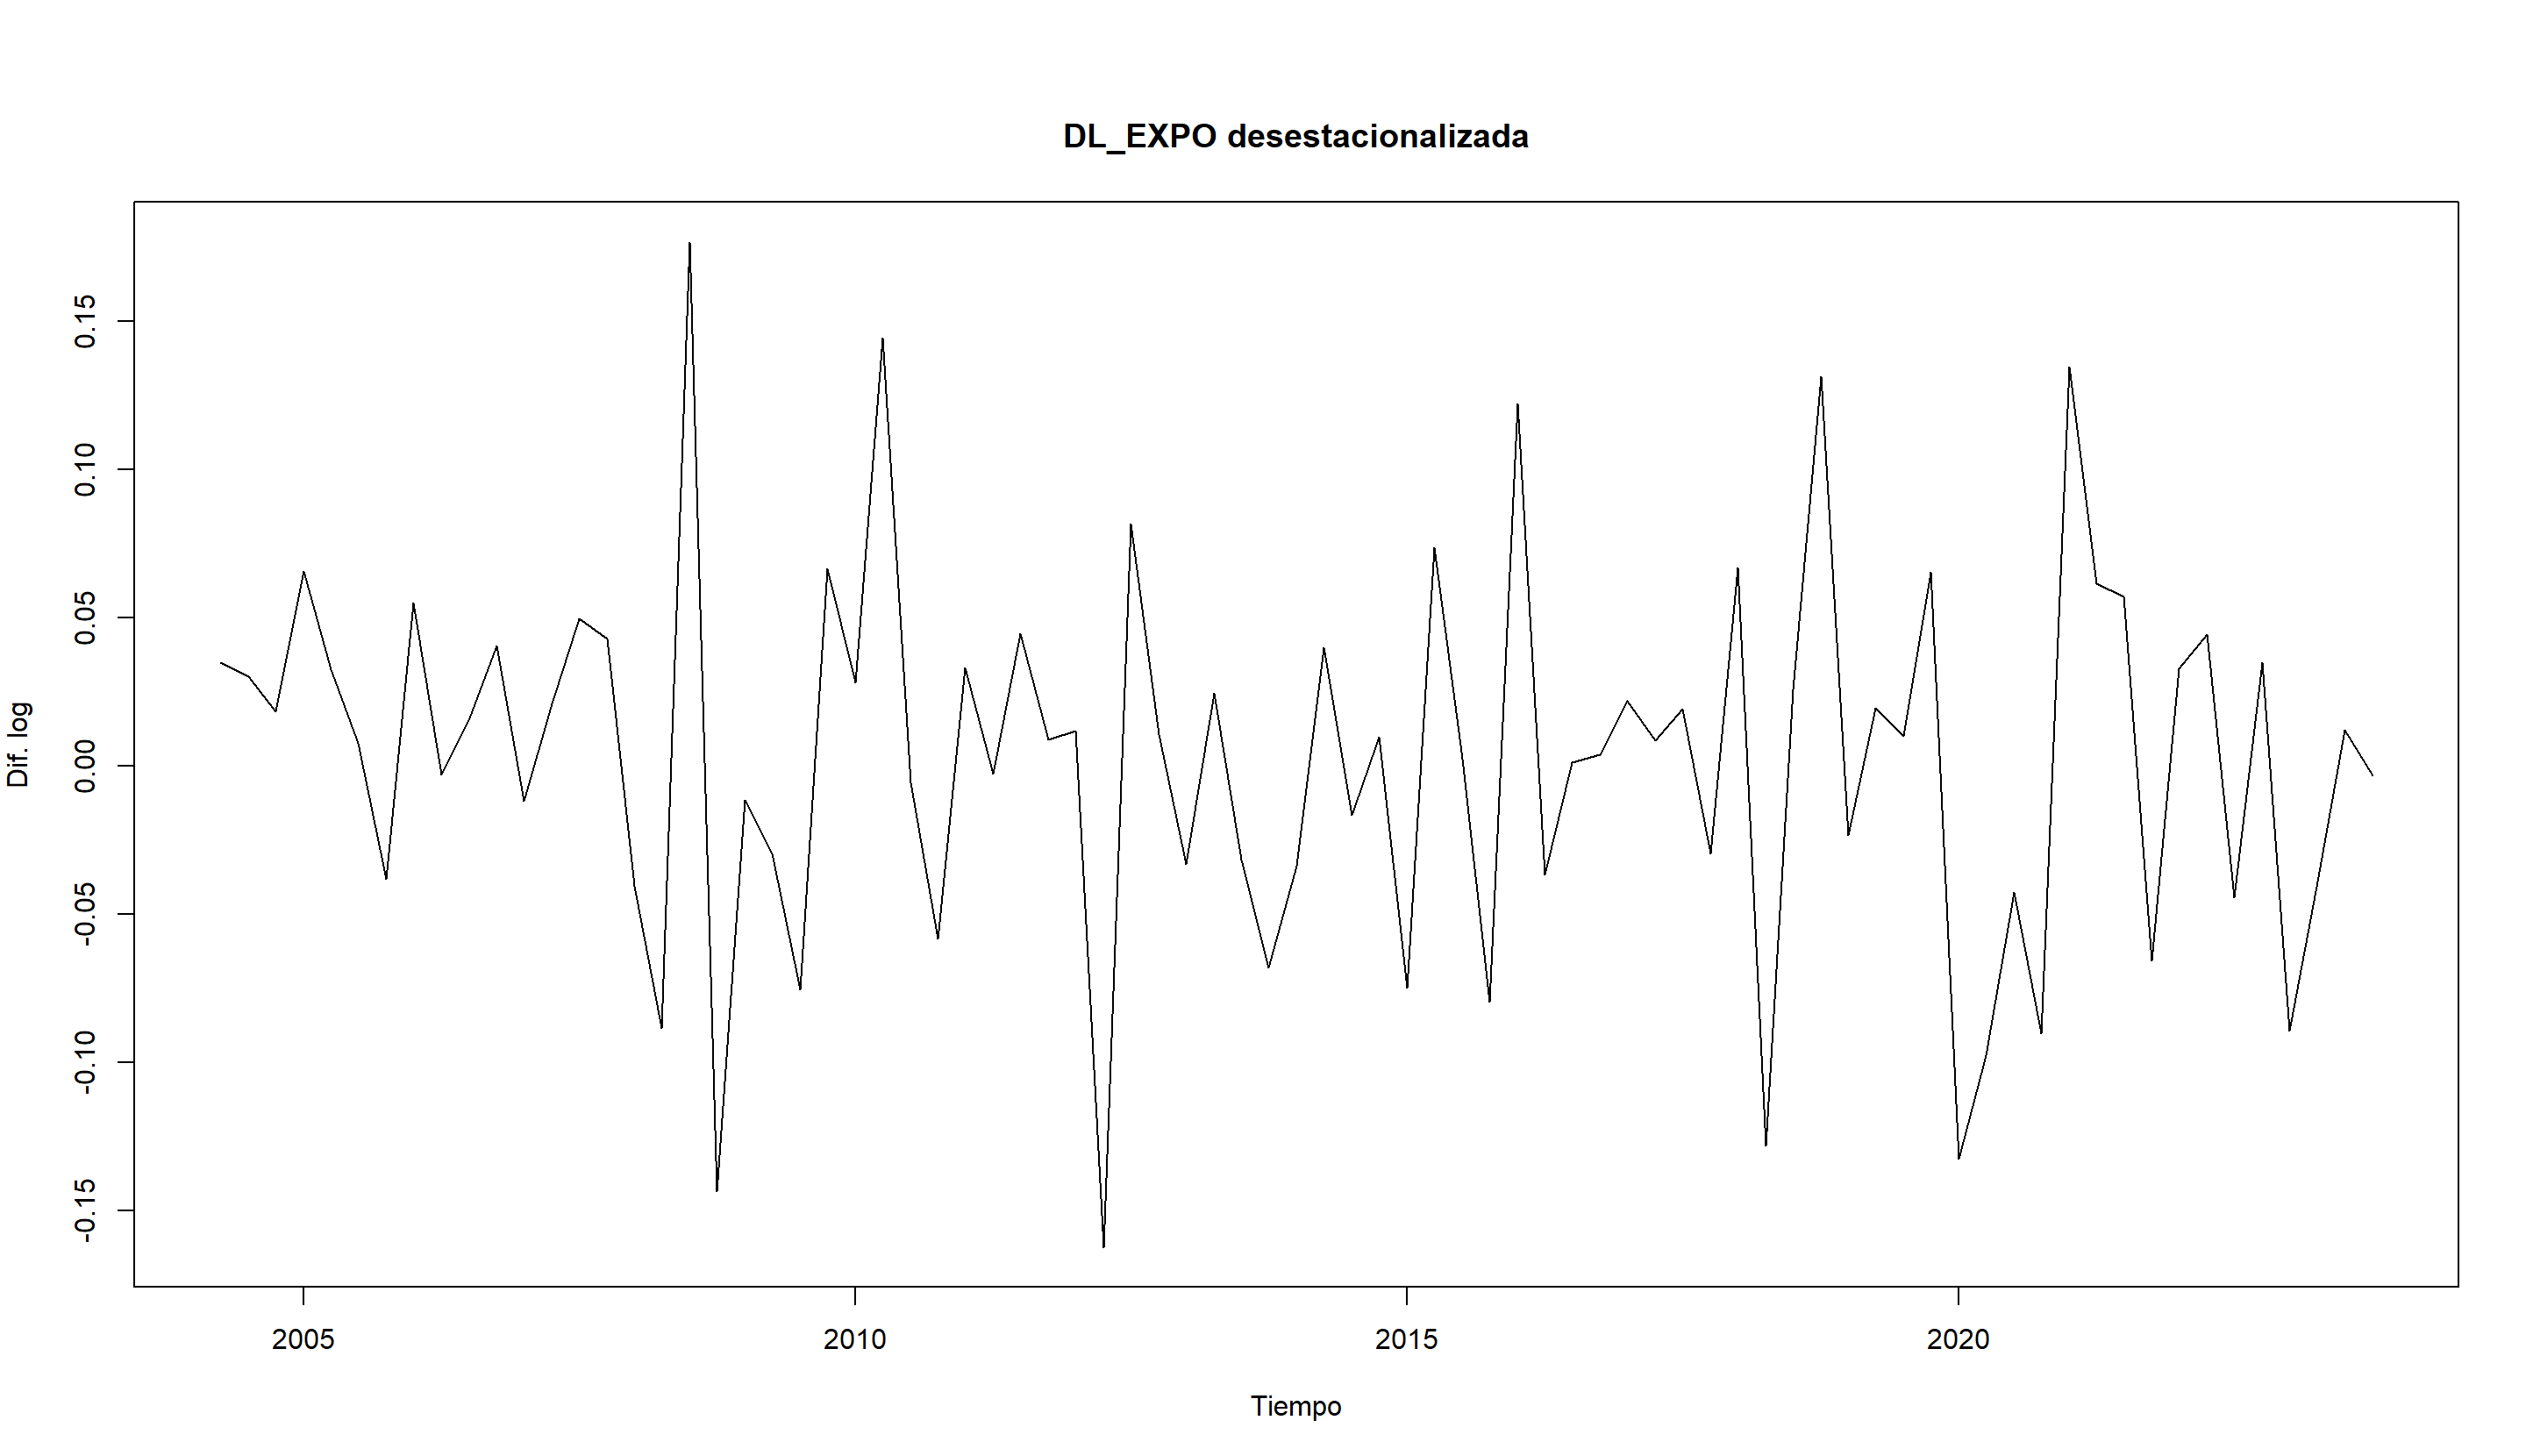
\includegraphics[width=0.9\textwidth]{11.png}
\caption{Serie DL\_EXPO desestacionalizada mediante X-13}
\label{fig:dl_expo_sa}
\end{figure}

Las Figuras~\ref{fig:acf_expo_sa} y~\ref{fig:pacf_expo_sa} muestran los correlogramas de la serie desestacionalizada. A diferencia de lo observado en la serie original, la ACF ya no exhibe picos positivos pronunciados y repetidos en rezagos múltiplos de cuatro, lo que indica que la regularidad estacional ha sido sustancialmente removida. La mayor parte de las autocorrelaciones se ubica dentro de las bandas de significatividad, con apenas algunos rezagos aislados que sugieren dependencia serial débil. De manera consistente, la PACF presenta una estructura dispersa, sin un patrón estacional nítido, aunque con algunos coeficientes individuales que podrían justificar la consideración de modelos de bajo orden. En conjunto, la evidencia gráfica sugiere que, una vez desestacionalizada la serie, la dinámica remanente de DL\_EXPO es más tenue y puede ser razonablemente aproximada mediante especificaciones parsimoniosas, en particular con componentes de media móvil o combinaciones ARMA simples.

\begin{figure}[H]
\centering
\begin{subfigure}[t]{0.48\textwidth}
\centering
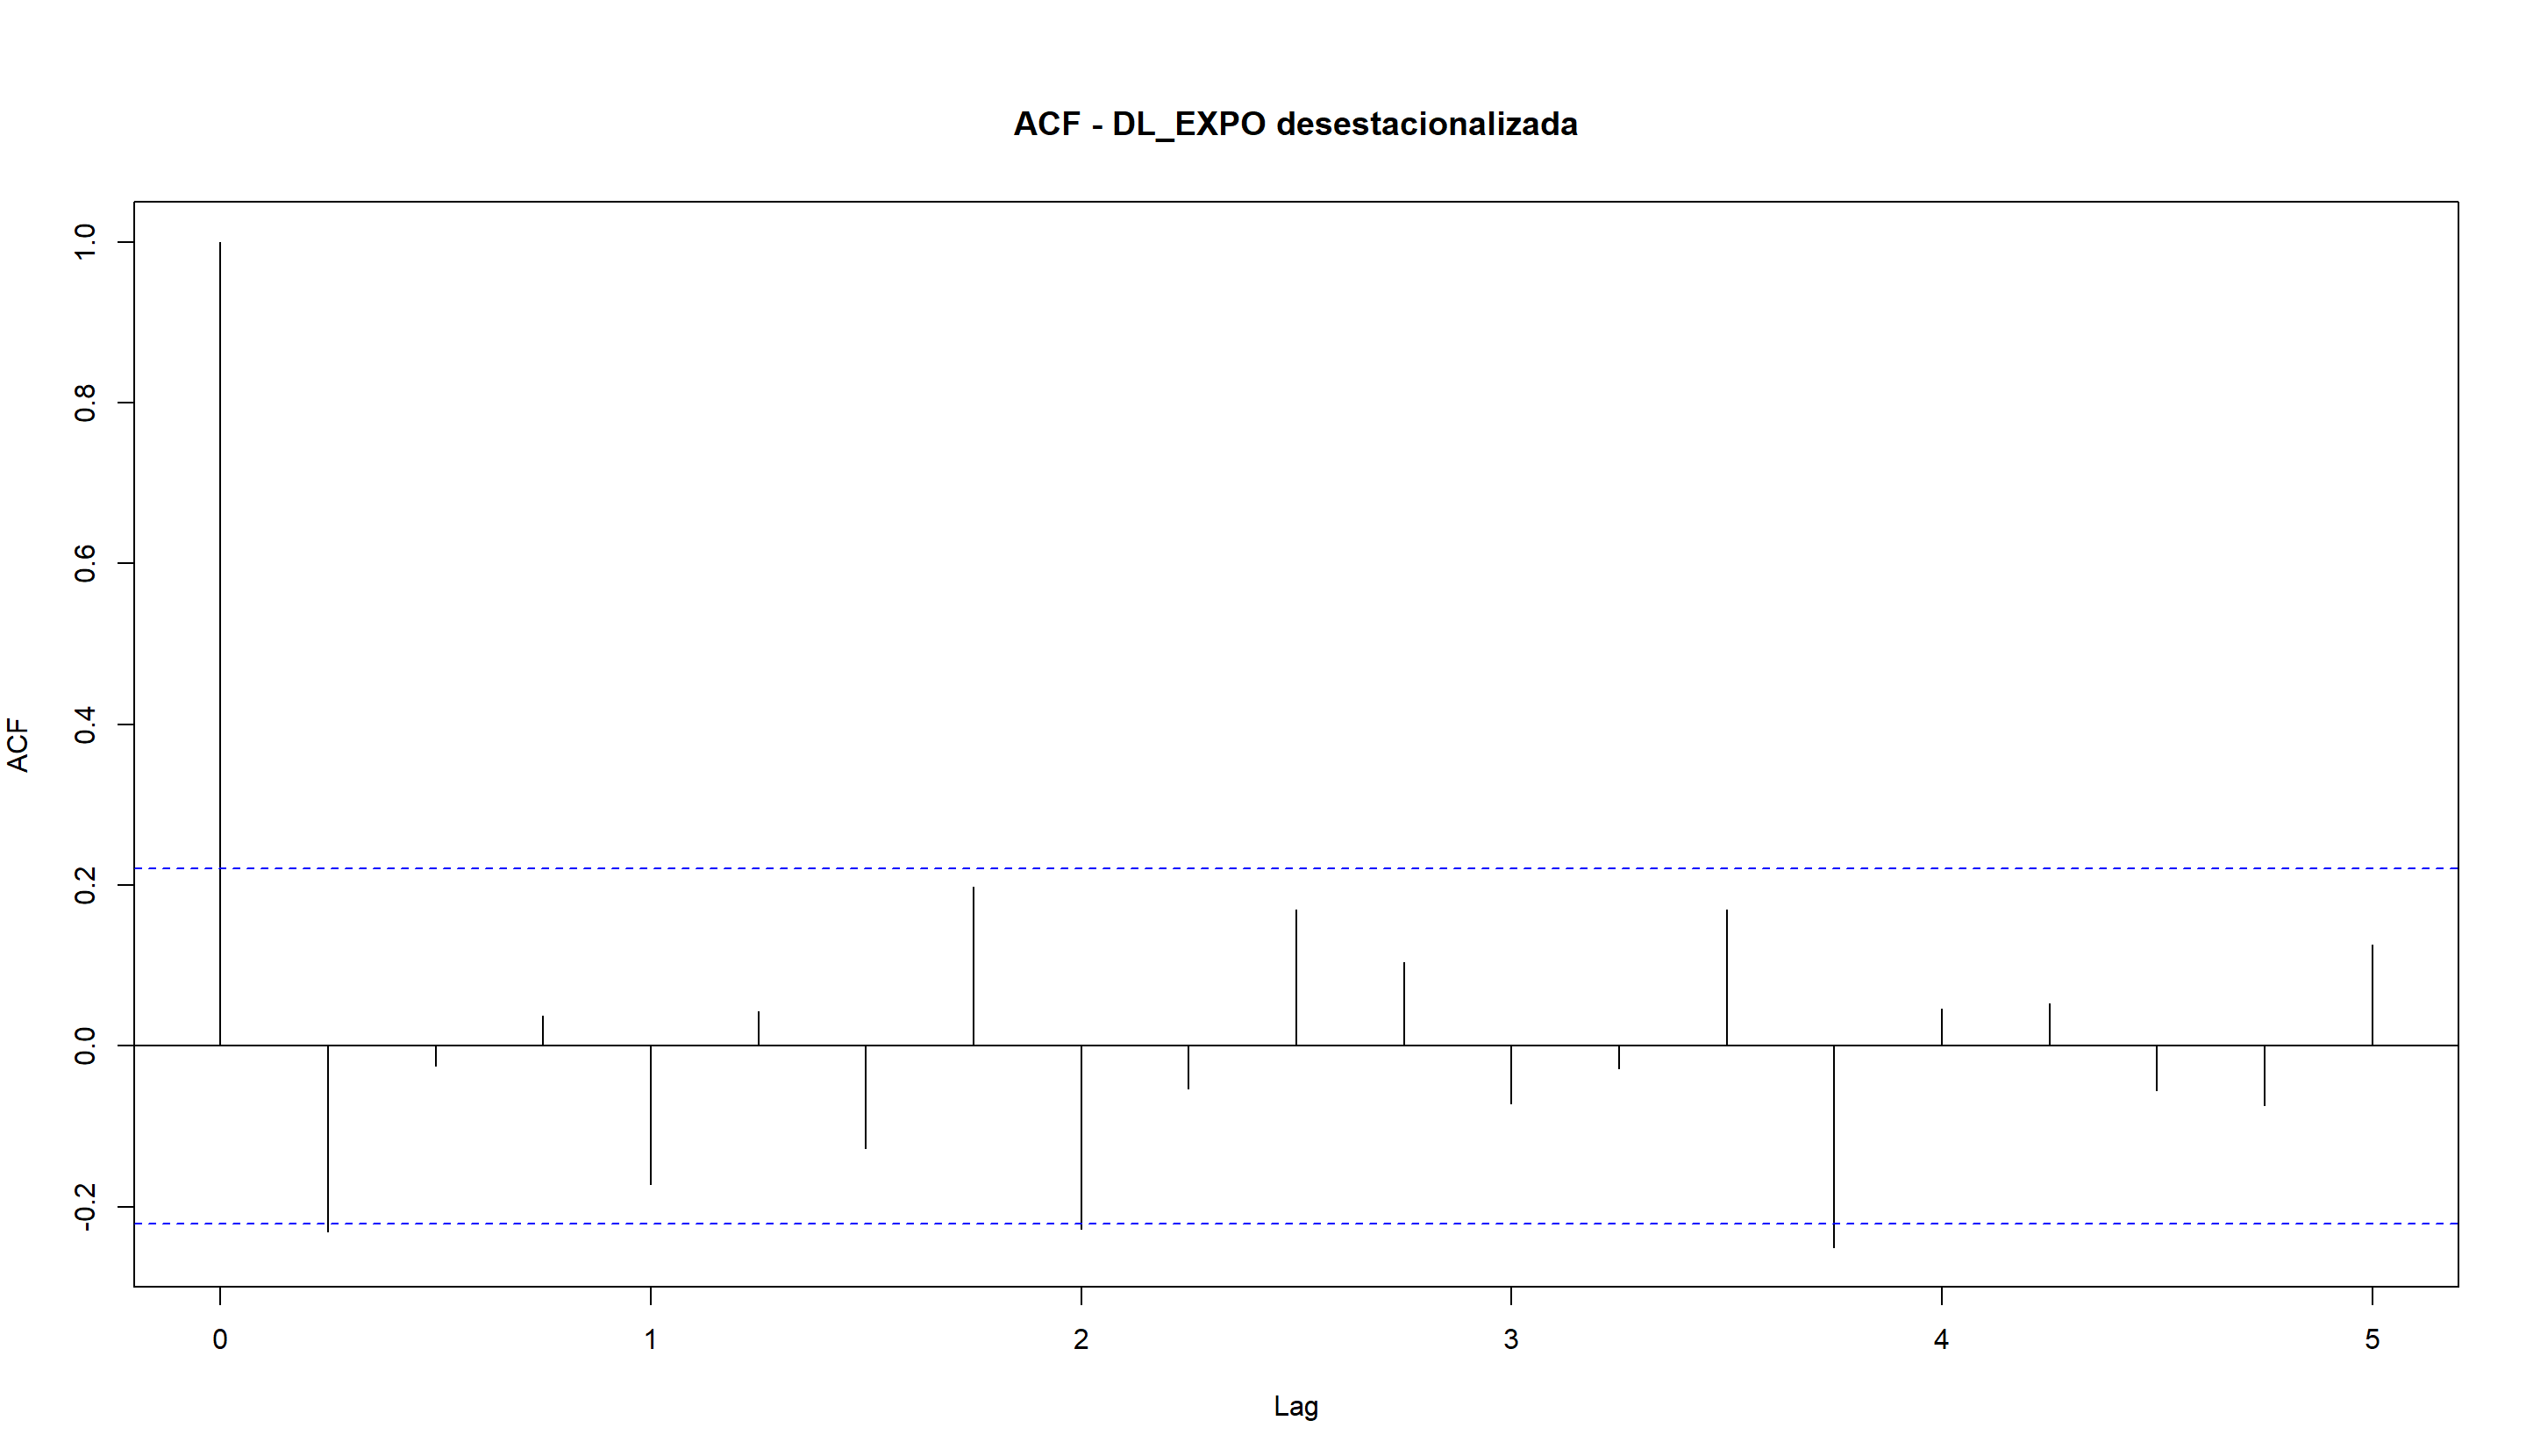
\includegraphics[width=\textwidth]{12.png}
\caption{Función de autocorrelación (ACF) de la serie DL\_EXPO desestacionalizada.}
\label{fig:acf_expo_sa}
\end{subfigure}
\hfill
\begin{subfigure}[t]{0.48\textwidth}
\centering
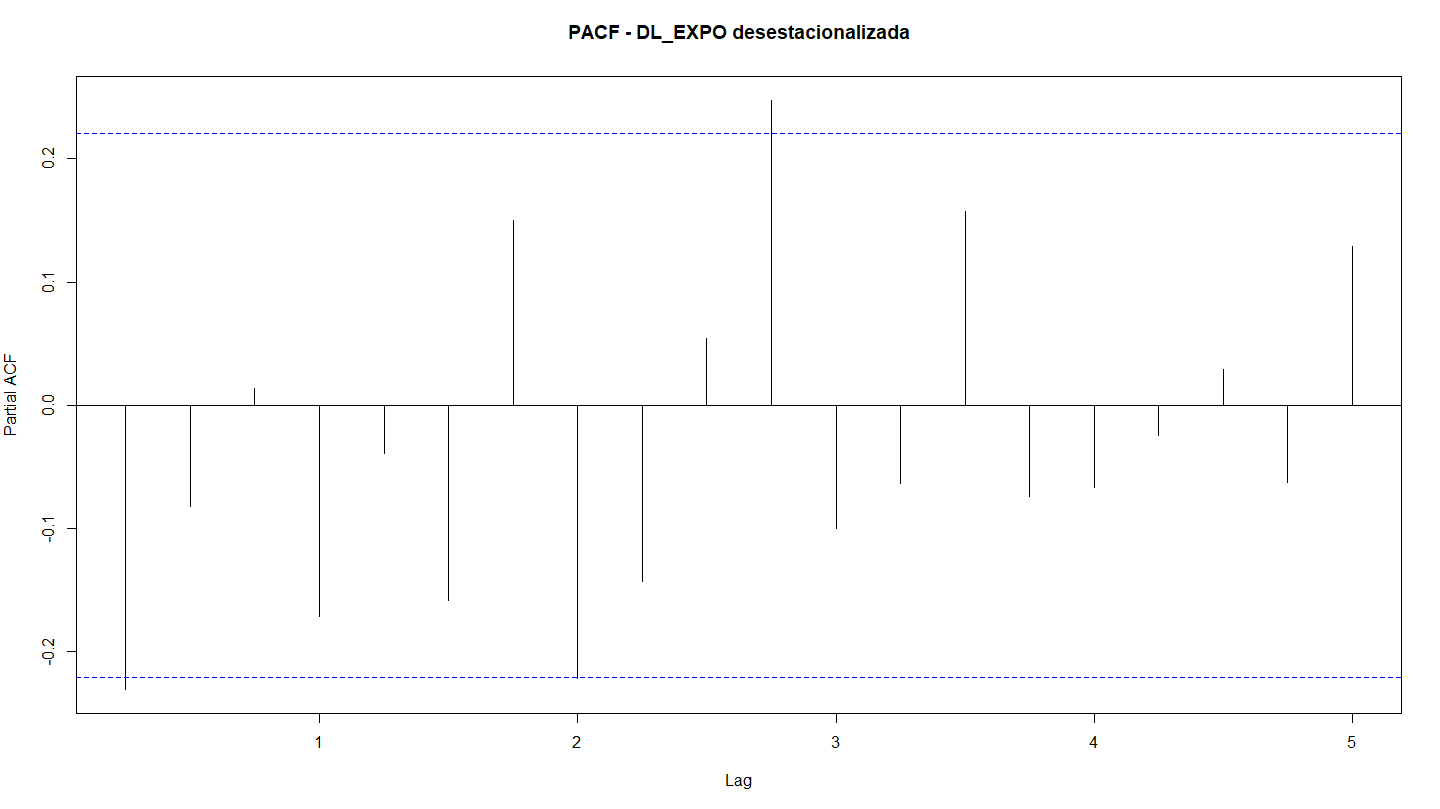
\includegraphics[width=\textwidth]{13.png}
\caption{Función de autocorrelación parcial (PACF) de la serie DL\_EXPO desestacionalizada.}
\label{fig:pacf_expo_sa}
\end{subfigure}
\end{figure}

El Cuadro~\ref{tab:modelos_sa_expo} resume la comparación entre los modelos estimados sobre la serie desestacionalizada de DL\_EXPO. Un primer resultado relevante es que el modelo automático coincide exactamente con un ARIMA(0,0,1) sin media, lo que sugiere que, una vez removido el componente estacional, la dinámica remanente de las exportaciones puede representarse de manera razonable mediante una estructura muy parsimoniosa de media móvil de primer orden. La versión con media presenta un AIC y un BIC menos favorables, de modo que resulta penalizada por su mayor complejidad; sin embargo, exhibe mejoras marginales en RMSE, MAE, MAPE y MASE. En consecuencia, el cuadro muestra una tensión similar a la observada en otras series: si el criterio principal es la parsimonia y la selección por información, las especificaciones sin media resultan preferibles; si se privilegia exclusivamente una mejora cuantitativa, aunque muy pequeña, en las métricas de ajuste, la versión con media aparece apenas por encima. En cualquier caso, las diferencias son reducidas, lo que indica que la desestacionalización deja una dinámica relativamente simple y de baja persistencia.

\begin{table}[H]
\centering
\caption{Comparación de modelos sobre la serie DL\_EXPO desestacionalizada}
\label{tab:modelos_sa_expo}
\begin{tabular}{lcccccc}
\hline
Modelo & AIC & BIC & RMSE & MAE & MAPE & MASE \\
\hline
ARIMA(0,0,1) sin media (Auto) & -210.35 & -205.61 & 0.06229 & 0.04856 & 123.30 & 0.62546 \\
ARIMA(0,0,1) sin media (MA1)  & -210.35 & -205.61 & 0.06229 & 0.04856 & 123.30 & 0.62546 \\
ARIMA(0,0,1) con media        & -208.58 & -201.47 & 0.06219 & 0.04797 & 119.88 & 0.61790 \\
\hline
\end{tabular}
\end{table}

El Cuadro~\ref{tab:diag_sa_expo} presenta los diagnósticos residuales de estas especificaciones. Los p-valores de las pruebas de Ljung-Box y Box-Ljung son superiores a los niveles usuales de significatividad en los tres casos, por lo que no hay evidencia estadística de autocorrelación serial remanente en los residuos. Esto implica que todas las alternativas resultan admisibles desde el punto de vista del diagnóstico y que la desestacionalización logra simplificar la estructura temporal sin dejar patrones residuales importantes. La especificación con media muestra p-valores apenas superiores a los de las variantes sin media, pero la diferencia es mínima y no altera la conclusión general. Por lo tanto, el diagnóstico residual refuerza la idea de que, para DL\_EXPO desestacionalizada, modelos muy simples son suficientes para capturar adecuadamente la dependencia temporal restante.

\begin{table}[H]
\centering
\caption{Diagnóstico de residuos – DL\_EXPO desestacionalizada}
\label{tab:diag_sa_expo}
\begin{tabular}{lcc}
\hline
Modelo & Ljung-Box (p-valor) & Box-Ljung (p-valor) \\
\hline
ARIMA(0,0,1) sin media (Auto) & 0.2373 & 0.2480 \\
ARIMA(0,0,1) sin media (MA1)  & 0.2373 & 0.2480 \\
ARIMA(0,0,1) con media        & 0.2395 & 0.2492 \\
\hline
\end{tabular}
\end{table}

La Figura~\ref{fig:forecast_expo_ma1} compara los pronósticos fuera de muestra obtenidos a partir de los modelos estimados sobre la serie desestacionalizada de DL\_EXPO. Visualmente, las tres trayectorias reproducen una dinámica muy similar y logran captar la alternancia entre valores positivos y negativos observada en el período de prueba, lo que confirma que la parte no estacional de la serie puede modelizarse con estructuras simples. Sin embargo, también se advierte que ninguno de los modelos logra replicar con total precisión la amplitud de todos los movimientos observados, especialmente en los cambios más abruptos entre trimestres, lo que es consistente con la elevada volatilidad propia de las exportaciones. Entre las alternativas consideradas, la especificación MA(1) con media muestra una trayectoria levemente más cercana a los valores efectivos en varios puntos del horizonte de pronóstico, mientras que el modelo automático y el MA(1) sin media generan perfiles prácticamente indistinguibles entre sí.

\begin{figure}[H]
\centering
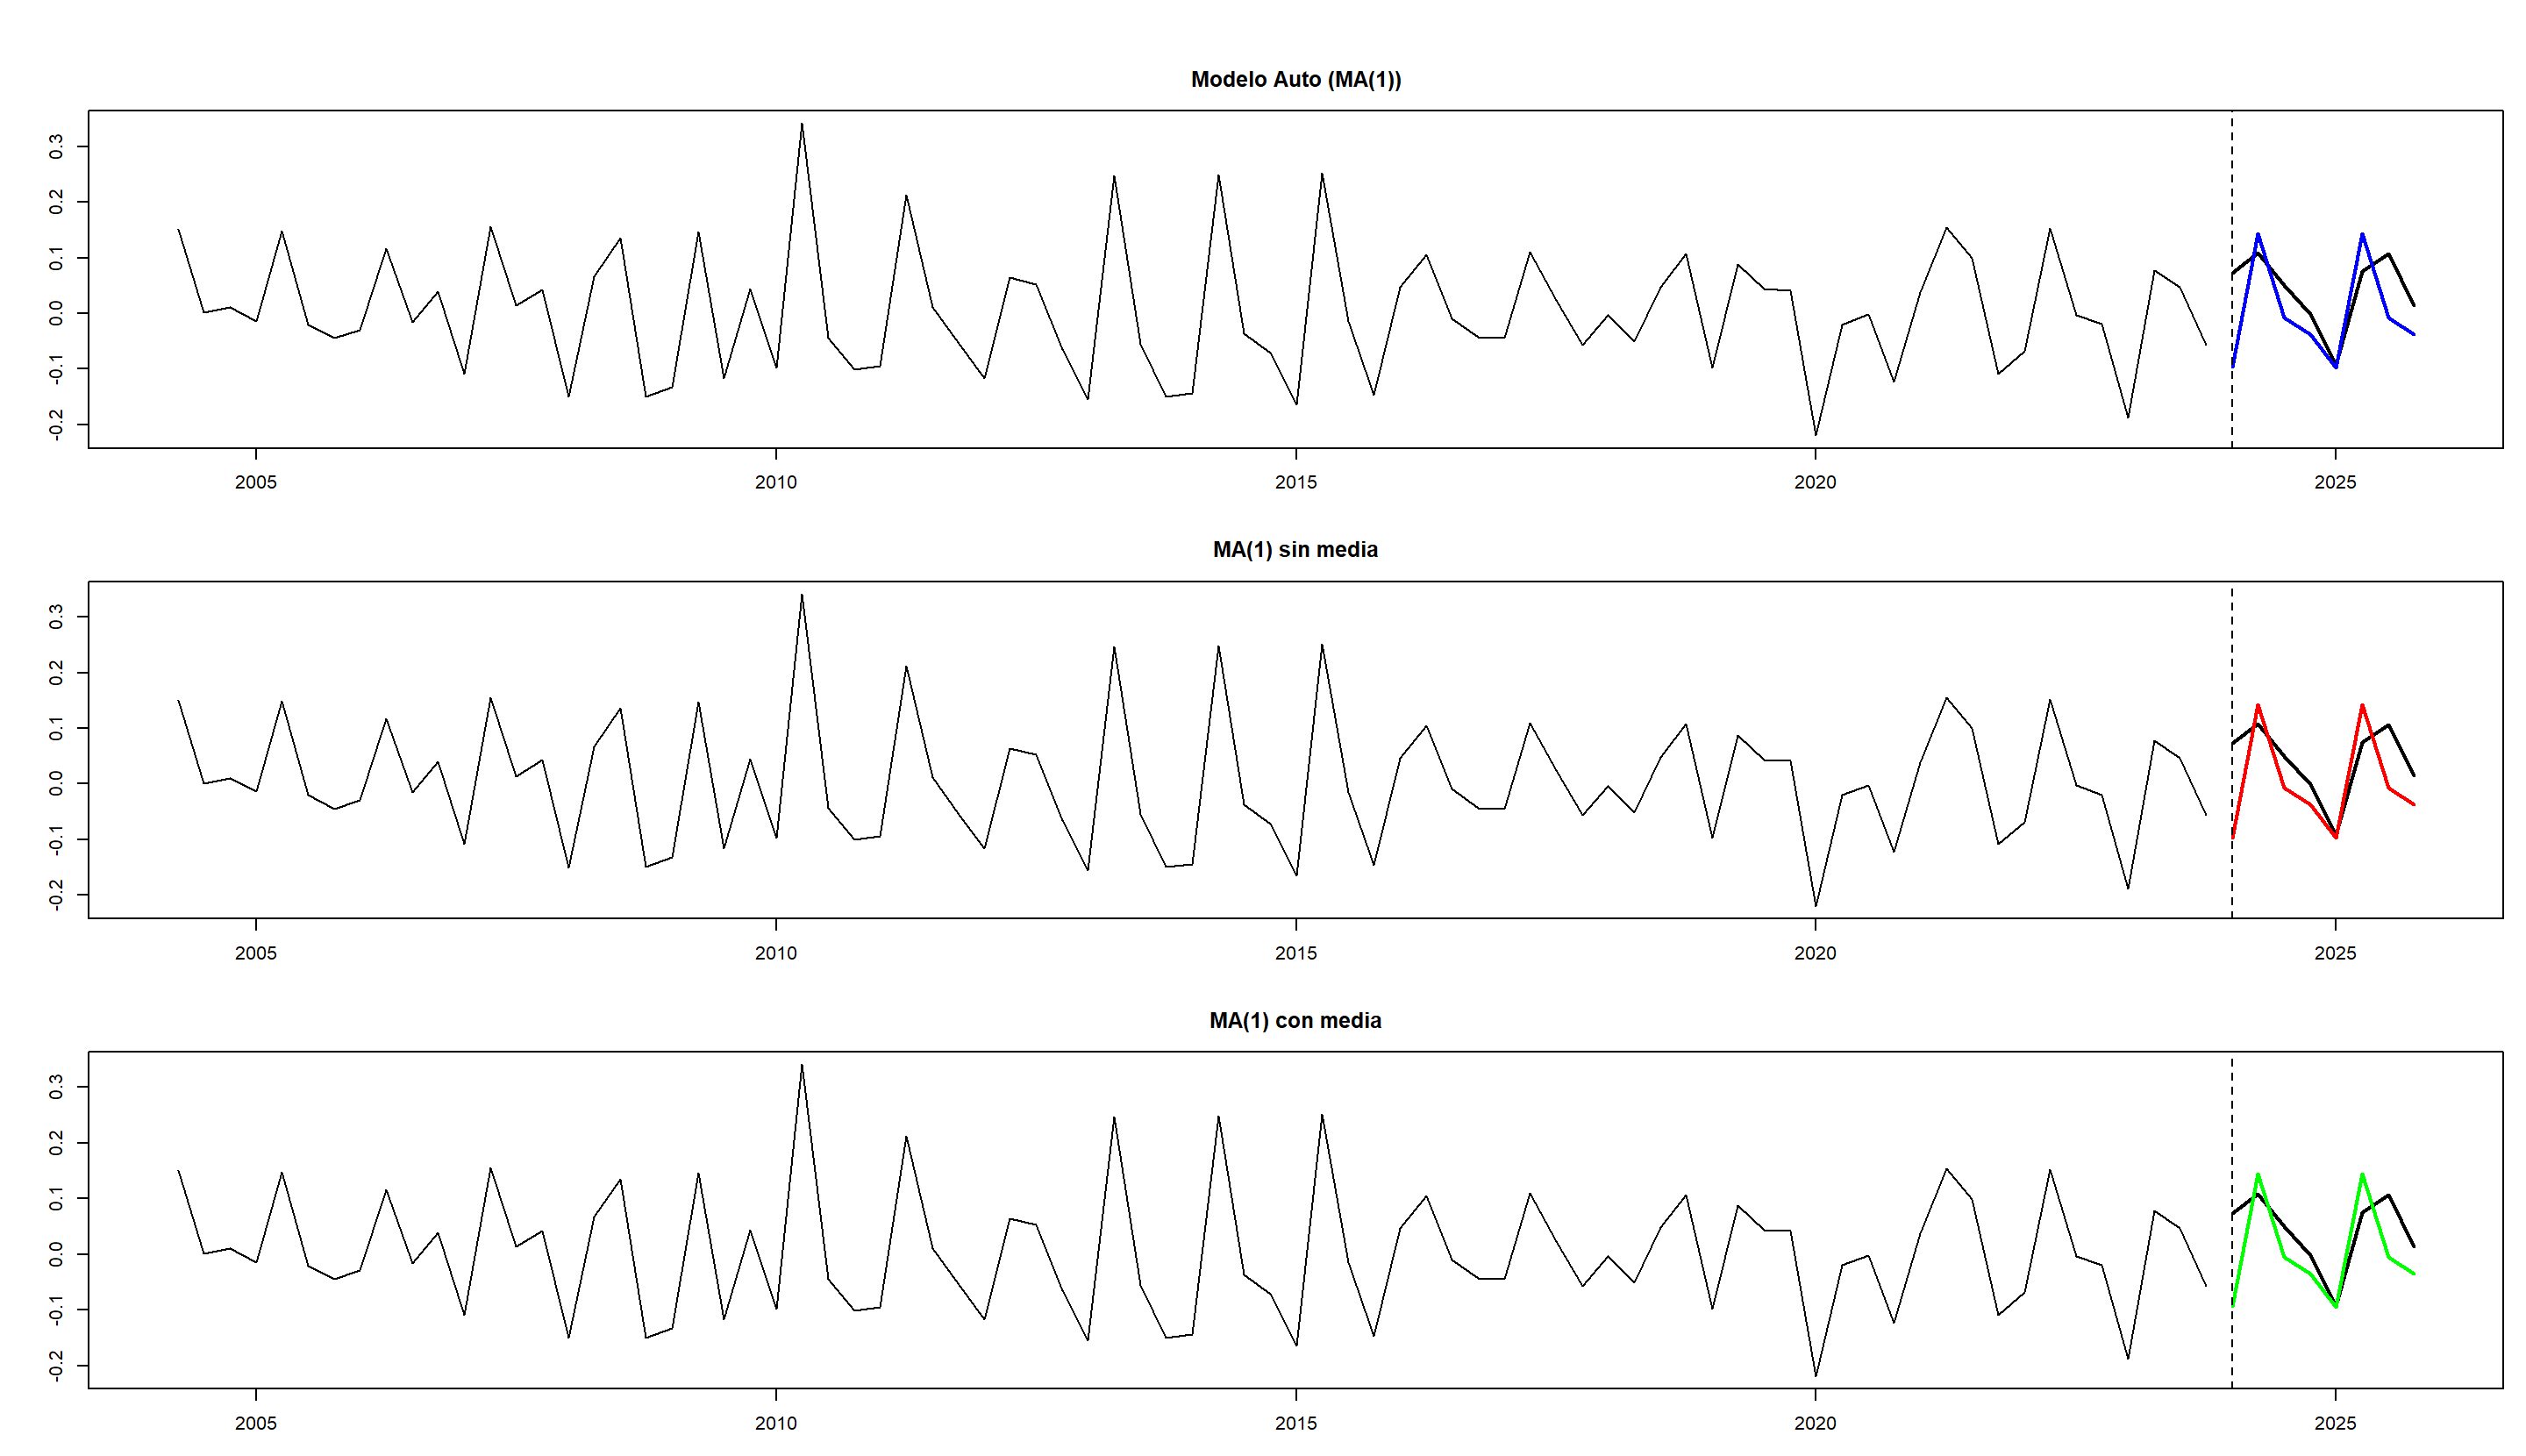
\includegraphics[width=0.95\textwidth]{14.png}
\caption{Comparación de pronósticos para la serie DL\_EXPO utilizando modelos MA(1) estimados sobre la serie desestacionalizada. La línea negra corresponde a la serie original observada (entrenamiento y valores reales), las líneas de color a los pronósticos y la línea vertical punteada indica el inicio del período de predicción.}
\label{fig:forecast_expo_ma1}
\end{figure}

El Cuadro~\ref{tab:forecast_expo} presenta la evaluación cuantitativa de estos pronósticos para el período 2024--2025. Los resultados muestran que el modelo automático y la especificación MA(1) sin media vuelven a ser exactamente equivalentes en todas las métricas, lo que refuerza la conclusión de que ambos representan, en esencia, la misma estructura estadística. Por su parte, el modelo MA(1) con media obtiene los menores valores de RMSE, MAE, MAPE y U de Theil, aunque la mejora es moderada en términos absolutos. Esto sugiere que incorporar una media distinta de cero aporta una pequeña ganancia predictiva una vez removida la estacionalidad, posiblemente porque permite recoger mejor un leve desplazamiento en el nivel medio de la dinámica ajustada. De todos modos, el desempeño de los modelos sobre la serie desestacionalizada sigue siendo inferior al observado para las mejores especificaciones SARIMA sobre la serie original, por lo que la desestacionalización no parece generar en este caso una ventaja clara en términos de capacidad predictiva global.

\begin{table}[H]
\centering
\caption{Evaluación de pronósticos – DL\_EXPO}
\label{tab:forecast_expo}
\begin{tabular}{lccc}
\hline
Métrica & Auto & MA(1) & MA(1) con media \\
\hline
RMSE    & 0.08283 & 0.08283 & 0.08135 \\
MAE     & 0.06704 & 0.06704 & 0.06566 \\
MAPE    & 475.46  & 475.46  & 447.19 \\
U de Theil & 0.50580 & 0.50580 & 0.49705 \\
\hline
\end{tabular}
\end{table}

El Cuadro~\ref{tab:global_expo} sintetiza la comparación global entre las estrategias de modelización aplicadas a DL\_EXPO. La evidencia muestra que los modelos SARIMA estimados sobre la serie original dominan a las alternativas basadas en la serie desestacionalizada en las métricas más robustas de desempeño predictivo, particularmente RMSE, MAE y U de Theil. En efecto, tanto el modelo SARIMA automático como la especificación SARIMA MA superan a todas las variantes estimadas sobre la serie ajustada, mientras que el SARIMA AR(2) también resulta competitivo, aunque algo menos favorable que las dos opciones más parsimoniosas. Es cierto que los modelos desestacionalizados exhiben valores menores de MAPE, especialmente en la variante MA(1) con media; sin embargo, dado que la serie está expresada en diferencias logarítmicas y toma valores cercanos a cero, esa métrica debe interpretarse con cautela. Por ello, al ponderar conjuntamente el error cuadrático, el error absoluto y el coeficiente U de Theil, la conclusión general favorece la modelización directa de la estacionalidad mediante especificaciones SARIMA.

\begin{table}[H]
\centering
\caption{Comparación global de modelos de pronóstico – DL\_EXPO}
\label{tab:global_expo}
\resizebox{\textwidth}{!}{%
\begin{tabular}{lcccccc}
\hline
Métrica & SARIMA Auto & SARIMA MA & SARIMA AR & SA Auto & SA MA(1) & SA MA(1) media \\
\hline
RMSE    & 0.06972 & 0.06972 & 0.07794 & 0.08283 & 0.08283 & 0.08135 \\
MAE     & 0.05436 & 0.05436 & 0.06084 & 0.06704 & 0.06704 & 0.06566 \\
MAPE    & 551.50  & 551.50  & 571.31  & 475.46  & 475.46  & 447.19 \\
U de Theil & 0.45292 & 0.45292 & 0.48760 & 0.50580 & 0.50580 & 0.49705 \\
\hline
\end{tabular}%
}
\end{table}

En síntesis, el análisis de la serie de exportaciones indica que la eliminación previa de la estacionalidad no genera una mejora suficiente como para desplazar a los modelos SARIMA estimados sobre la serie original. Si bien la desestacionalización simplifica la estructura temporal y permite trabajar con especificaciones ARMA muy parsimoniosas, esa simplificación no se traduce en una mayor precisión predictiva fuera de muestra. Por lo tanto, para DL\_EXPO la evidencia empírica sugiere que resulta preferible conservar la información estacional dentro del modelo y tratarla de manera explícita. A continuación, se desarrolla el mismo ejercicio para la inversión bruta fija, una variable que suele exhibir una volatilidad todavía mayor y cuya dinámica puede ofrecer un contraste interesante respecto de los casos anteriores.

\subsection{Inversión bruta fija (DL\_IBF)}

La Figura~\ref{fig:dl_ibf} presenta la evolución de la serie DL\_IBF en diferencias logarítmicas para el período analizado. A diferencia de variables más estables, la inversión bruta fija exhibe oscilaciones de mayor amplitud alrededor de cero, con alternancia frecuente entre tasas de crecimiento positivas y negativas y con episodios de volatilidad particularmente intensa. Este comportamiento es consistente con la naturaleza procíclica de la inversión y su elevada sensibilidad frente a shocks macroeconómicos, por lo que, si bien la transformación en diferencias logarítmicas aproxima la serie a la estacionariedad en media, la dinámica remanente sigue siendo relativamente errática y exige un examen cuidadoso de su estructura temporal.

\begin{figure}[H]
\centering
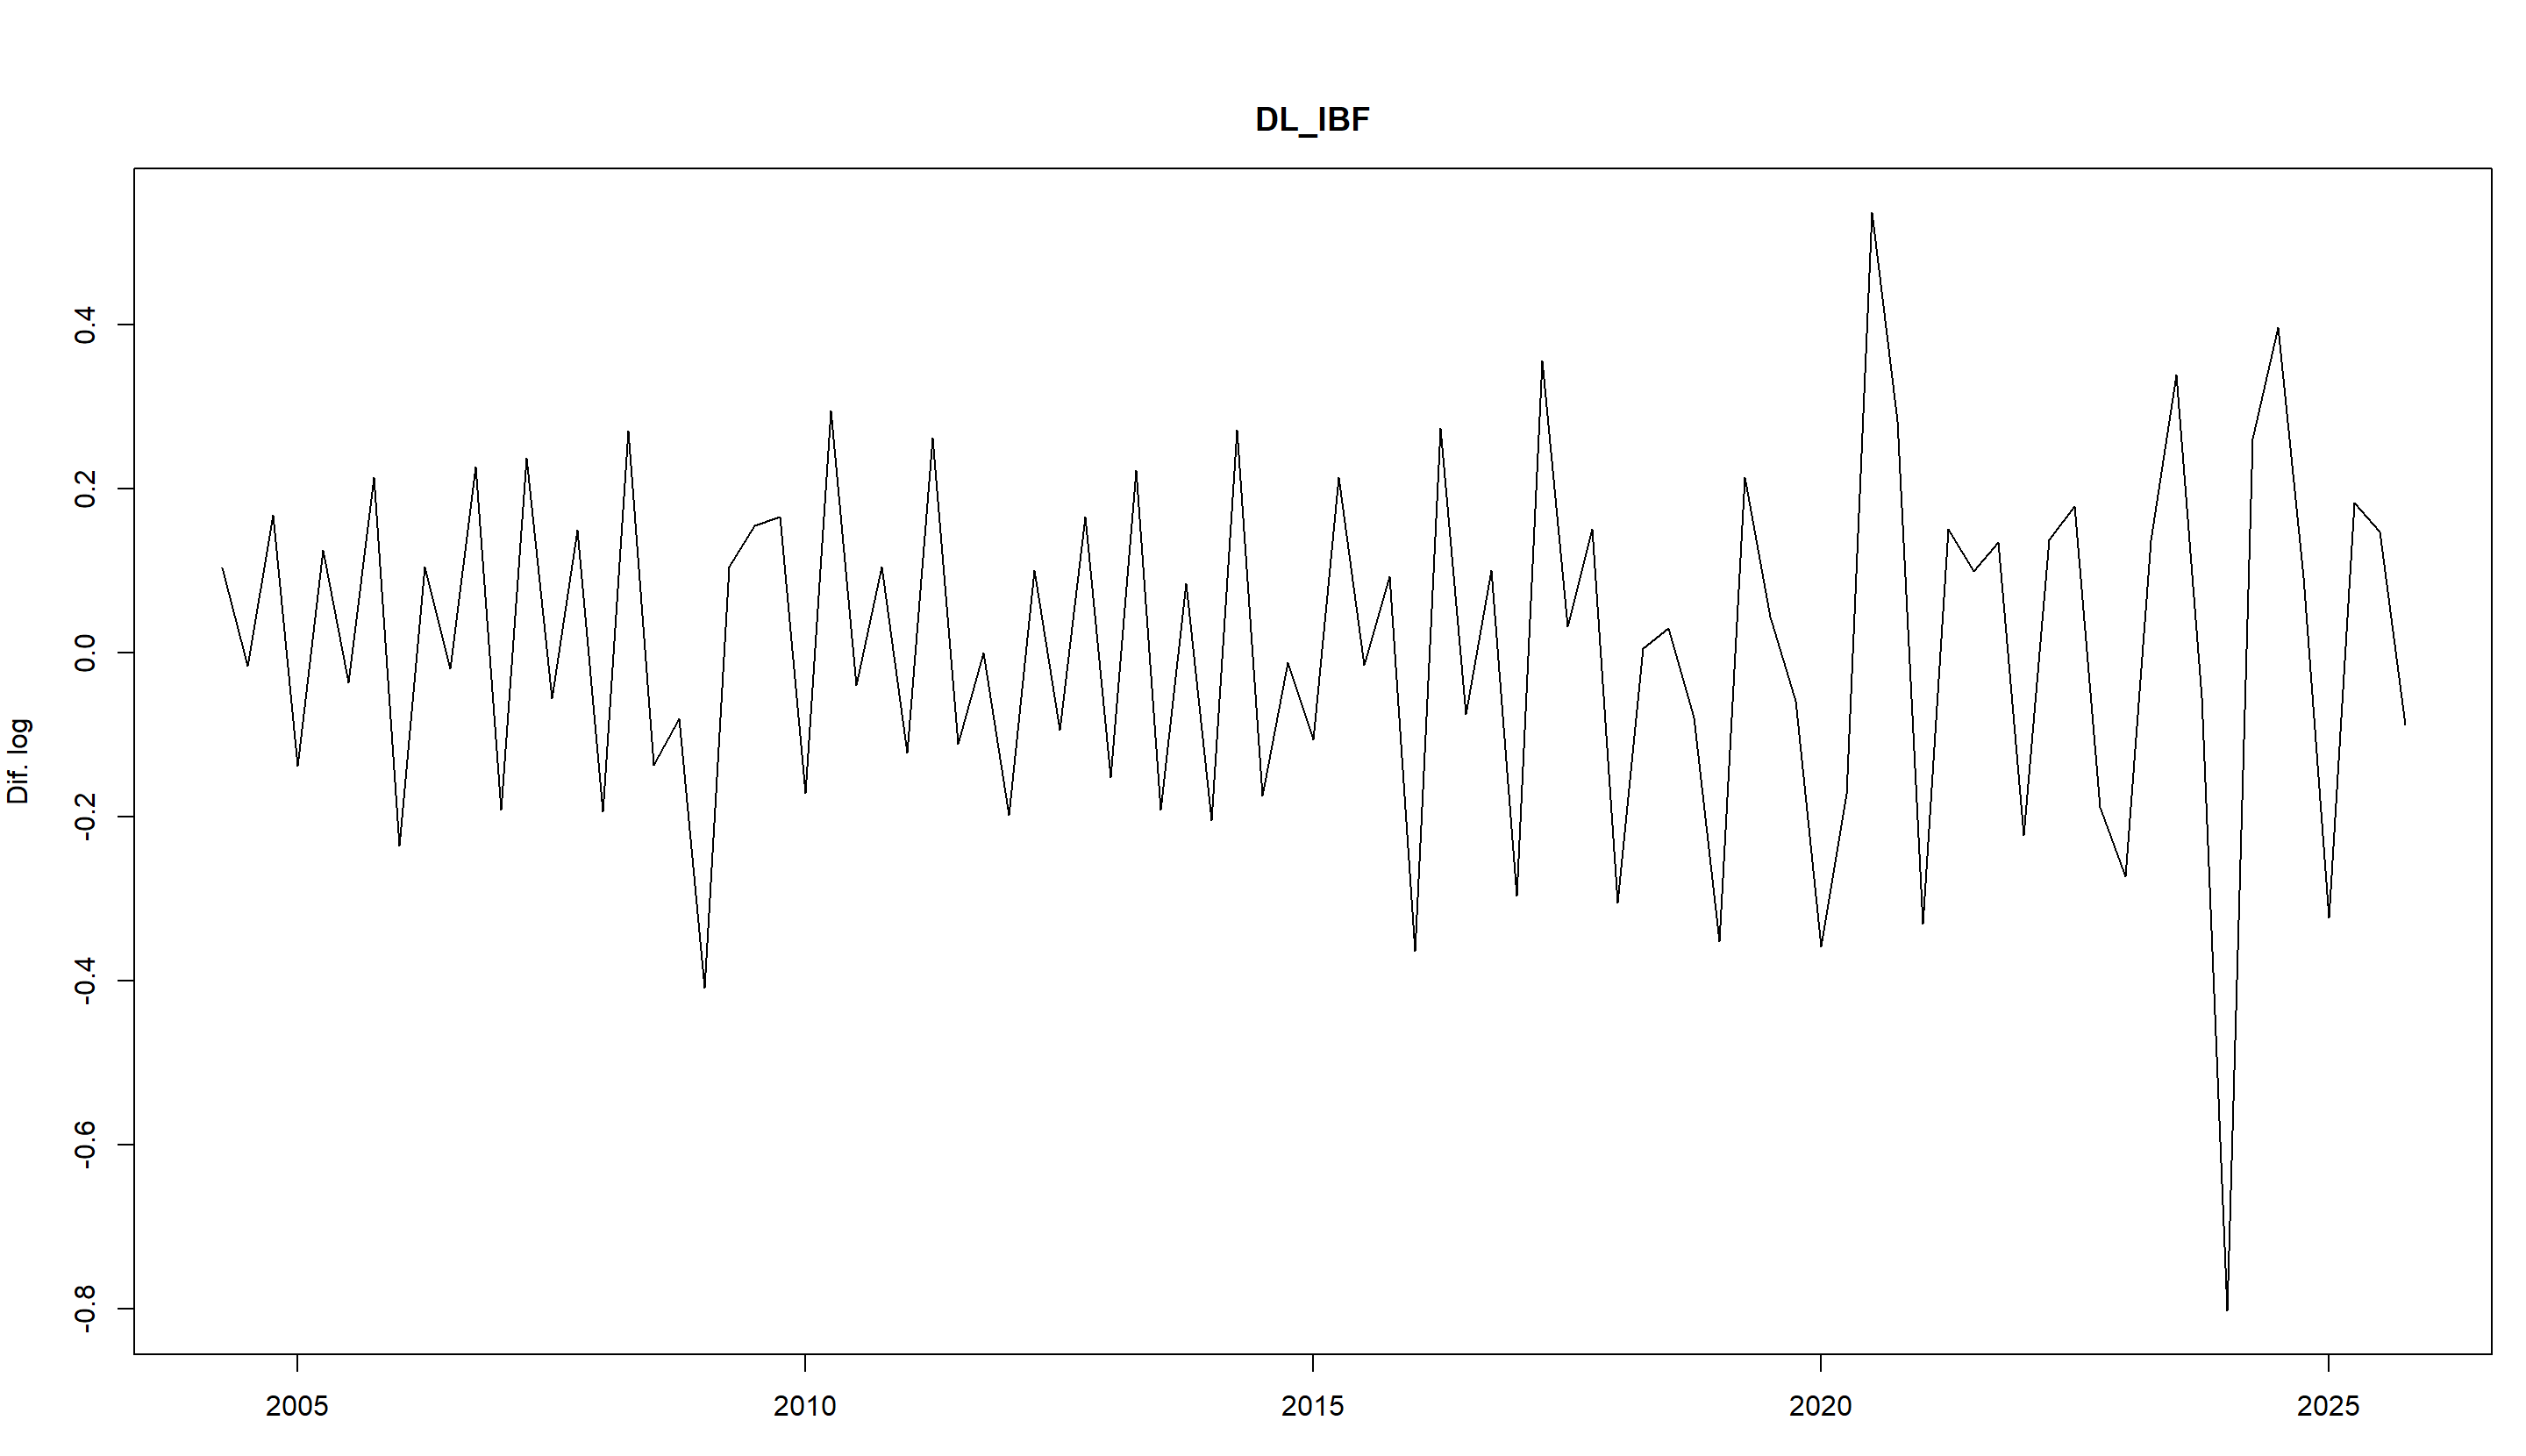
\includegraphics[width=0.95\textwidth]{15.png}
\caption{Serie DL\_IBF, correspondiente a las diferencias logarítmicas de la Inversión Bruta Fija (aproximación a su tasa de crecimiento trimestral), para el período 2004–2025. La serie presenta fluctuaciones alrededor de cero, consistentes con un comportamiento estacionario, aunque con episodios de mayor volatilidad, particularmente en períodos recientes.}
\label{fig:dl_ibf}
\end{figure}

Las Figuras~\ref{fig:acf_ibf} y~\ref{fig:pacf_ibf} muestran los correlogramas ACF y PACF de DL\_IBF. En la ACF se observan autocorrelaciones relevantes en los primeros rezagos y señales compatibles con la presencia de un patrón estacional trimestral, lo que sugiere que la serie conserva cierta regularidad sistemática aun después de la transformación aplicada. Por su parte, la PACF concentra la significatividad en pocos rezagos iniciales y exhibe una estructura relativamente acotada, consistente con la consideración de modelos de bajo orden. En conjunto, la evidencia gráfica sugiere que la dinámica de la inversión bruta fija puede modelizarse mediante especificaciones parsimoniosas, aunque conviene permitir la incorporación de componentes estacionales y contrastar alternativas autorregresivas y de media móvil.

\begin{figure}[H]
\centering
\begin{subfigure}[t]{0.48\textwidth}
\centering
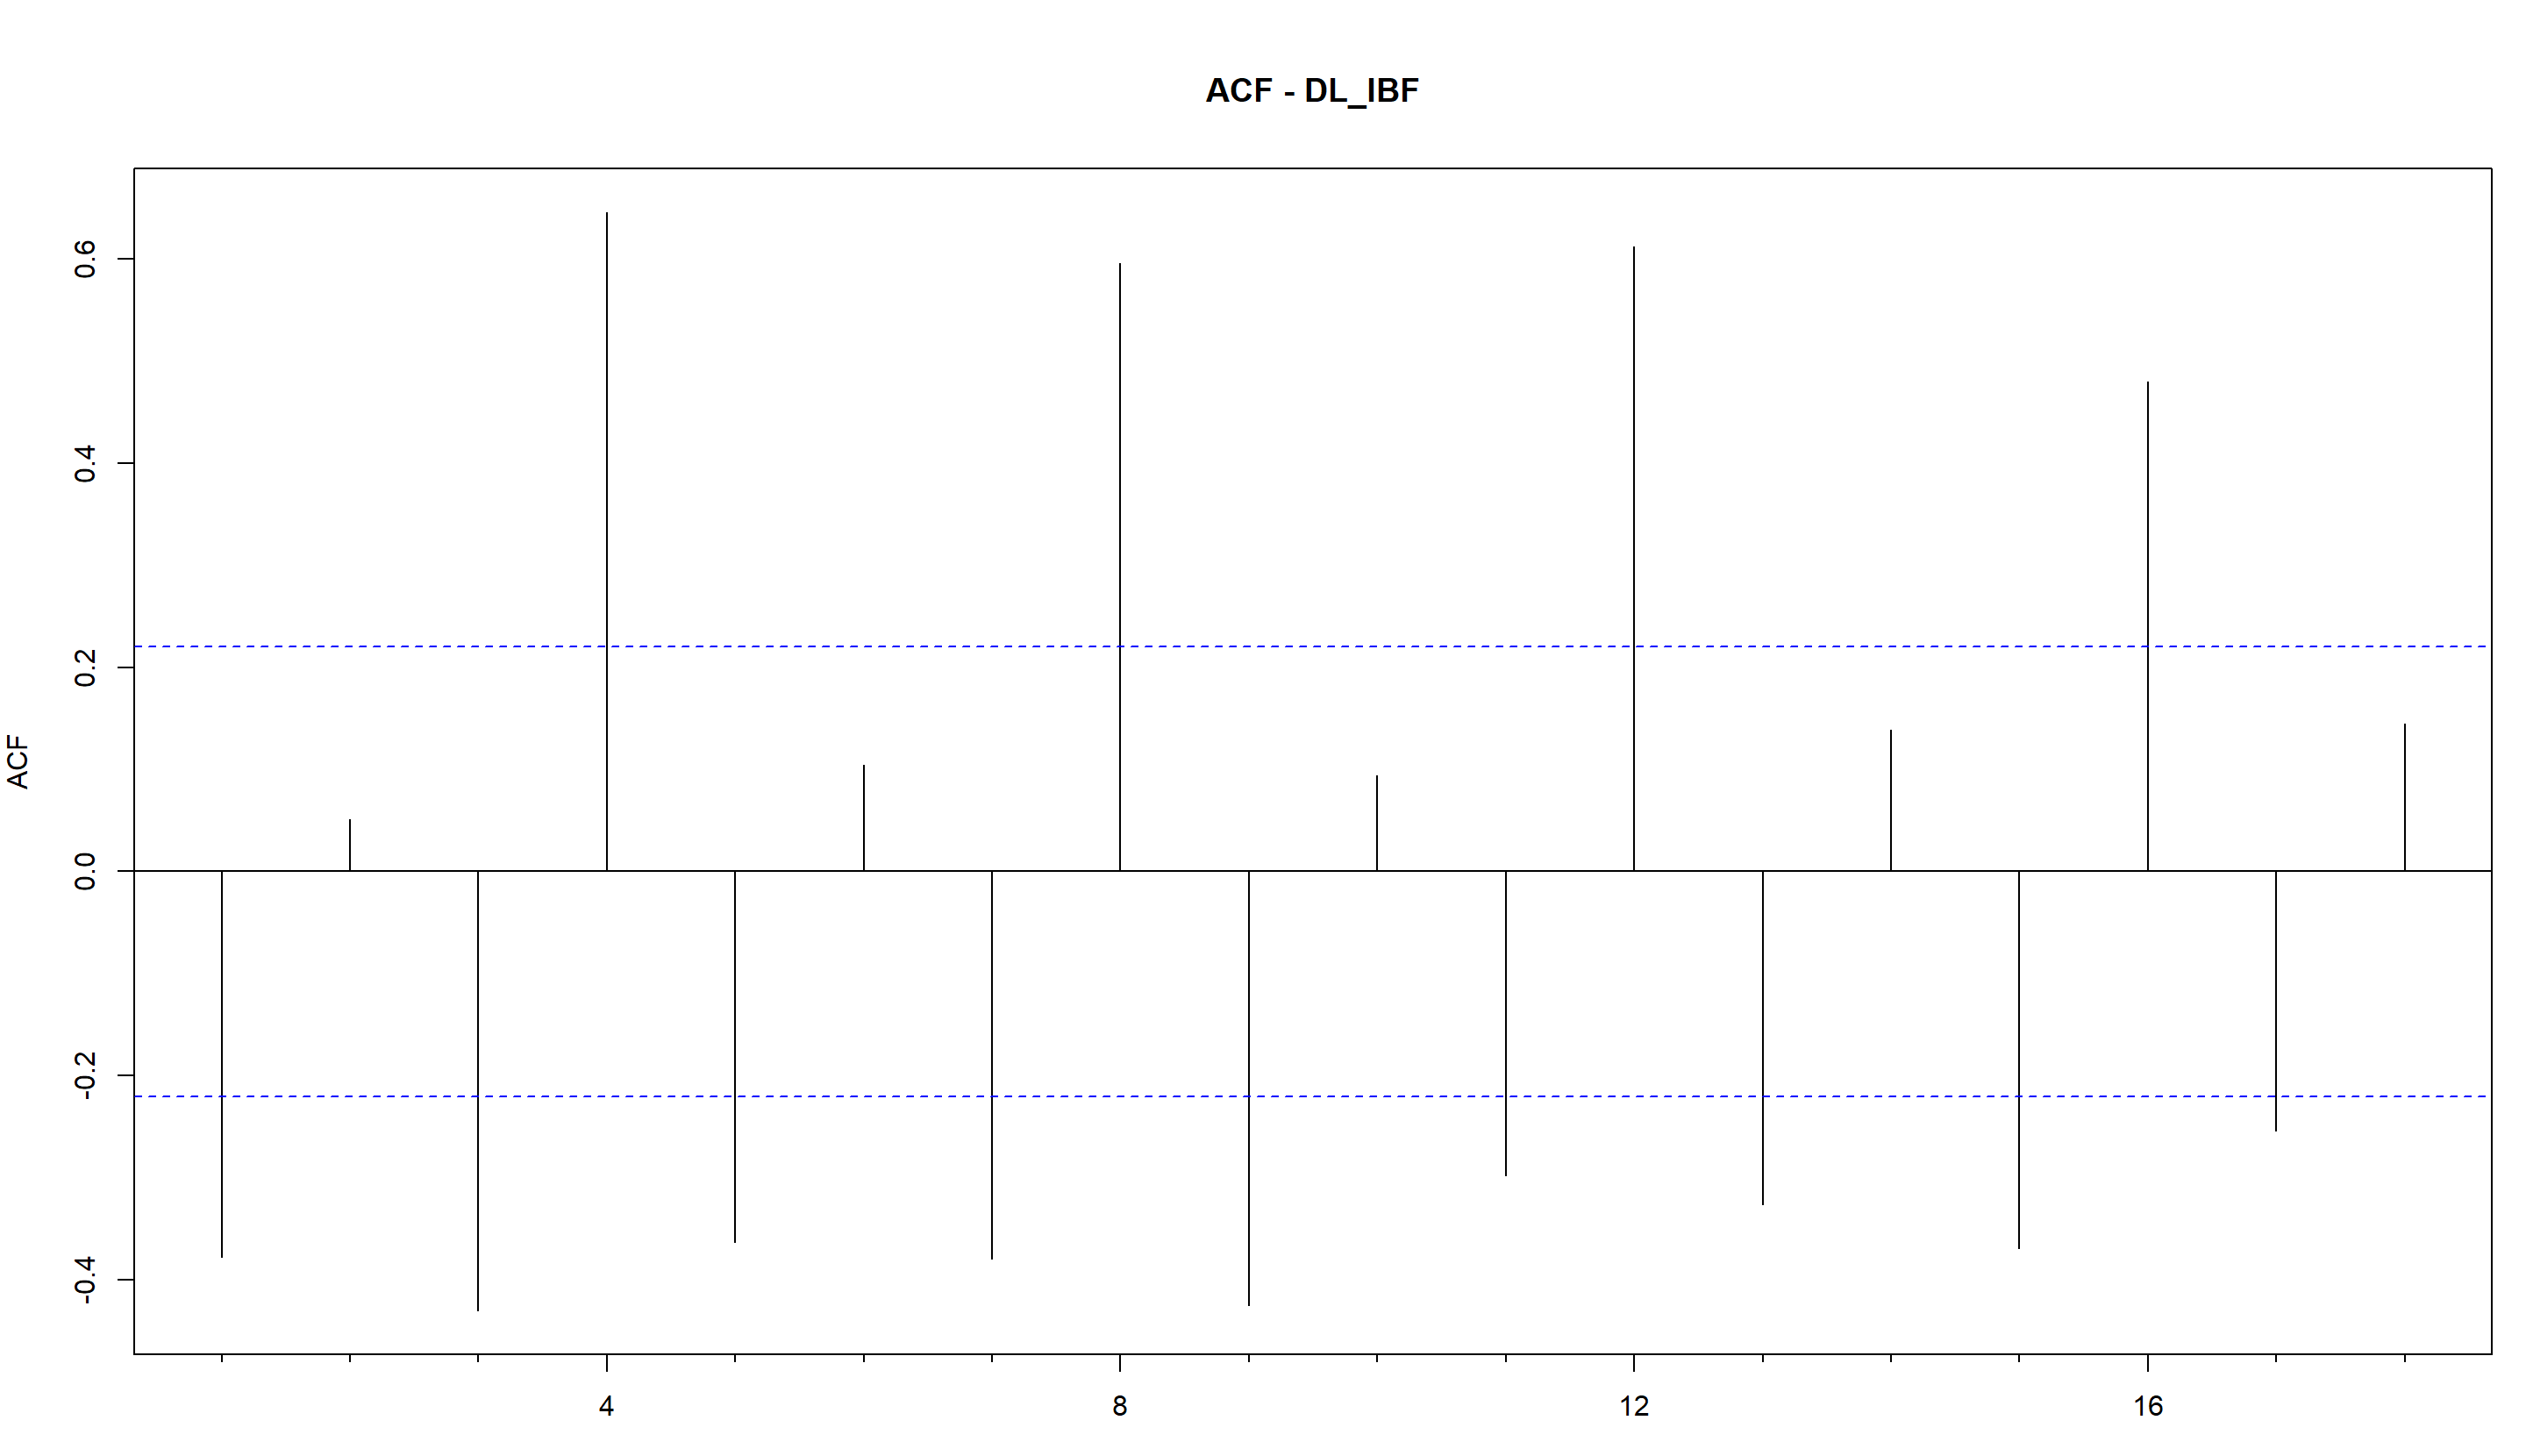
\includegraphics[width=\textwidth]{16.png}
\caption{Función de autocorrelación (ACF) de la serie DL\_IBF.}
\label{fig:acf_ibf}
\end{subfigure}
\hfill
\begin{subfigure}[t]{0.48\textwidth}
\centering
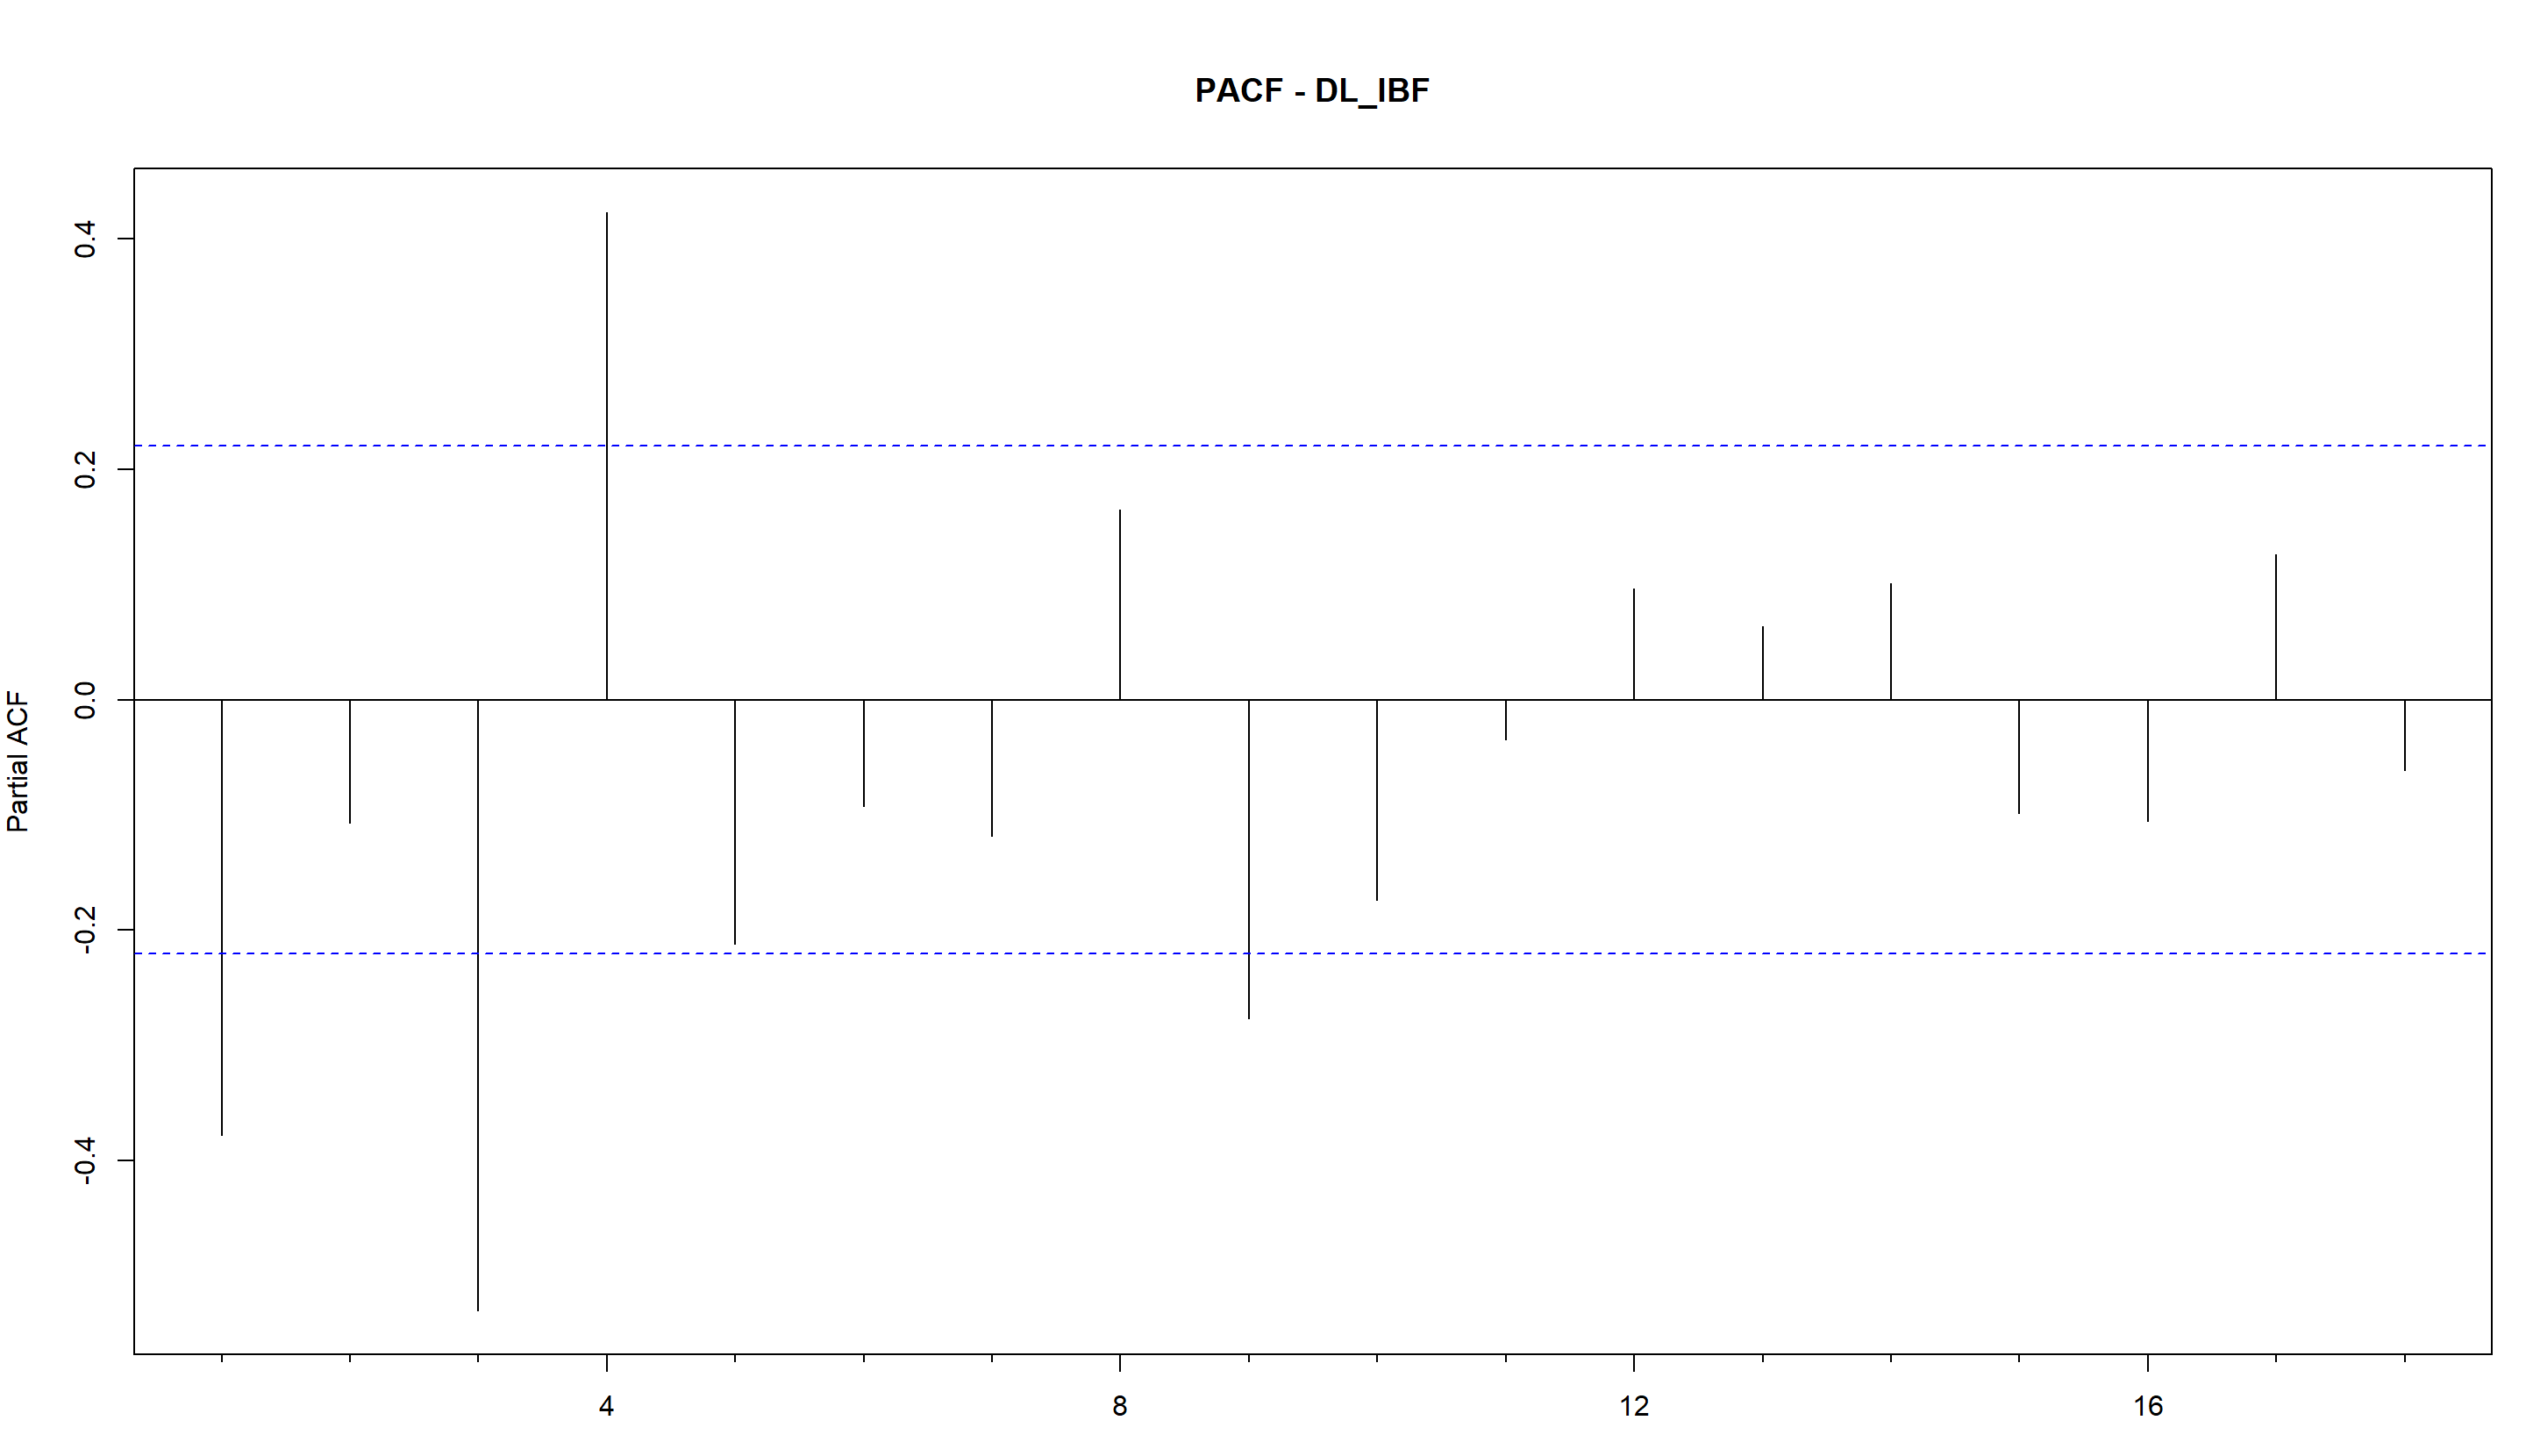
\includegraphics[width=\textwidth]{17.png}
\caption{Función de autocorrelación parcial (PACF) de la serie DL\_IBF.}
\label{fig:pacf_ibf}
\end{subfigure}
\end{figure}

El Cuadro~\ref{tab:sarima_ibf} resume la comparación entre las especificaciones SARIMA manuales consideradas para la serie DL\_IBF. Los resultados muestran que los modelos MA(1) y AR(1) presentan un desempeño dentro de la muestra prácticamente indistinguible, con diferencias mínimas en términos de AIC, RMSE, MAE y MASE. No obstante, la especificación MA(1) exhibe una leve ventaja global: presenta el menor AIC, errores apenas inferiores y una autocorrelación residual más cercana a cero, lo que sugiere una representación algo más parsimoniosa y equilibrada de la dinámica de la inversión. Al mismo tiempo, el MAPE alcanza valores muy elevados en ambas alternativas, por lo que debe interpretarse con cautela, dado que la serie está expresada en diferencias logarítmicas y toma valores próximos a cero, circunstancia que tiende a amplificar esta métrica relativa.

\begin{table}[H]
\centering
\caption{Comparación de modelos SARIMA – DL\_IBF}
\label{tab:sarima_ibf}
\begin{tabular}{lcccccc}
\hline
Modelo & AIC & RMSE & MAE & MAPE & MASE & ACF (res.) \\
\hline
SARIMA MA(1) & -85.21 & 0.1263044 & 0.08716487 & 942.4004 & 0.7479492 & -0.005599421 \\
SARIMA AR(1) & -85.18 & 0.1263123 & 0.08720398 & 951.4972 & 0.7482848 & 0.003164345 \\
\hline
\end{tabular}
\end{table}

El Cuadro~\ref{tab:diag_ibf} presenta los diagnósticos residuales de las especificaciones consideradas para DL\_IBF. En los tres casos, los p-valores de las pruebas de Ljung-Box y Box-Ljung se ubican por encima de los niveles usuales de significatividad, de modo que no se rechaza la hipótesis nula de ausencia de autocorrelación serial en los residuos. Esto indica que tanto el modelo automático como las alternativas manuales resultan estadísticamente admisibles desde el punto de vista del diagnóstico. Si bien las diferencias entre p-valores son pequeñas y no alteran la conclusión general, el modelo automático muestra una ligera ventaja en la prueba de Ljung-Box, mientras que la especificación MA(1) aparece marginalmente mejor posicionada en Box-Ljung. En conjunto, la evidencia diagnóstica confirma que las tres alternativas limpian razonablemente bien la dependencia serial de la serie y habilitan la comparación de su desempeño predictivo fuera de muestra.

\begin{table}[H]
\centering
\caption{Diagnóstico de residuos – DL\_IBF}
\label{tab:diag_ibf}
\begin{tabular}{lcc}
\hline
Modelo & Ljung-Box (p-valor) & Box-Ljung (p-valor) \\
\hline
SARIMA automático & 0.3559 & 0.2041 \\
SARIMA MA(1)      & 0.3011 & 0.2513 \\
SARIMA AR(1)      & 0.2890 & 0.2381 \\
\hline
\end{tabular}
\end{table}

La Figura~\ref{fig:forecast_ibf_models} compara los pronósticos fuera de muestra generados por las tres especificaciones SARIMA consideradas para DL\_IBF. Visualmente, las trayectorias pronosticadas son muy similares entre sí y reproducen una dinámica oscilante alrededor de cero, lo que sugiere que los tres modelos capturan de manera parecida la evolución esperada de corto plazo de la inversión bruta fija. Aun así, se advierte que la serie observada presenta movimientos relativamente bruscos y cambios de amplitud que resultan difíciles de anticipar con precisión, de modo que las diferencias entre especificaciones son necesariamente sutiles. En ese contexto, el modelo MA(1) y la variante automática exhiben trayectorias prácticamente superpuestas y bandas de confianza muy cercanas, mientras que el AR(1) tampoco se aparta de forma sustantiva del patrón general, lo que refuerza la idea de que la ganancia potencial de complejizar la estructura dinámica es acotada en esta serie.

\begin{figure}[H]
\centering
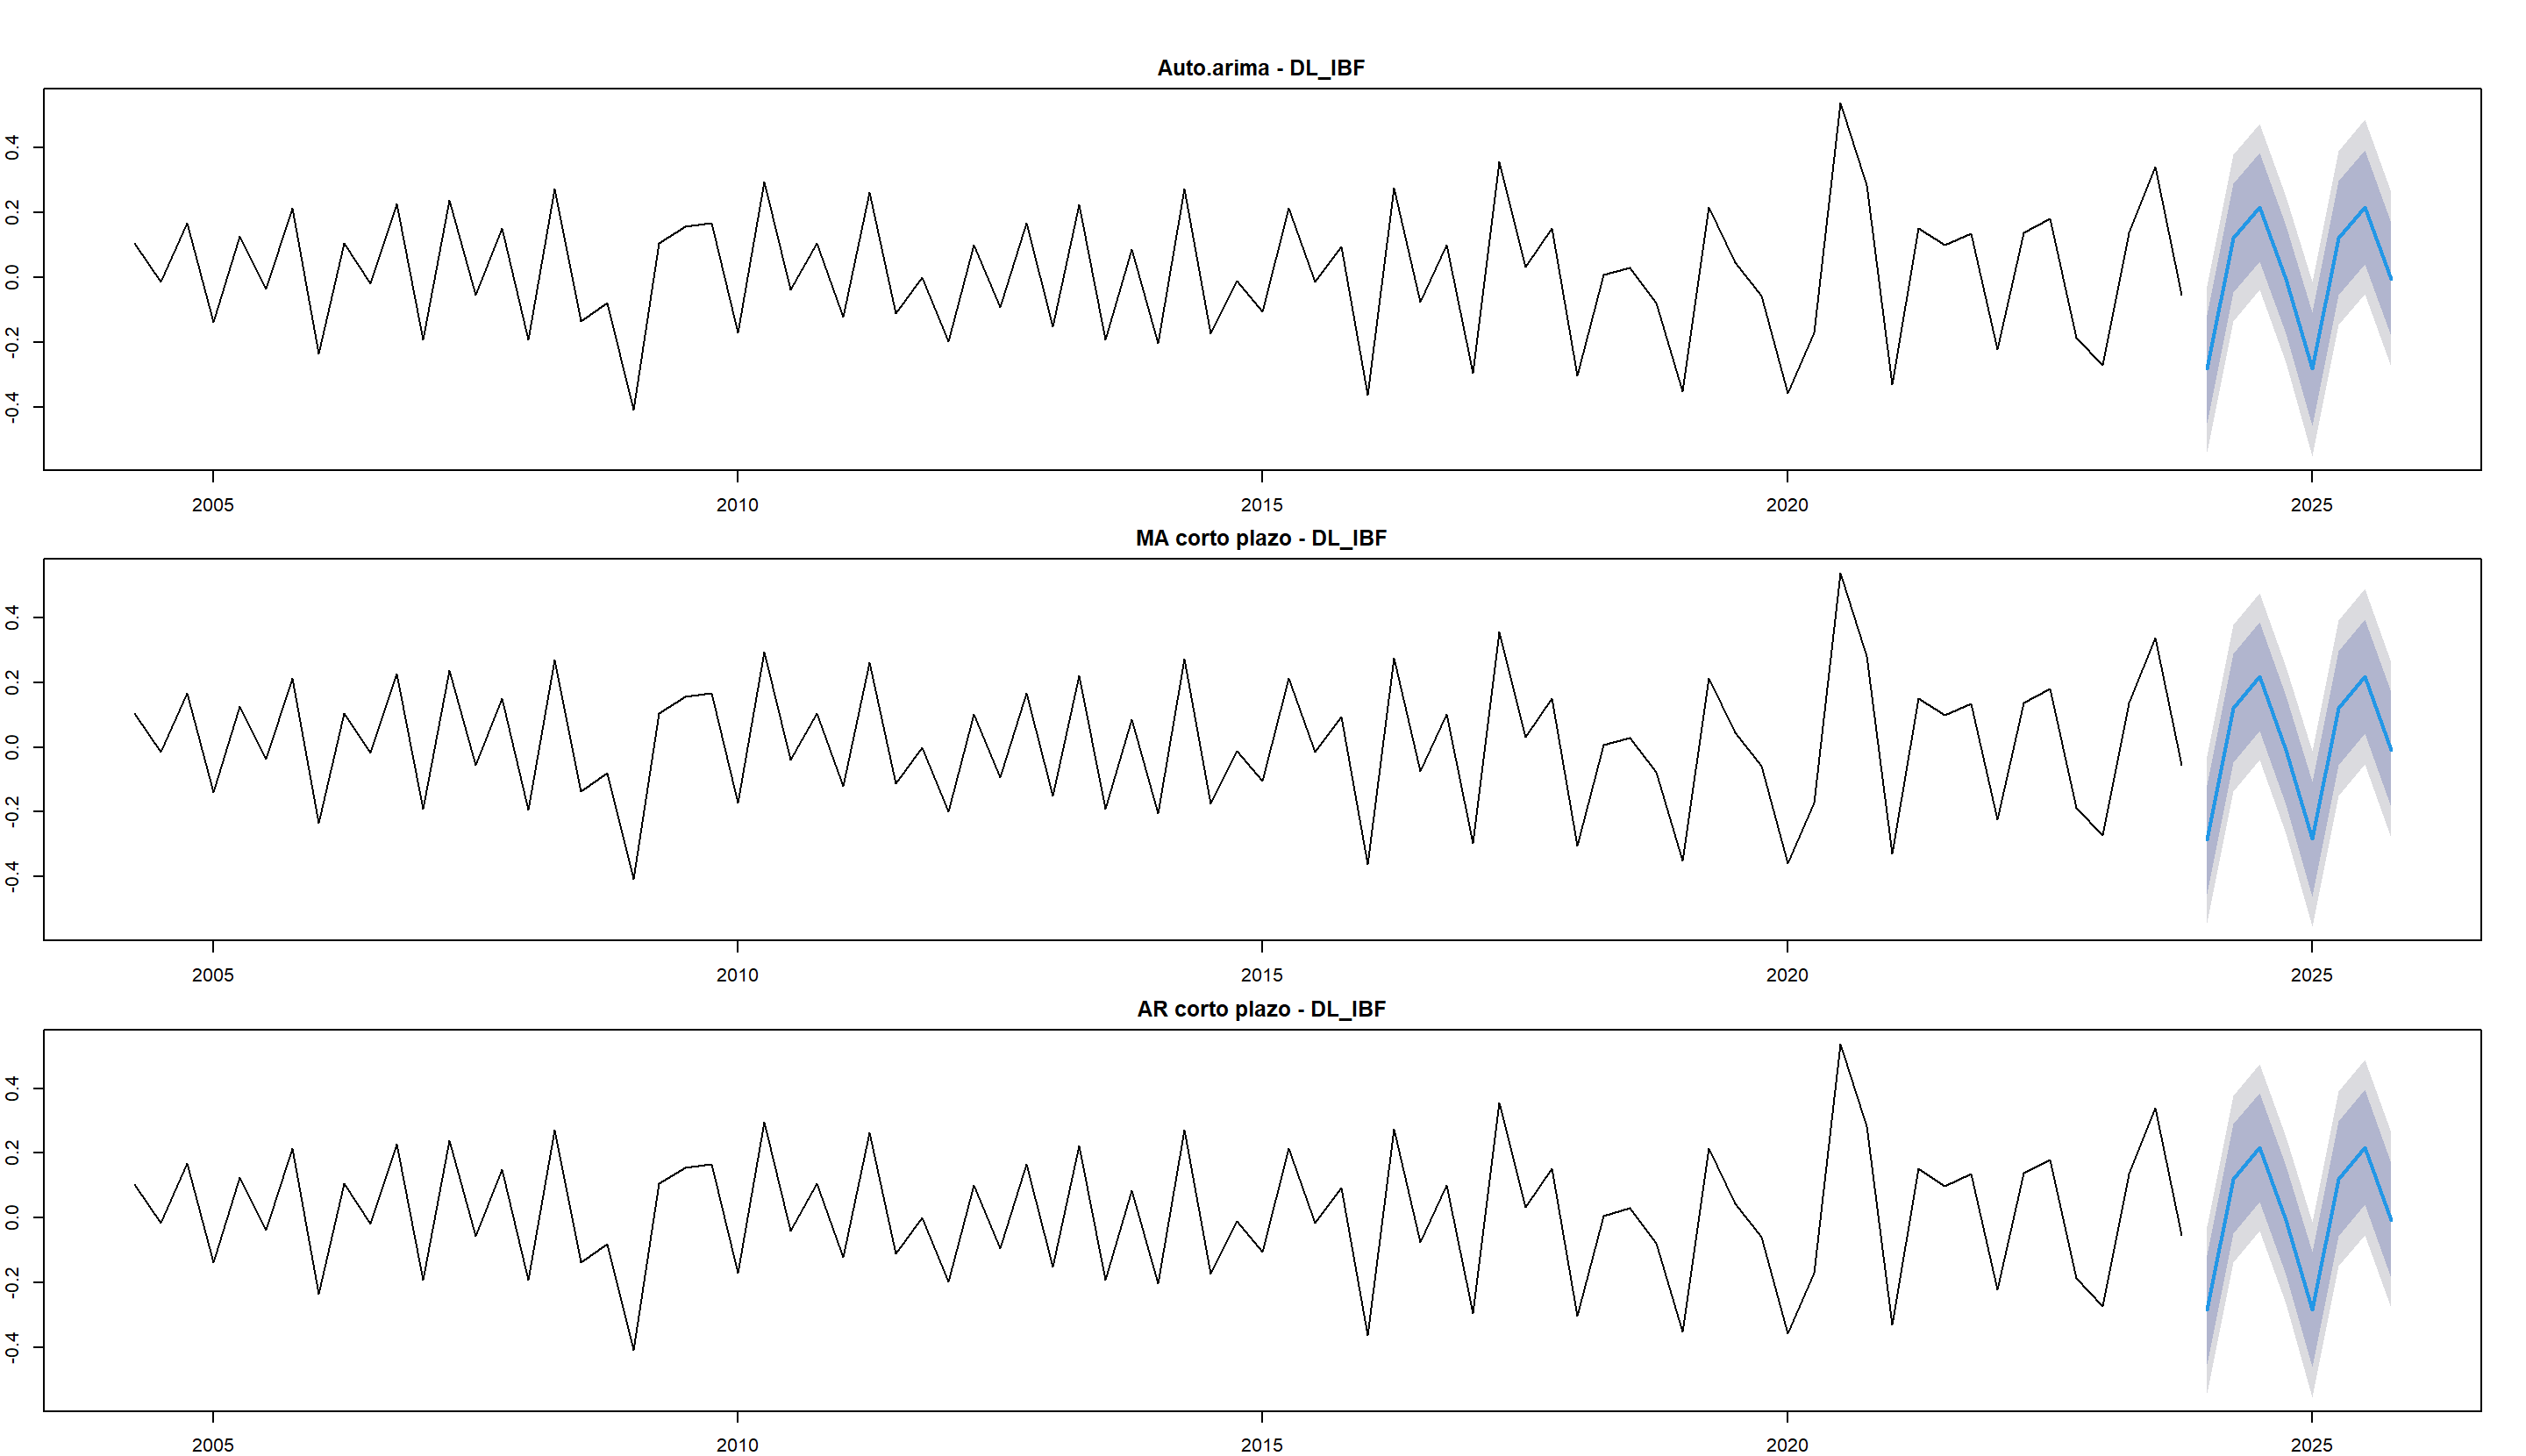
\includegraphics[width=0.95\textwidth]{18.png}
\caption{Comparación de pronósticos para la serie DL\_IBF (diferencias logarítmicas de la Inversión Bruta Fija) utilizando tres especificaciones: modelo automático, MA(1) y AR(1). La línea negra corresponde a la serie observada, las líneas de color a los pronósticos y las bandas sombreadas representan los intervalos de confianza.}
\label{fig:forecast_ibf_models}
\end{figure}

El Cuadro~\ref{tab:forecast_ibf} presenta la evaluación cuantitativa del desempeño predictivo fuera de muestra para el período 2024--2025. Los resultados indican que las tres especificaciones ofrecen un rendimiento muy parecido, aunque el modelo SARIMA MA(1) obtiene los mejores valores de RMSE, MAE y U de Theil, lo que lo ubica levemente por encima de sus competidores cuando se priorizan las métricas más robustas. El modelo AR(1) también se mantiene muy próximo al MA(1), mientras que la especificación automática muestra errores apenas mayores, aunque la diferencia es reducida en términos absolutos. En cambio, el MAPE vuelve a presentar escasa capacidad discriminante, ya que sus valores son muy similares y, además, deben interpretarse con cautela por tratarse de una serie en diferencias logarítmicas con observaciones cercanas a cero. En consecuencia, la evidencia fuera de muestra favorece marginalmente al modelo MA(1), aunque la proximidad entre los resultados sugiere que la capacidad predictiva de las tres alternativas es, en términos prácticos, bastante semejante.

\begin{table}[H]
\centering
\caption{Evaluación de desempeño predictivo (fuera de muestra) – DL\_IBF}
\label{tab:forecast_ibf}
\begin{tabular}{lcccc}
\hline
Modelo & RMSE & MAE & MAPE & U de Theil \\
\hline
SARIMA automático & 0.20864800 & 0.14895409 & 57.04265516 & 0.37951075 \\
SARIMA MA(1)      & 0.20763579 & 0.14855479 & 57.10475761 & 0.37676572 \\
SARIMA AR(1)      & 0.20796530 & 0.14870410 & 57.10214770 & 0.37762780 \\
\hline
\end{tabular}
\end{table}

La Figura~\ref{fig:dl_ibf_sa} presenta la serie DL\_IBF una vez removido el componente estacional mediante el procedimiento X-13. En comparación con la serie original, la trayectoria desestacionalizada conserva la elevada volatilidad característica de la inversión bruta fija, pero exhibe oscilaciones algo más depuradas del patrón trimestral regular. La serie sigue fluctuando alrededor de cero y mantiene episodios de cambios bruscos, lo que sugiere que la desestacionalización elimina parte de la periodicidad sistemática, aunque no modifica el carácter marcadamente sensible de la inversión frente a shocks transitorios y variaciones del ciclo económico. En este sentido, la versión ajustada ofrece una base útil para evaluar si una especificación no estacional más simple resulta suficiente para describir la dinámica remanente.

\begin{figure}[H]
\centering
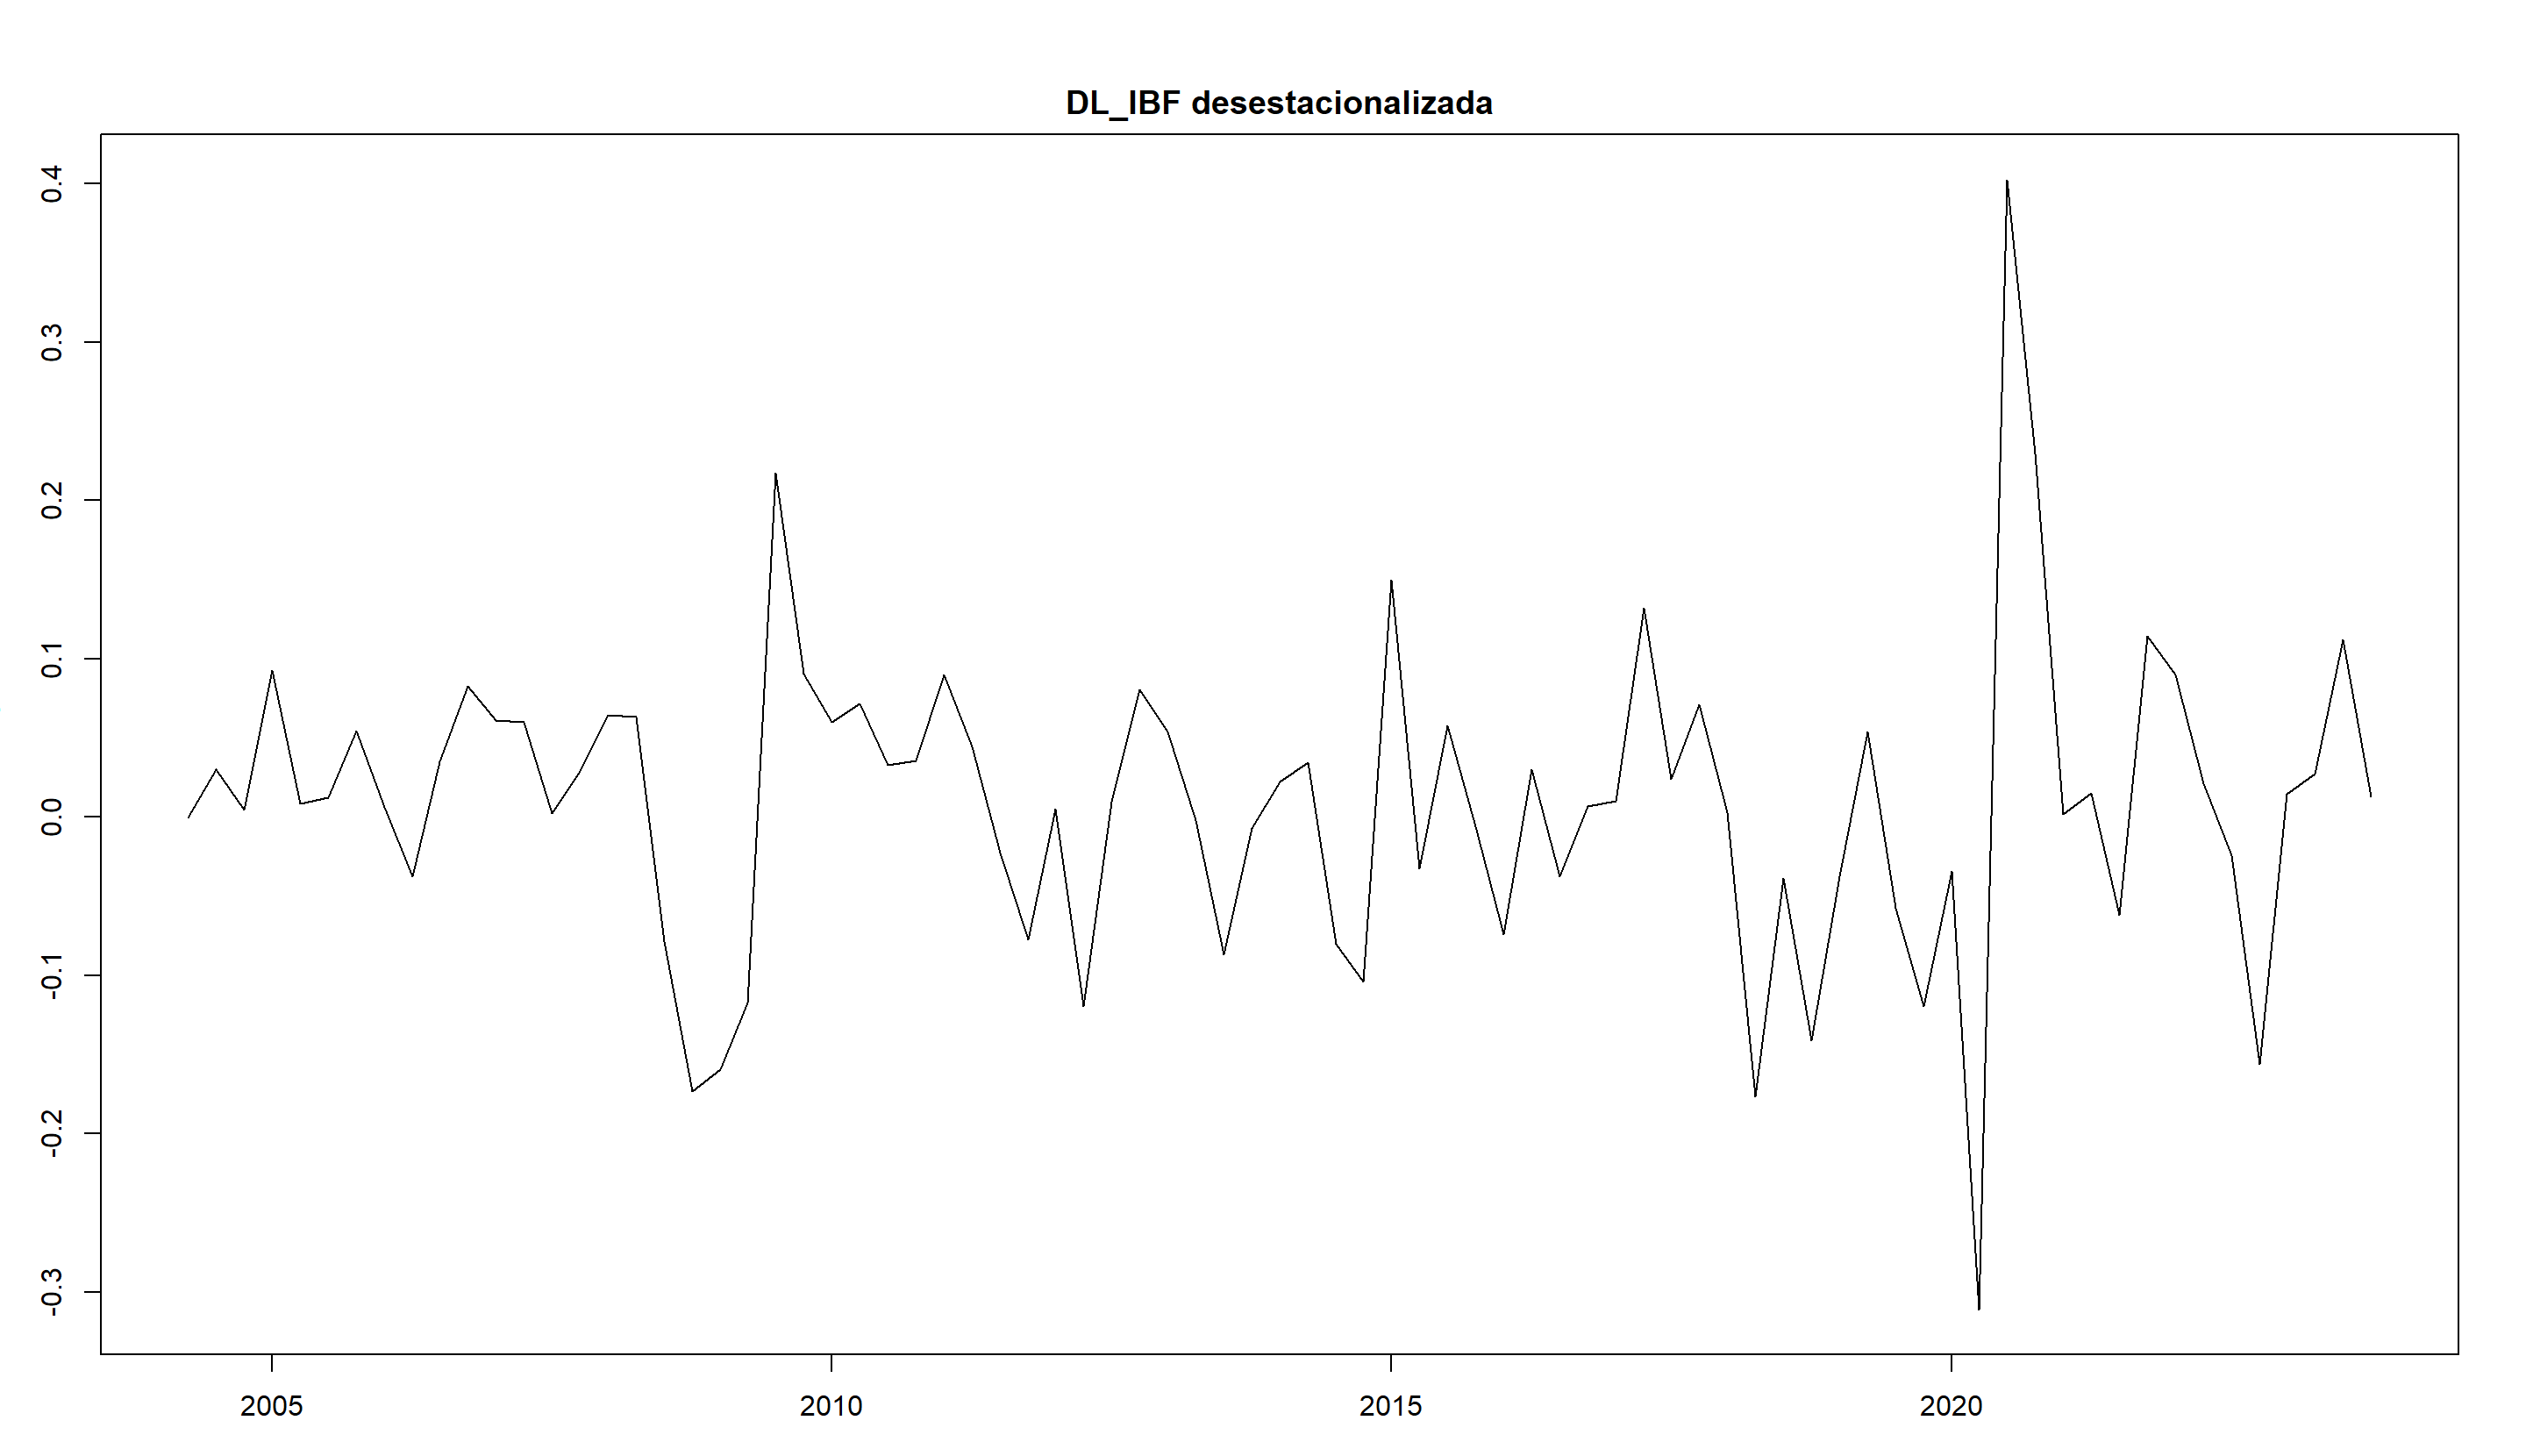
\includegraphics[width=0.95\textwidth]{19.png}
\caption{Serie DL\_IBF desestacionalizada, correspondiente a las diferencias logarítmicas de la Inversión Bruta Fija una vez removido el componente estacional mediante el método X-13. La serie mantiene un comportamiento estacionario, con fluctuaciones alrededor de cero, pero con una dinámica más suave al eliminarse los patrones estacionales sistemáticos.}
\label{fig:dl_ibf_sa}
\end{figure}


Las Figuras~\ref{fig:acf_ibf_sa} y~\ref{fig:pacf_ibf_sa} muestran los correlogramas de la serie desestacionalizada. En la ACF desaparecen los picos estacionales más nítidos observados en la serie original, lo que indica que el ajuste X-13 removió una parte importante de la regularidad trimestral. Sin embargo, todavía se aprecian algunas autocorrelaciones de corto plazo y una dependencia serial moderada en ciertos rezagos, lo que sugiere que la dinámica no estacional de la inversión conserva persistencia. De manera consistente, la PACF presenta una estructura relativamente concentrada en pocos rezagos y sin un patrón estacional marcado, rasgo compatible con la consideración de modelos ARMA de bajo orden. En conjunto, la evidencia gráfica sugiere que, una vez desestacionalizada la serie, la dinámica remanente puede modelizarse con especificaciones parsimoniosas, aunque sigue siendo necesario contemplar cierta dependencia serial de corto plazo.

\begin{figure}[H]
\centering
\begin{subfigure}[t]{0.48\textwidth}
\centering
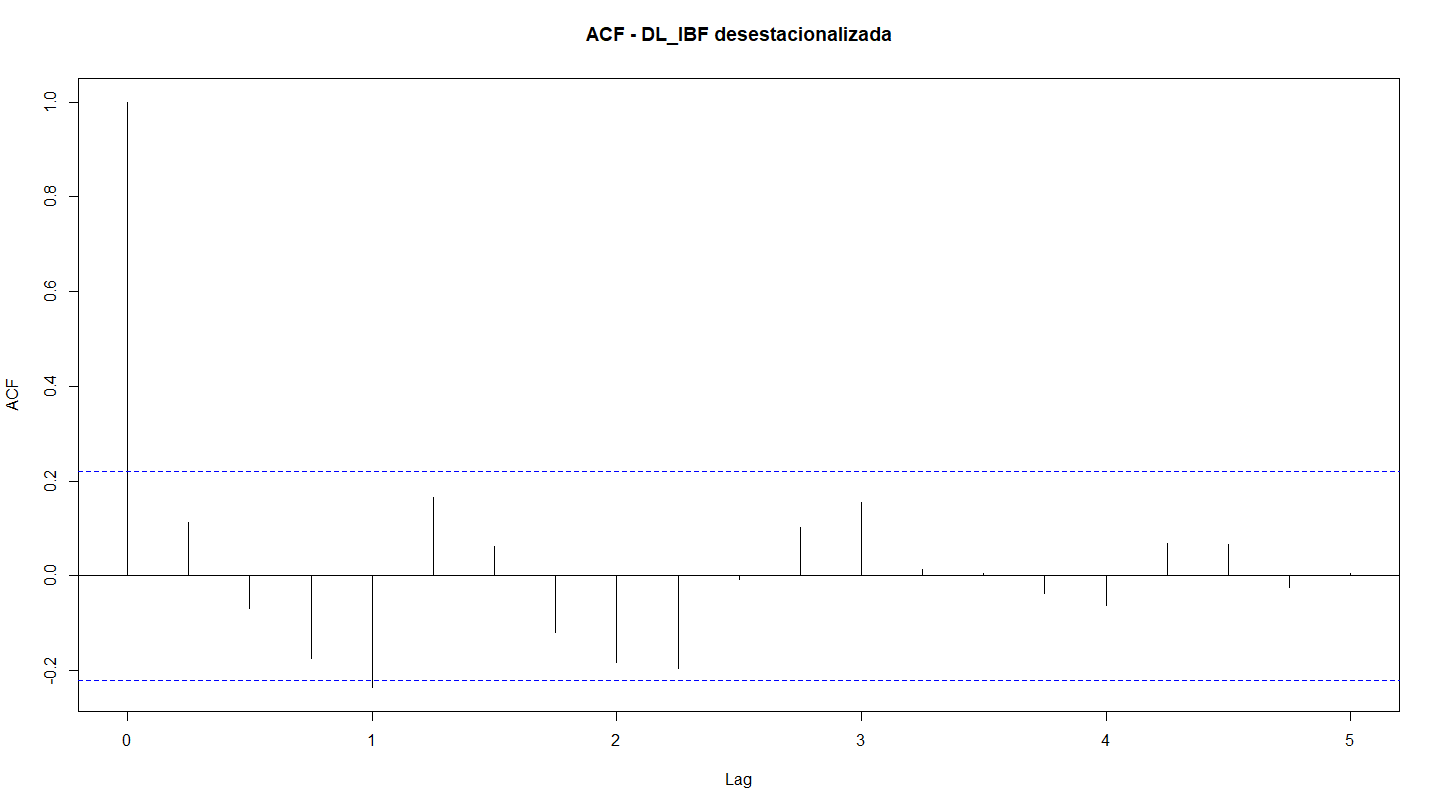
\includegraphics[width=\textwidth]{20.png}
\caption{Función de autocorrelación (ACF) de la serie DL\_IBF desestacionalizada.}
\label{fig:acf_ibf_sa}
\end{subfigure}
\hfill
\begin{subfigure}[t]{0.48\textwidth}
\centering
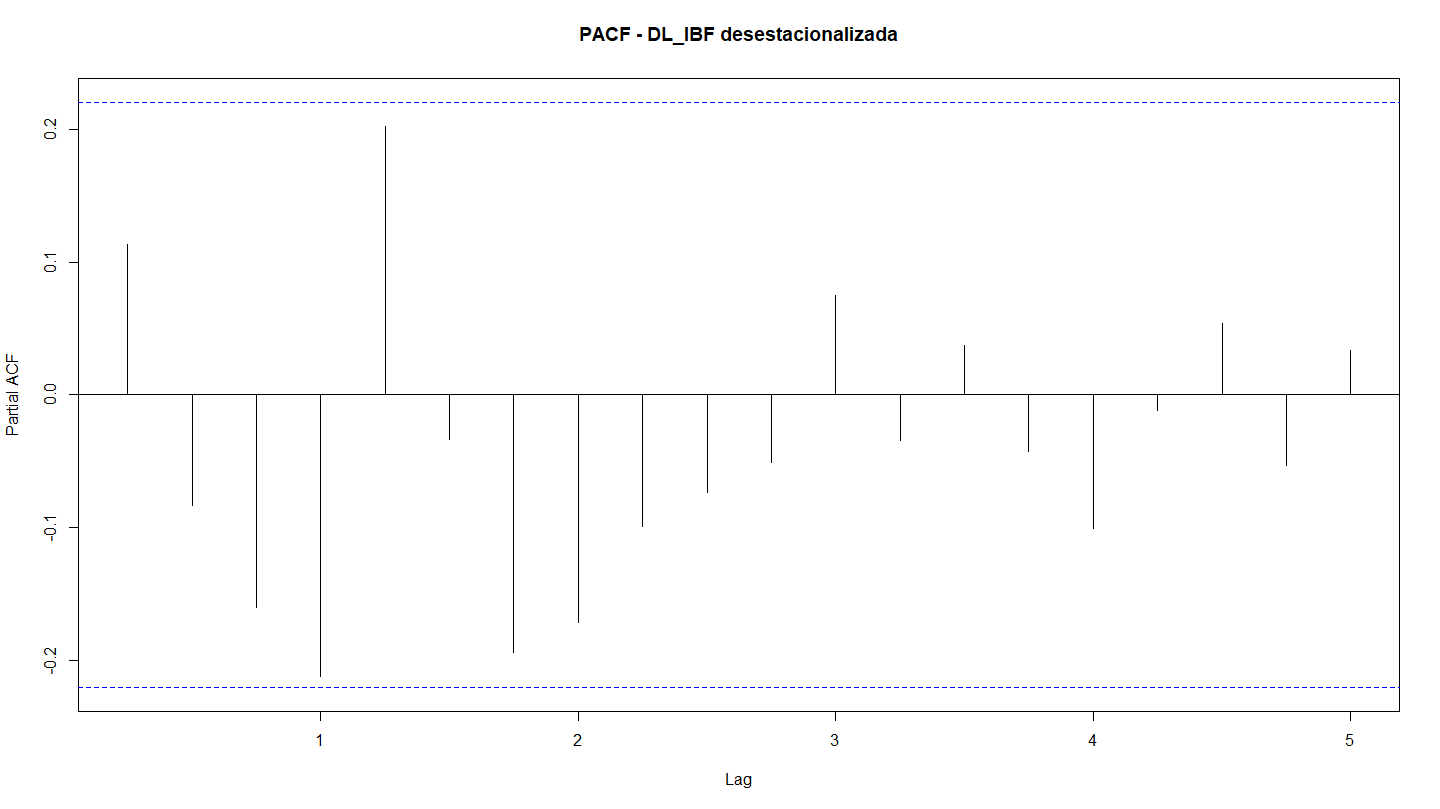
\includegraphics[width=\textwidth]{21.png}
\caption{Función de autocorrelación parcial (PACF) de la serie DL\_IBF desestacionalizada.}
\label{fig:pacf_ibf_sa}
\end{subfigure}
\end{figure}

El Cuadro~\ref{tab:arma_sa_ibf} resume la comparación entre los modelos estimados sobre la serie desestacionalizada de DL\_IBF. Los resultados muestran una tensión clara entre parsimonia estadística y capacidad de ajuste. Por un lado, el modelo automático sin media presenta el menor AIC, lo que lo favorece desde el criterio de información. Por otro lado, la especificación ARMA(0,1) obtiene los menores valores de RMSE, MAE y MASE, además de una autocorrelación residual prácticamente nula, lo que sugiere una representación más precisa de la dinámica remanente de corto plazo. El modelo de ruido blanco con media ocupa una posición intermedia en términos de error, aunque no mejora la autocorrelación residual respecto del automático. En consecuencia, aun cuando el AIC favorece al modelo automático, la evidencia conjunta de ajuste y limpieza residual sugiere que la especificación ARMA(0,1) constituye la alternativa más equilibrada para la serie ajustada. Como en otros casos, las diferencias en MAPE deben interpretarse con cautela por tratarse de una serie expresada en diferencias logarítmicas y cercana a cero.

\begin{table}[H]
\centering
\caption{Comparación de modelos ARMA sobre serie desestacionalizada – DL\_IBF}
\label{tab:arma_sa_ibf}
\resizebox{\textwidth}{!}{%
\begin{tabular}{lcccccc}
\hline
Modelo & AIC & RMSE & MAE & MAPE & MASE & ACF (res.) \\
\hline
ARMA automático (sin media) & -141.05 & 0.09784885 & 0.06845504 & 100.00 & 0.6017607 & 0.1134784 \\
Ruido blanco (con media)    & -139.63 & 0.09749049 & 0.06696559 & 127.73 & 0.5886676 & 0.1134784 \\
ARMA(0,1)                   & -138.78 & 0.09677690 & 0.06572757 & 154.50 & 0.5777846 & -0.0032673 \\
\hline
\end{tabular}%
}
\end{table}


El Cuadro~\ref{tab:diag_sa_ibf} presenta los diagnósticos residuales correspondientes a estas especificaciones. Aquí la comparación es especialmente informativa, porque el modelo automático y el ruido blanco con media arrojan p-valores inferiores a 0.05 en ambas pruebas, lo que sugiere que todavía persiste autocorrelación serial en los residuos y, por lo tanto, que esas alternativas no logran absorber completamente la dinámica de la serie desestacionalizada. En cambio, el modelo ARMA(0,1) mejora de manera visible este resultado: sus p-valores superan los niveles usuales de significatividad, de modo que no se rechaza la hipótesis de independencia residual. En consecuencia, el diagnóstico estadístico refuerza la conveniencia de privilegiar la especificación ARMA(0,1), ya que no solo exhibe mejores métricas de error dentro de la muestra, sino que además deja residuos más compatibles con un proceso de ruido blanco.

\begin{table}[H]
\centering
\caption{Diagnóstico de residuos – DL\_IBF desestacionalizada}
\begin{tabular}{lcc}
\hline
Modelo & Ljung-Box (p-valor) & Box-Ljung (p-valor) \\
\hline
ARMA automático (sin media) & 0.0458 & 0.0317 \\
Ruido blanco (con media)    & 0.0458 & 0.0317 \\
ARMA(0,1)                   & 0.0685 & 0.0952 \\
\hline
\end{tabular}
\label{tab:diag_sa_ibf}
\end{table}

La Figura~\ref{fig:forecast_ibf_ma1} presenta el pronóstico fuera de muestra obtenido a partir del modelo MA(1) estimado sobre la serie desestacionalizada de DL\_IBF. Visualmente, la trayectoria pronosticada reproduce el perfil general de oscilación alrededor de cero, pero también pone de manifiesto las dificultades para anticipar con precisión una serie tan volátil como la inversión bruta fija. En particular, el modelo logra seguir razonablemente la dirección media de la dinámica, aunque muestra desvíos frente a algunos movimientos de mayor magnitud observados en el período de prueba. Este resultado es consistente con la evidencia previa: una vez removida la estacionalidad, la serie puede describirse con una estructura parsimoniosa, pero sigue expuesta a fluctuaciones abruptas que limitan la precisión de los pronósticos de corto plazo.

\begin{figure}[H]
\centering
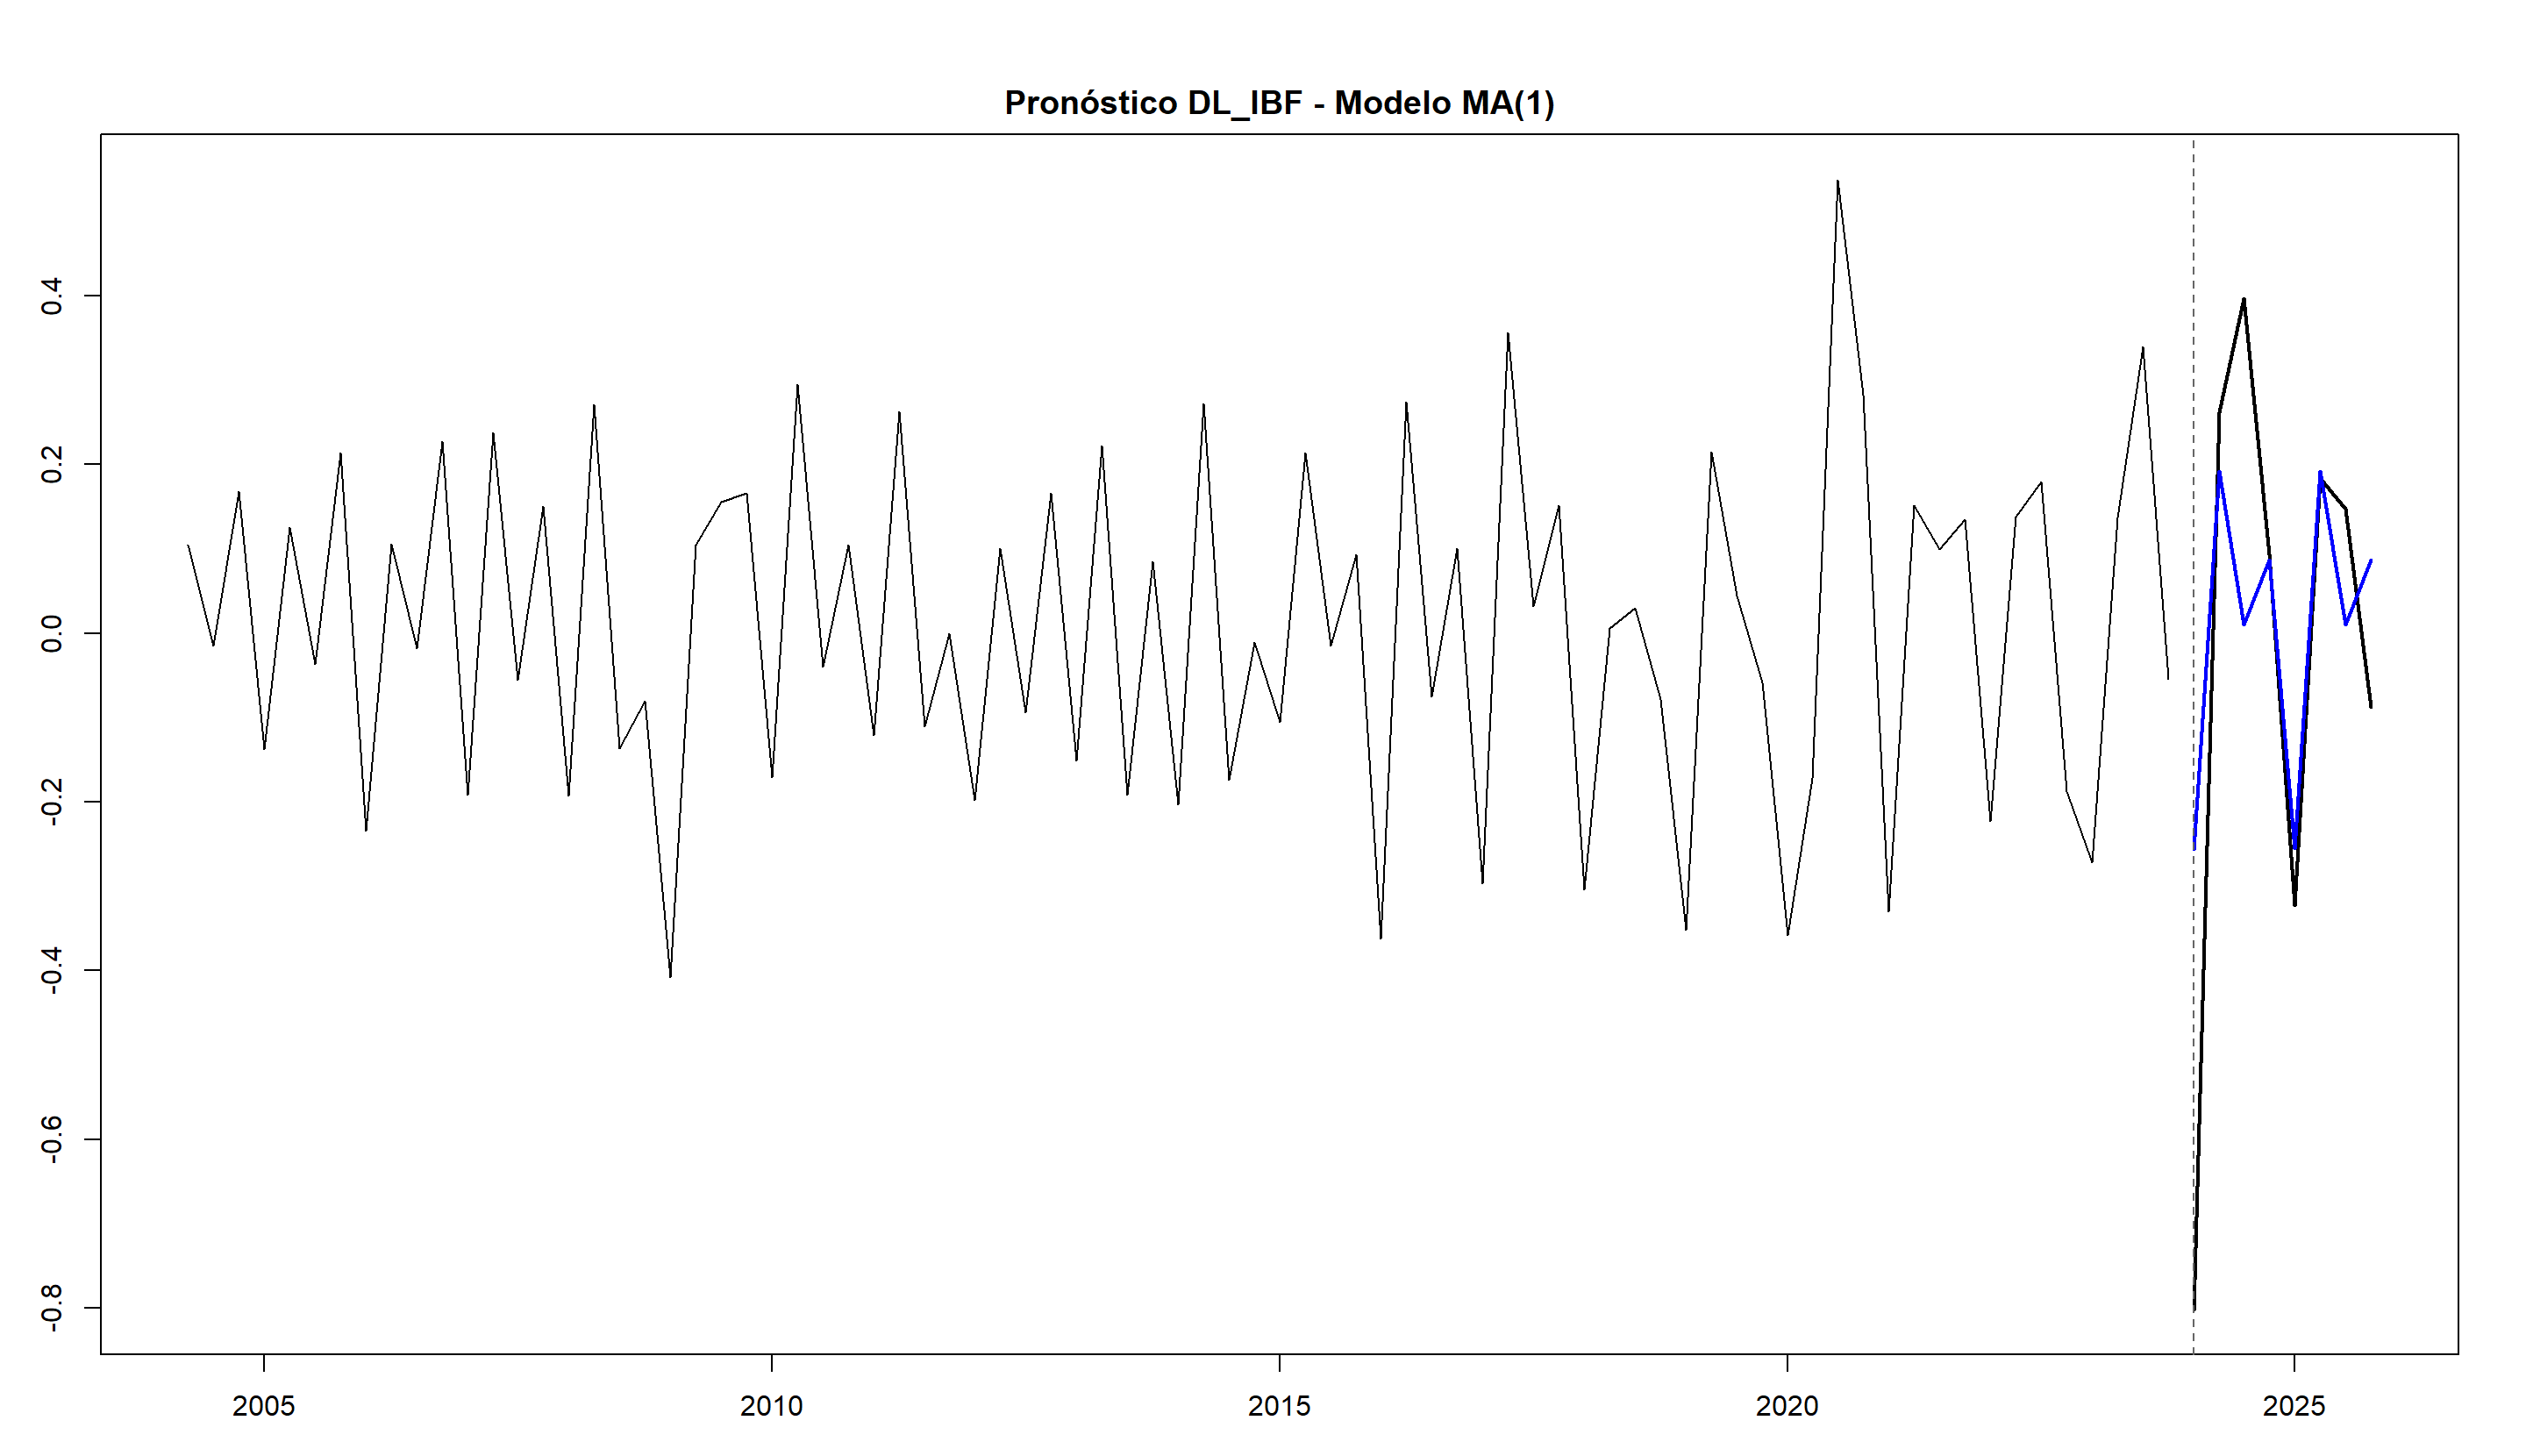
\includegraphics[width=0.95\textwidth]{22.png}
\caption{Pronóstico de la serie DL\_IBF (diferencias logarítmicas de la Inversión Bruta Fija) utilizando un modelo MA(1) estimado sobre la serie desestacionalizada. La línea negra corresponde a los valores observados (entrenamiento y valores reales), la línea azul al pronóstico y la línea vertical punteada indica el inicio del período de predicción.}
\label{fig:forecast_ibf_ma1}
\end{figure}

El Cuadro~\ref{tab:forecast_ibf_sa} reporta la evaluación cuantitativa de los pronósticos generados sobre la serie desestacionalizada. Los resultados muestran que las diferencias entre el modelo automático y la especificación MA(1) son mínimas, lo que confirma que ambas alternativas ofrecen una capacidad predictiva muy similar en este caso. El modelo automático obtiene un RMSE y un U de Theil apenas menores, mientras que el MA(1) presenta una ventaja marginal en MAE y MAPE. Sin embargo, estas diferencias son de magnitud muy reducida y no alteran la conclusión general: aun con una representación parsimoniosa y estadísticamente razonable, los modelos sobre la serie ajustada no logran una mejora predictiva clara. En consecuencia, la evidencia sugiere que, para DL\_IBF, la desestacionalización previa no genera una ganancia sustantiva en el pronóstico fuera de muestra y que las alternativas estimadas sobre la serie ajustada permanecen relativamente parejas entre sí.

\begin{table}[H]
\centering
\caption{Evaluación de pronósticos – DL\_IBF desestacionalizada}
\begin{tabular}{lcc}
\hline
Métrica & Auto & MA(1) \\
\hline
RMSE        & 0.25121435 & 0.25161206 \\
MAE         & 0.17473295 & 0.17460584 \\
MAPE        & 64.89202271 & 64.59813092 \\
U de Theil  & 0.47667328 & 0.47706045 \\
\hline
\end{tabular}
\label{tab:forecast_ibf_sa}
\end{table}

El Cuadro~\ref{tab:global_ibf} sintetiza la comparación global entre las estrategias de modelización aplicadas a DL\_IBF. La evidencia es clara en favor de los modelos SARIMA estimados sobre la serie original: en todas las métricas reportadas ---RMSE, MAE, MAPE y U de Theil--- las especificaciones con tratamiento explícito de la estacionalidad superan a las alternativas estimadas sobre la serie desestacionalizada. Dentro del grupo SARIMA, el modelo MA(1) presenta el mejor desempeño global, con los menores valores de RMSE, MAE y U de Theil, mientras que la variante AR(1) se mantiene muy próxima y el modelo automático también resulta competitivo. En cambio, los modelos sobre la serie ajustada exhiben errores sensiblemente más altos, lo que sugiere que, en el caso de la inversión bruta fija, remover previamente la estacionalidad no mejora la capacidad predictiva y puede incluso implicar pérdida de información útil para el pronóstico. Si bien el MAPE favorece también a los SARIMA en este caso, su interpretación debe seguir siendo cautelosa por la escala y naturaleza de la serie.

\begin{table}[H]
\centering
\caption{Comparación global de modelos de pronóstico – DL\_IBF}
\begin{tabular}{lccccc}
\hline
Métrica & SARIMA Auto & SARIMA MA & SARIMA AR & SA Auto & SA MA(1) \\
\hline
RMSE    & 0.20864800 & 0.20763579 & 0.20796530 & 0.25121435 & 0.25161206 \\
MAE     & 0.14895409 & 0.14855479 & 0.14870410 & 0.17473295 & 0.17460584 \\
MAPE    & 57.04265516 & 57.10475761 & 57.10214770 & 64.89202271 & 64.59813092 \\
U de Theil & 0.37951075 & 0.37676572 & 0.37762780 & 0.47667328 & 0.47706045 \\
\hline
\end{tabular}
\label{tab:global_ibf}
\end{table}

En síntesis, el análisis de la inversión bruta fija refuerza la conclusión de que la modelización directa de la estacionalidad mediante especificaciones SARIMA resulta preferible a la estrategia basada en desestacionalización previa. Aunque la serie ajustada permite trabajar con modelos ARMA simples y estadísticamente razonables, esa simplificación no se traduce en una mejora fuera de muestra. Por el contrario, los resultados sugieren que la información estacional contenida en la serie original contribuye de manera relevante a la precisión predictiva. A continuación, se desarrolla el mismo ejercicio para el producto interno bruto, una variable cuya dinámica suele ser más estable y agregada, lo que permitirá contrastar si esta conclusión se mantiene en un contexto de menor volatilidad relativa.

\subsection{Producto interno bruto (DL\_PIB)}

La Figura~\ref{fig:dl_pib} presenta la evolución de la serie DL\_PIB en diferencias logarítmicas a lo largo del período analizado. En línea con su interpretación como aproximación a la tasa de crecimiento trimestral del producto, la serie oscila alrededor de cero y exhibe una volatilidad relativamente más acotada que la observada en otras variables del trabajo, aunque con episodios puntuales de mayor amplitud. Al mismo tiempo, la trayectoria sugiere la presencia de cierta regularidad periódica, compatible con un componente estacional que conviene considerar explícitamente en la etapa de identificación del modelo.

\begin{figure}[H]
\centering
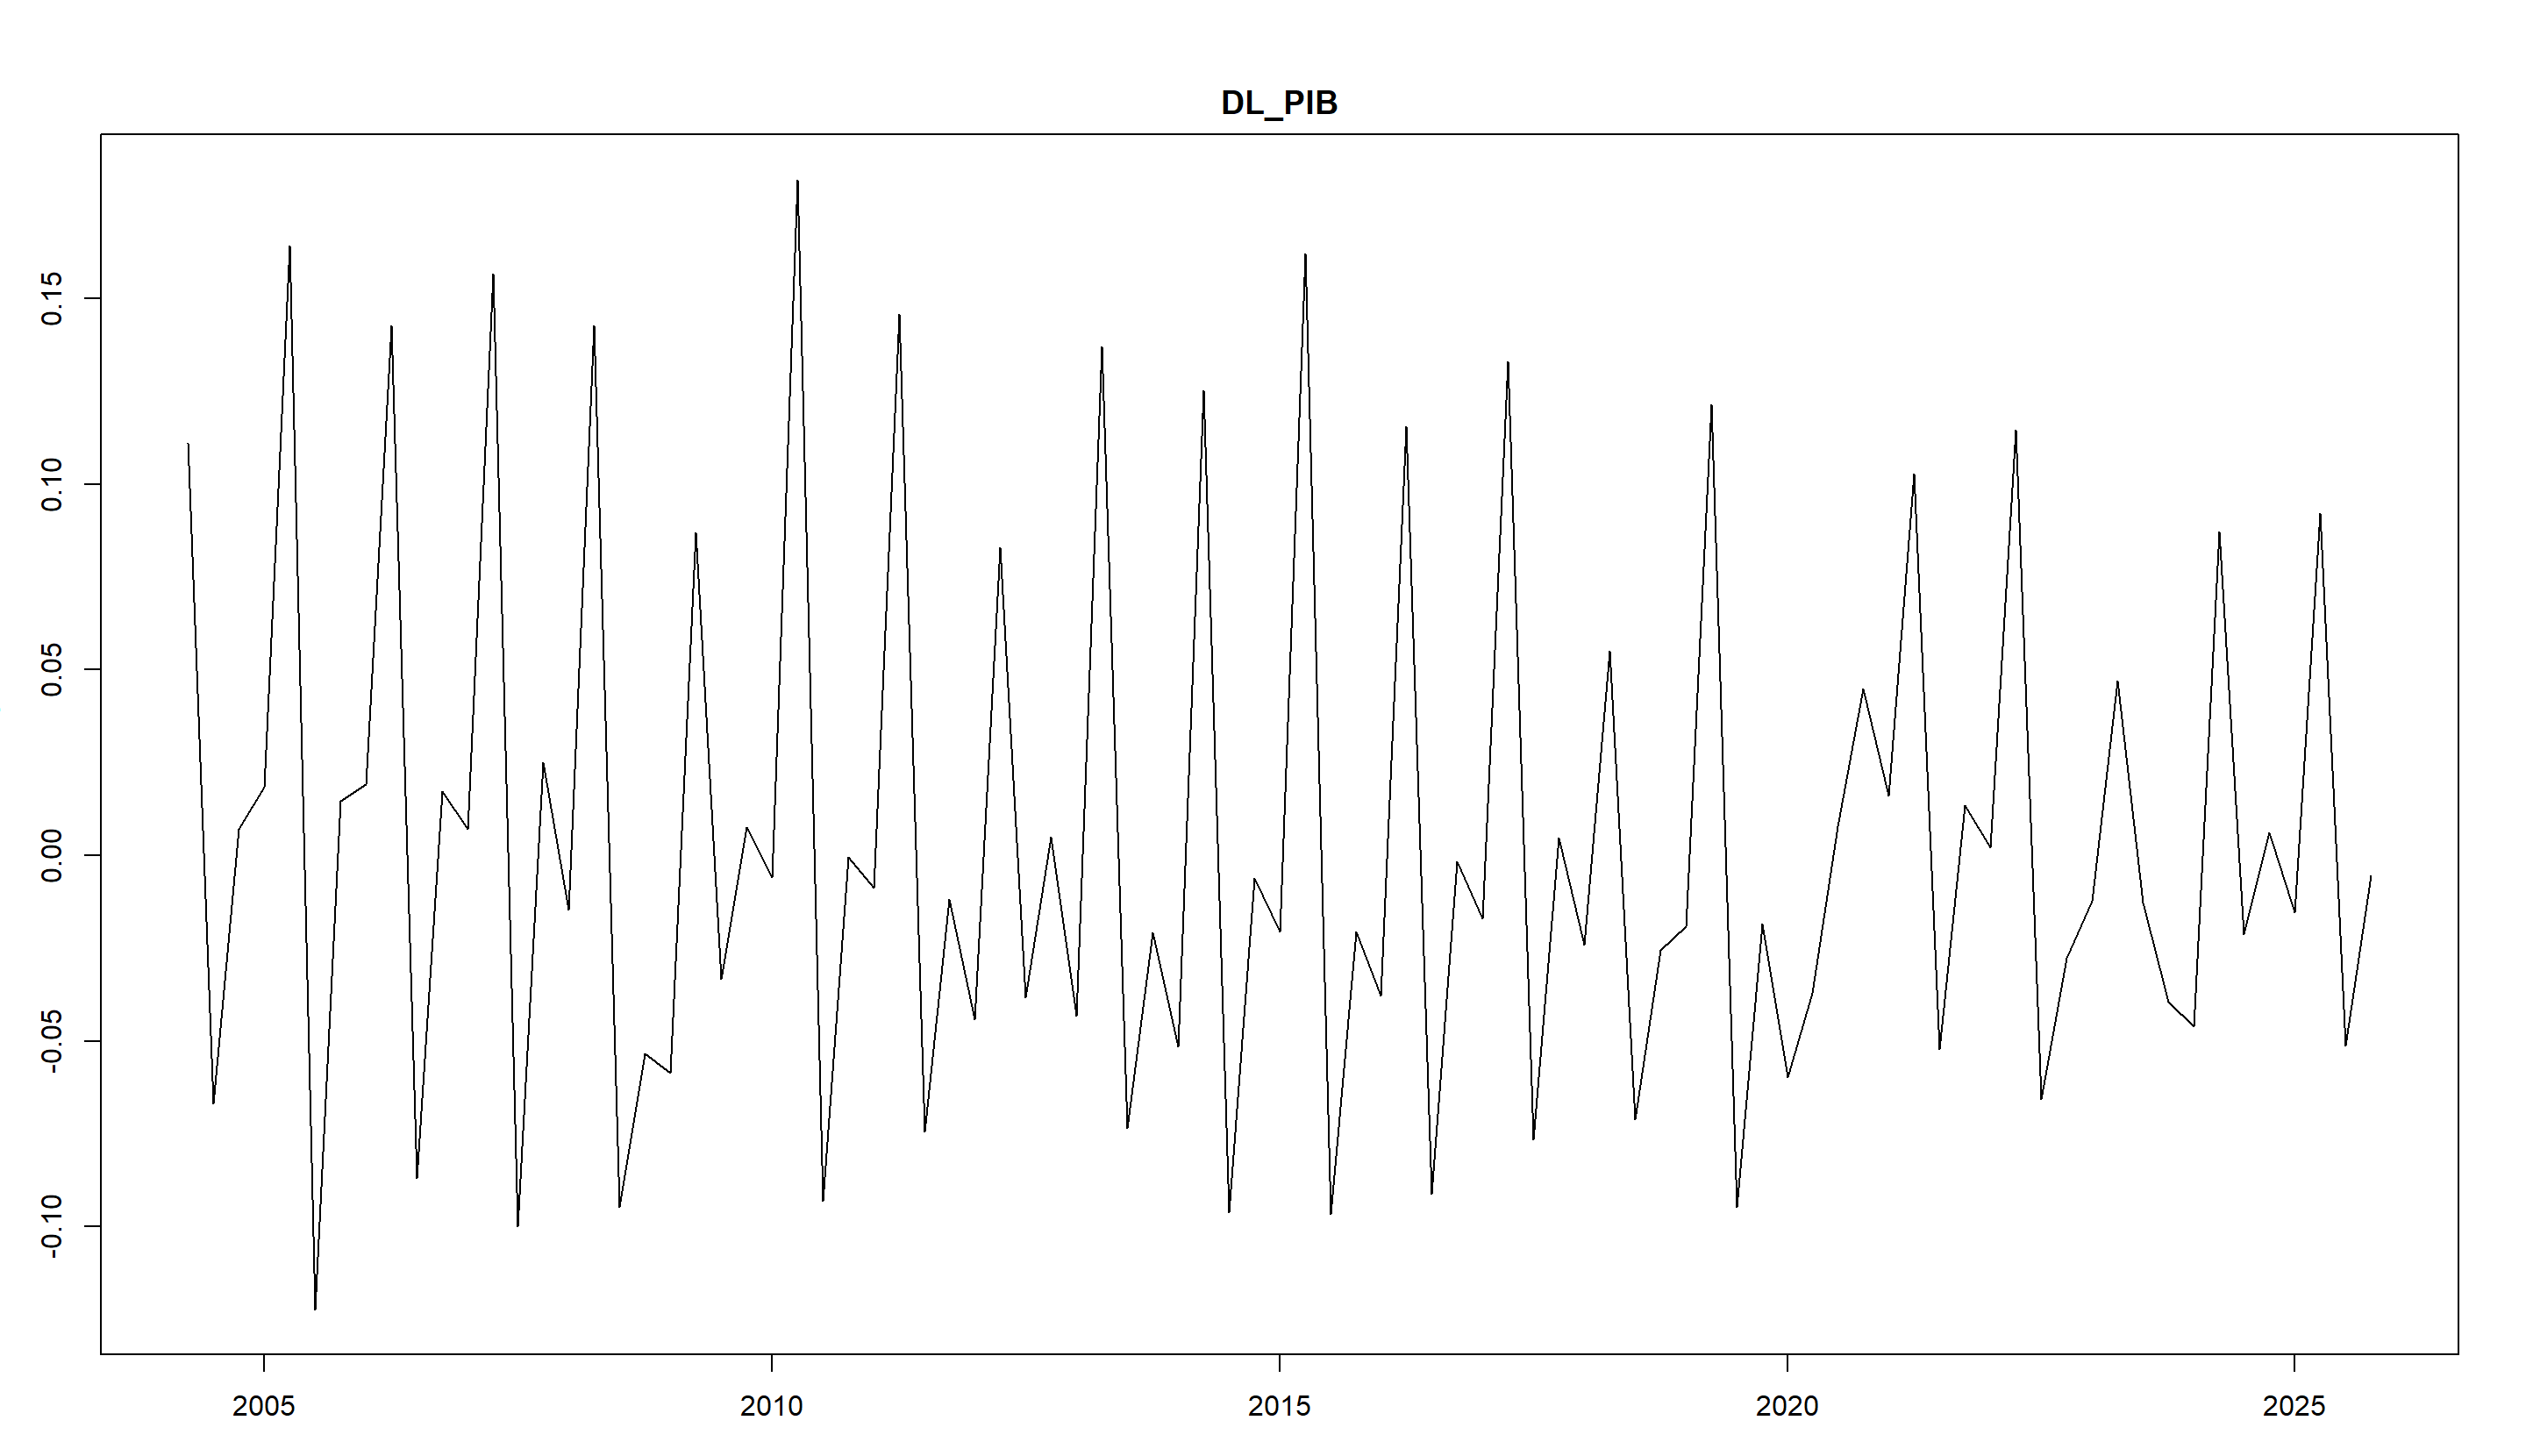
\includegraphics[width=0.95\textwidth]{23.png}
\caption{Serie DL\_PIB, correspondiente a las diferencias logarítmicas del Producto Interno Bruto (aproximación a su tasa de crecimiento trimestral), para el período 2004–2025. La serie presenta fluctuaciones alrededor de cero, con una marcada presencia de patrones estacionales y variaciones periódicas en su dinámica.}
\label{fig:dl_pib}
\end{figure}

Las Figuras~\ref{fig:acf_pib} y~\ref{fig:pacf_pib} muestran los correlogramas de autocorrelación simple y parcial de la serie original. La ACF evidencia dependencia serial en los primeros rezagos y señales en rezagos estacionales, lo que refuerza la idea de que la dinámica del PIB trimestral no es puramente transitoria y podría beneficiarse de una especificación con estructura estacional. Por su parte, la PACF presenta una pauta más concentrada en pocos rezagos relevantes, compatible con modelos de orden bajo. En conjunto, esta evidencia preliminar sugiere que una familia SARIMA parsimoniosa constituye un punto de partida natural para representar la dinámica de DL\_PIB.

\begin{figure}[H]
\centering
\begin{subfigure}[t]{0.48\textwidth}
\centering
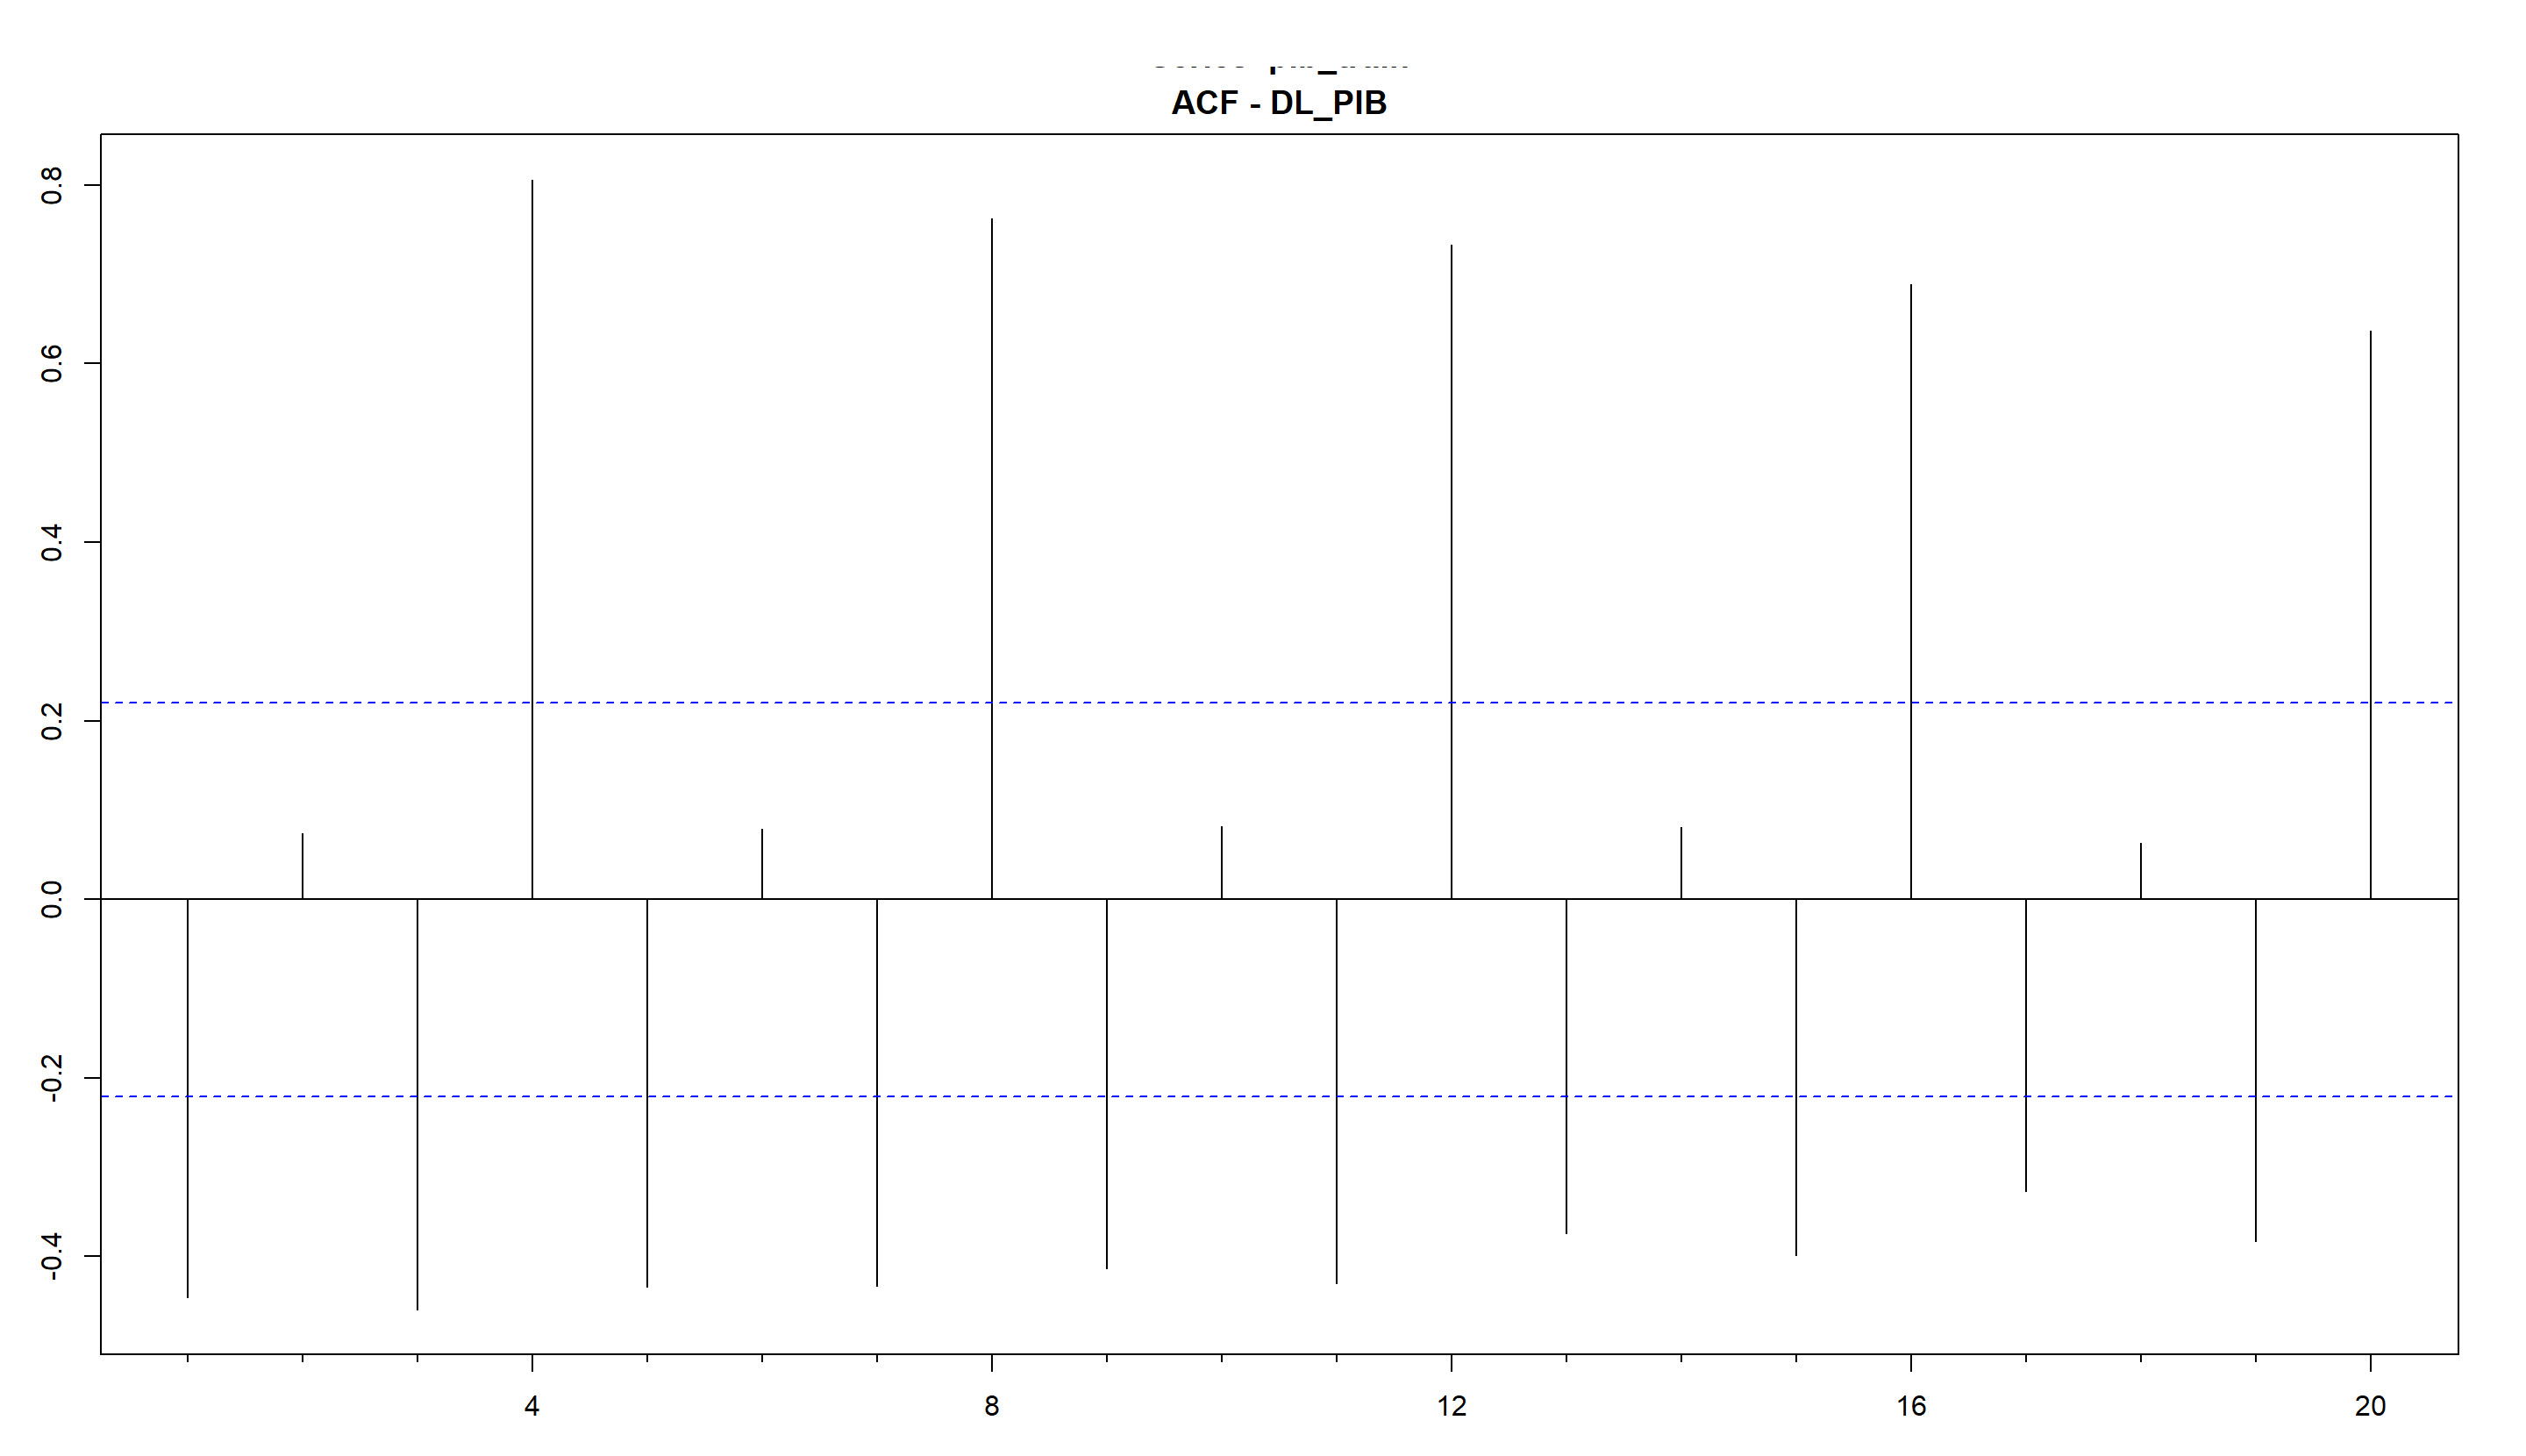
\includegraphics[width=\textwidth]{24.png}
\caption{Función de autocorrelación (ACF) de la serie DL\_PIB.}
\label{fig:acf_pib}
\end{subfigure}
\hfill
\begin{subfigure}[t]{0.48\textwidth}
\centering
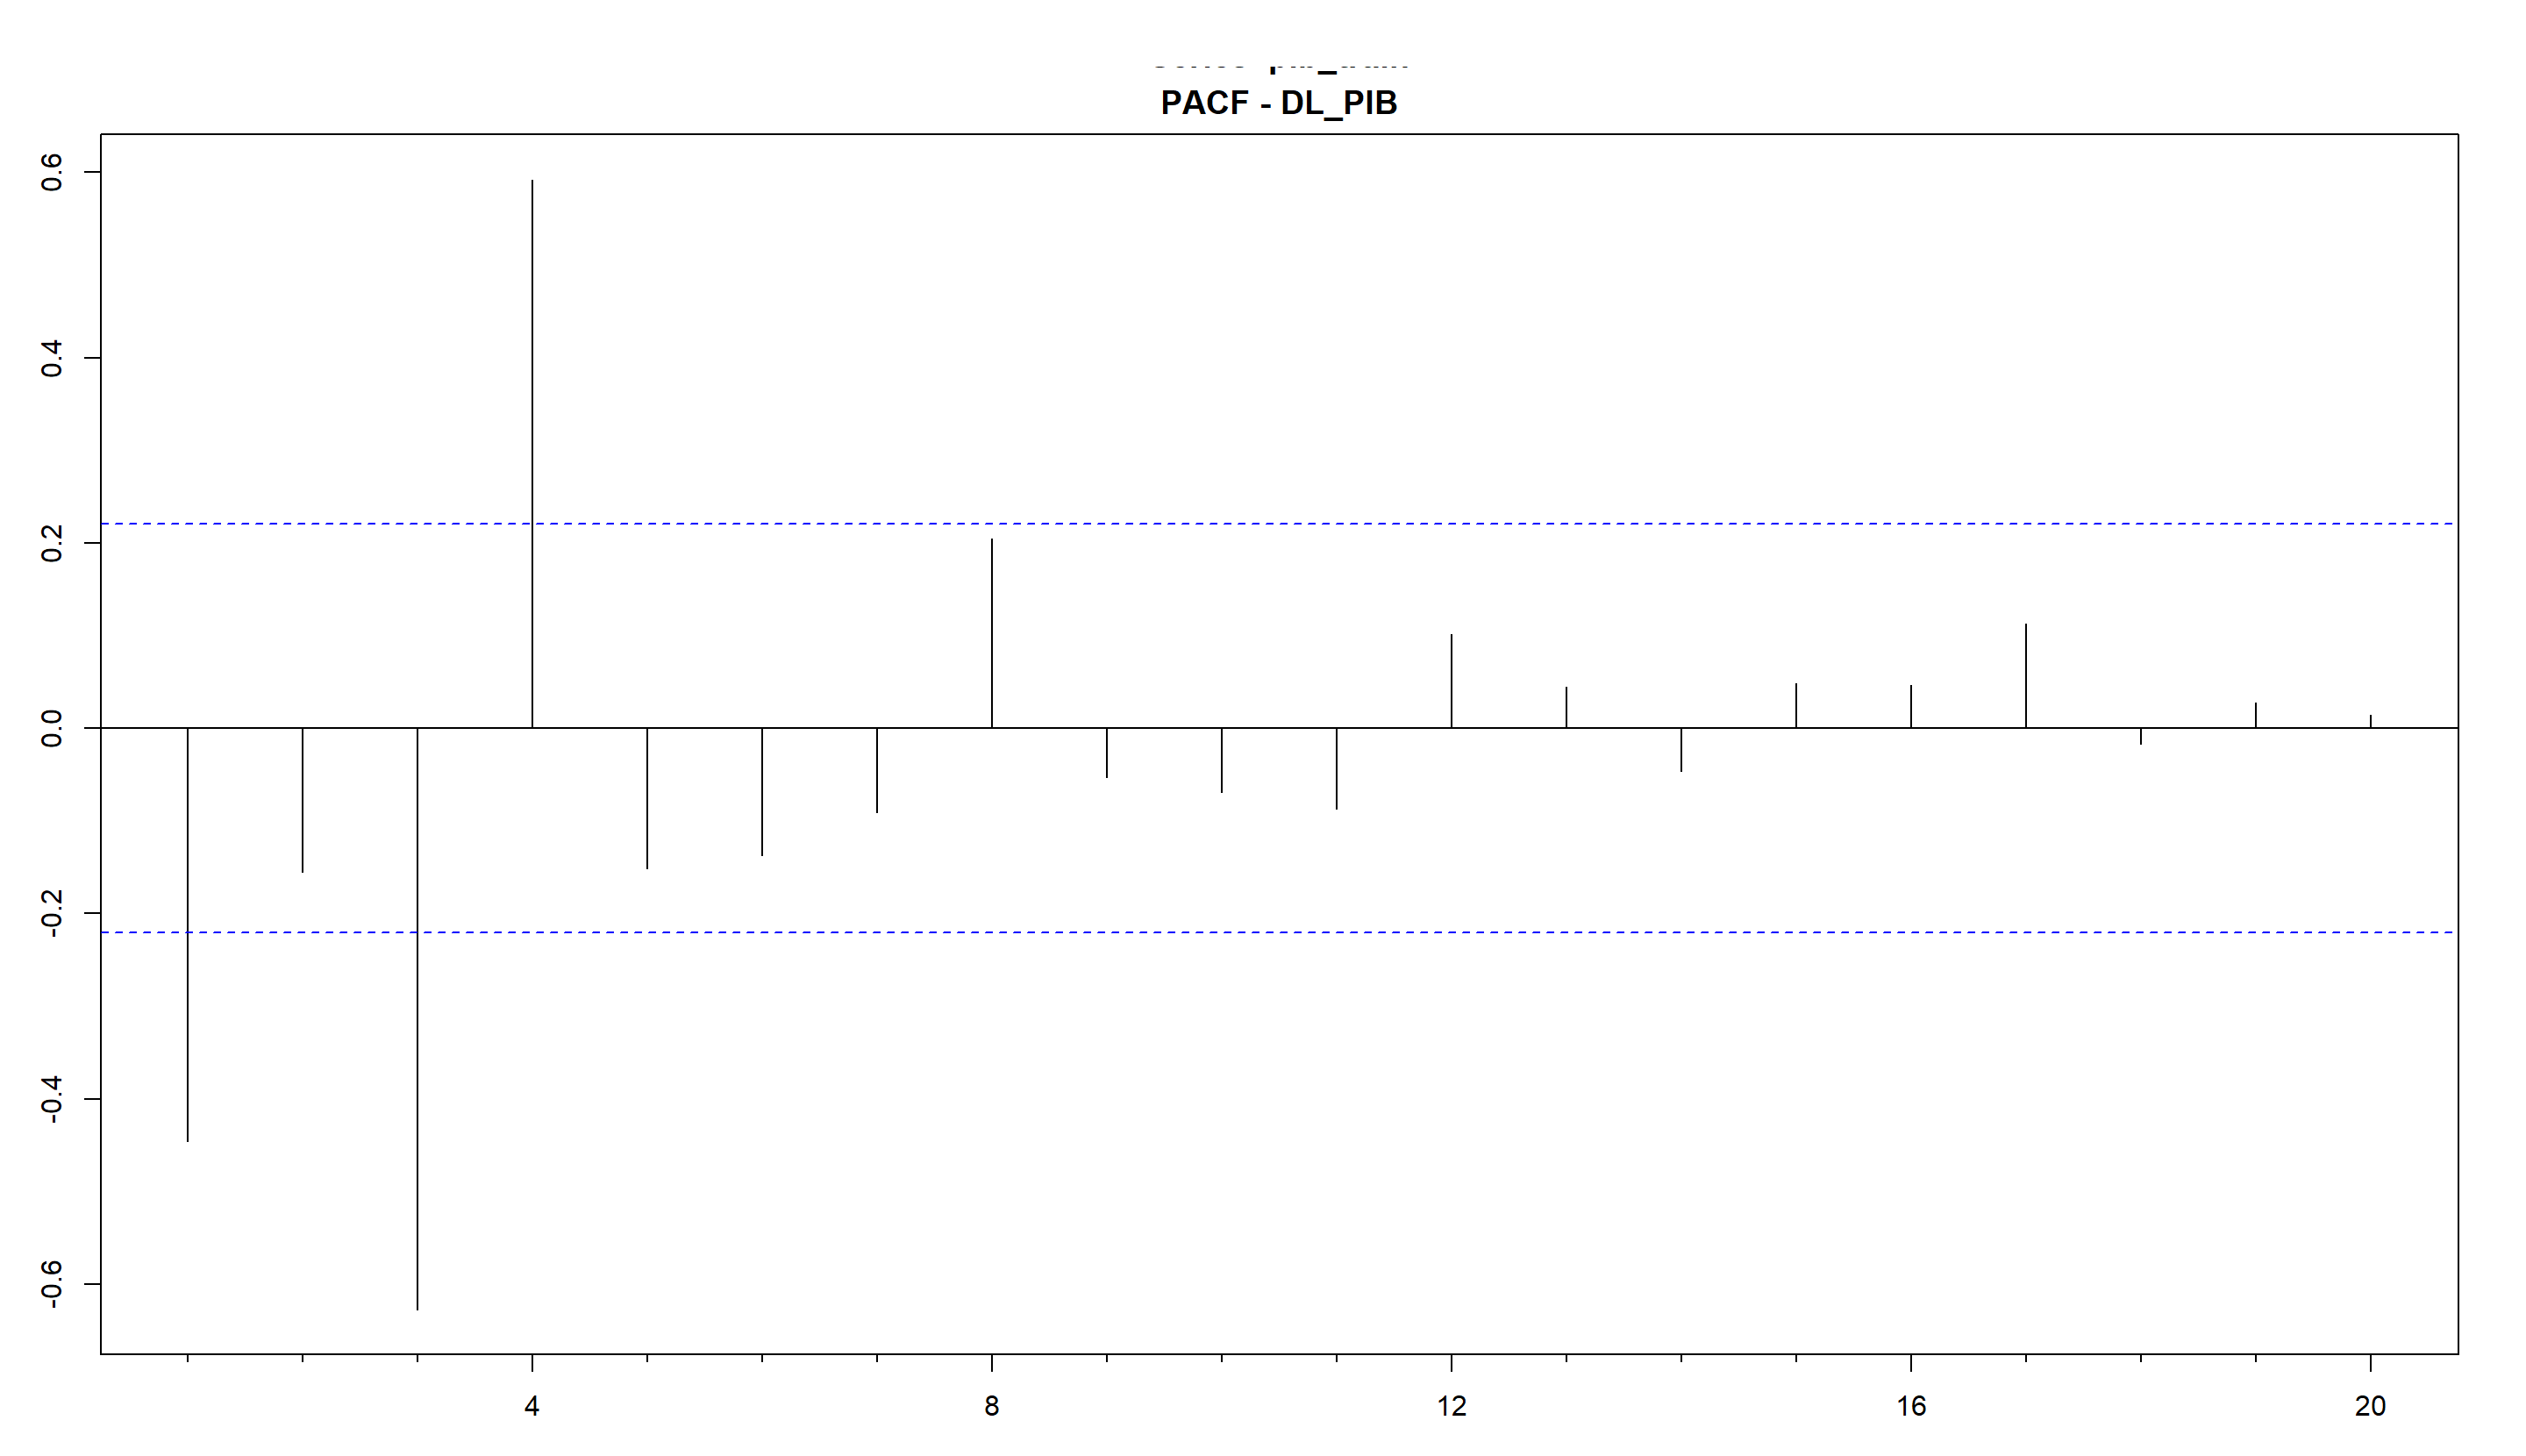
\includegraphics[width=\textwidth]{25.png}
\caption{Función de autocorrelación parcial (PACF) de la serie DL\_PIB.}
\label{fig:pacf_pib}
\end{subfigure}
\end{figure}


El Cuadro~\ref{tab:sarima_pib} resume la comparación entre las especificaciones SARIMA candidatas estimadas sobre la serie original de DL\_PIB. Los resultados muestran que las diferencias de desempeño dentro de la muestra son muy reducidas entre los tres modelos considerados, lo que sugiere que la dinámica del producto puede ser capturada adecuadamente con estructuras de baja complejidad. Aun así, la especificación automática presenta el menor AIC, lo que le otorga una ligera ventaja en términos de ajuste relativo y parsimonia. Las alternativas manuales, por su parte, exhiben métricas de error prácticamente idénticas, de modo que no aportan una mejora sustantiva frente al modelo seleccionado automáticamente.


\begin{table}[H]
\centering
\caption{Comparación de modelos SARIMA – DL\_PIB}
\label{tab:sarima_pib}
\resizebox{\textwidth}{!}{%
\begin{tabular}{lcccccc}
\hline
Modelo & AIC & RMSE & MAE & MAPE & MASE & ACF (res.) \\
\hline
SARIMA automático & -283.89 & 0.03382105 & 0.02239578 & 96.58627 & 0.664993 & -0.007387021 \\
SARIMA MA(1)      & -281.90 & 0.03382280 & 0.02239964 & 96.31495 & 0.6651078 & -0.01653204 \\
SARIMA ARMA(1,1)  & -279.90 & 0.03382310 & 0.02240327 & 95.81355 & 0.6652156 & -0.01739438 \\
\hline
\end{tabular}%
}
\end{table}

El Cuadro~\ref{tab:diag_pib} presenta los diagnósticos residuales de los modelos estimados para DL\_PIB. En todos los casos, los p-valores de las pruebas de Ljung-Box y Box-Ljung son elevados, lo que indica que no queda evidencia relevante de autocorrelación serial en los residuos y que las tres especificaciones resultan estadísticamente admisibles. En este sentido, el modelo automático vuelve a destacarse levemente, al combinar el mejor criterio de información con un diagnóstico residual particularmente sólido. En conjunto, la evidencia sugiere que cualquiera de las alternativas consideradas describe razonablemente bien la dependencia temporal de la serie, aunque la especificación automática conserva una pequeña ventaja como referencia inicial para la etapa de pronóstico.

\begin{table}[H]
\centering
\caption{Diagnóstico de residuos – DL\_PIB}
\label{tab:diag_pib}
\begin{tabular}{lcc}
\hline
Modelo & Ljung-Box (p-valor) & Box-Ljung (p-valor) \\
\hline
SARIMA automático & 0.9336 & 0.8756 \\
SARIMA MA(1)      & 0.8820 & 0.8750 \\
SARIMA ARMA(1,1)  & 0.7928 & 0.8713 \\
\hline
\end{tabular}
\end{table}

La Figura~\ref{fig:forecast_pib_sarima} compara los pronósticos fuera de muestra generados por las tres especificaciones SARIMA consideradas para DL\_PIB. Visualmente, las trayectorias pronosticadas son muy similares entre sí y reproducen una dinámica relativamente estable, con oscilaciones acotadas alrededor de cero, en línea con la menor volatilidad observada para el producto en comparación con otras series del trabajo. Las bandas de confianza también resultan bastante próximas, lo que sugiere que las diferencias entre modelos son sutiles y que todos capturan de manera semejante la evolución esperada de corto plazo. Dentro de esa alta similitud, la especificación ARMA(1,1) parece ajustarse levemente mejor a algunos movimientos observados en el período de prueba, aunque la ventaja visual respecto de las demás alternativas es moderada.

\begin{figure}[H]
\centering
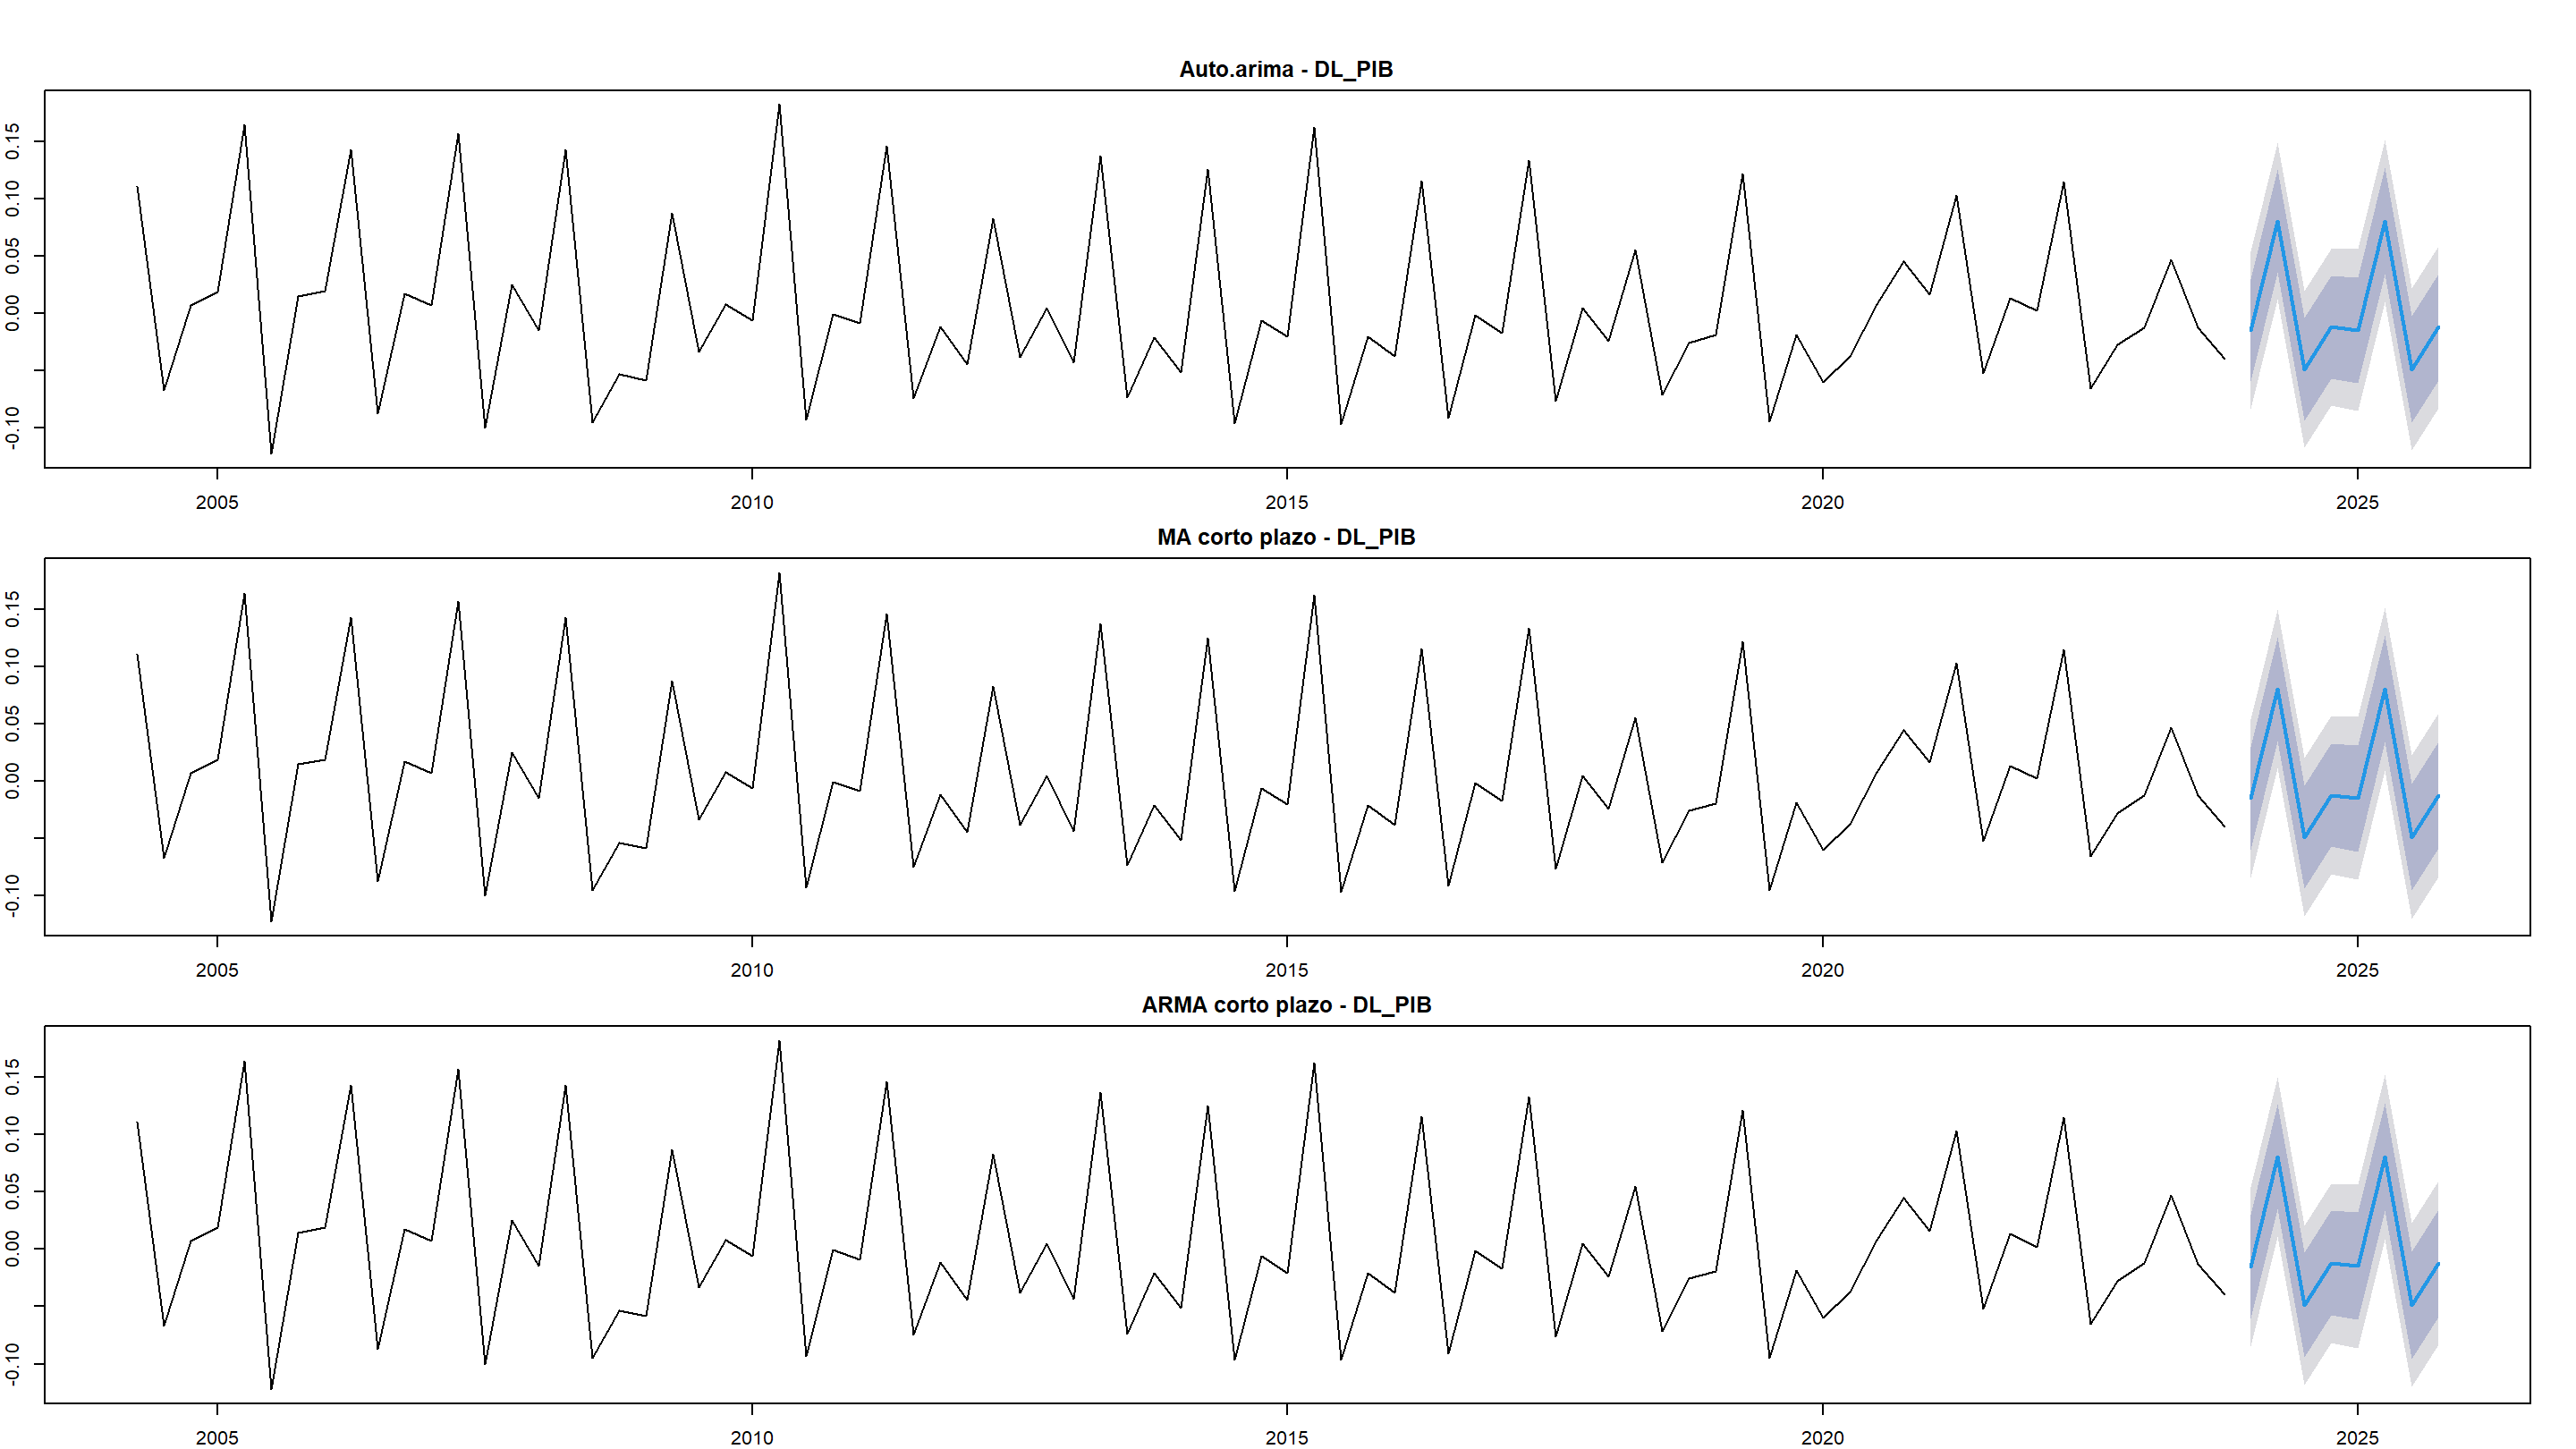
\includegraphics[width=0.95\textwidth]{26.png}
\caption{Comparación de pronósticos para la serie DL\_PIB bajo distintas especificaciones SARIMA. La línea negra corresponde a los valores observados, las líneas azules a los pronósticos y las bandas sombreadas representan los intervalos de confianza. La línea vertical punteada indica el inicio del período de predicción.}
\label{fig:forecast_pib_sarima}
\end{figure}


El Cuadro~\ref{tab:forecast_pib} presenta la evaluación cuantitativa del desempeño predictivo fuera de muestra para el período 2024--2025. Los resultados muestran nuevamente diferencias muy pequeñas entre las tres especificaciones, lo que confirma que la capacidad predictiva de los modelos SARIMA para DL\_PIB es bastante similar en términos prácticos. No obstante, la especificación SARIMA ARMA(1,1) obtiene los mejores valores en RMSE, MAE, MAPE y U de Theil, seguida muy de cerca por el modelo MA(1), mientras que la variante automática queda apenas por detrás. En consecuencia, la evidencia fuera de muestra sugiere una ventaja marginal para el modelo ARMA(1,1), aunque de magnitud reducida. Como en otras series expresadas en diferencias logarítmicas, el MAPE debe interpretarse con cautela, dado que los valores cercanos a cero tienden a amplificar esta métrica relativa.


\begin{table}[H]
\centering
\caption{Evaluación de desempeño predictivo (fuera de muestra) – DL\_PIB}
\label{tab:forecast_pib}
\begin{tabular}{lcccc}
\hline
Modelo & RMSE & MAE & MAPE & U de Theil \\
\hline
SARIMA automático & 0.01687517 & 0.01304243 & 79.53992737 & 0.16878746 \\
SARIMA MA(1)      & 0.01680381 & 0.01302810 & 79.57194804 & 0.16814761 \\
SARIMA ARMA(1,1)  & 0.01673073 & 0.01295910 & 79.41645092 & 0.16730119 \\
\hline
\end{tabular}
\end{table}


La Figura~\ref{fig:dl_pib_sa} presenta la serie DL\_PIB una vez removido el componente estacional mediante el procedimiento X-13. En comparación con la serie original, la trayectoria desestacionalizada conserva un comportamiento relativamente estable y fluctuaciones acotadas alrededor de cero, aunque permite observar con mayor nitidez los movimientos de corto plazo no asociados al patrón trimestral regular. La serie sigue mostrando algunos episodios de mayor volatilidad, en particular alrededor de 2020, pero en términos generales la desestacionalización sugiere que buena parte de la dinámica remanente del producto responde a variaciones transitorias de baja amplitud. En este sentido, la versión ajustada ofrece una base adecuada para evaluar si una especificación no estacional simple puede capturar satisfactoriamente la persistencia restante.

\begin{figure}[H]
\centering
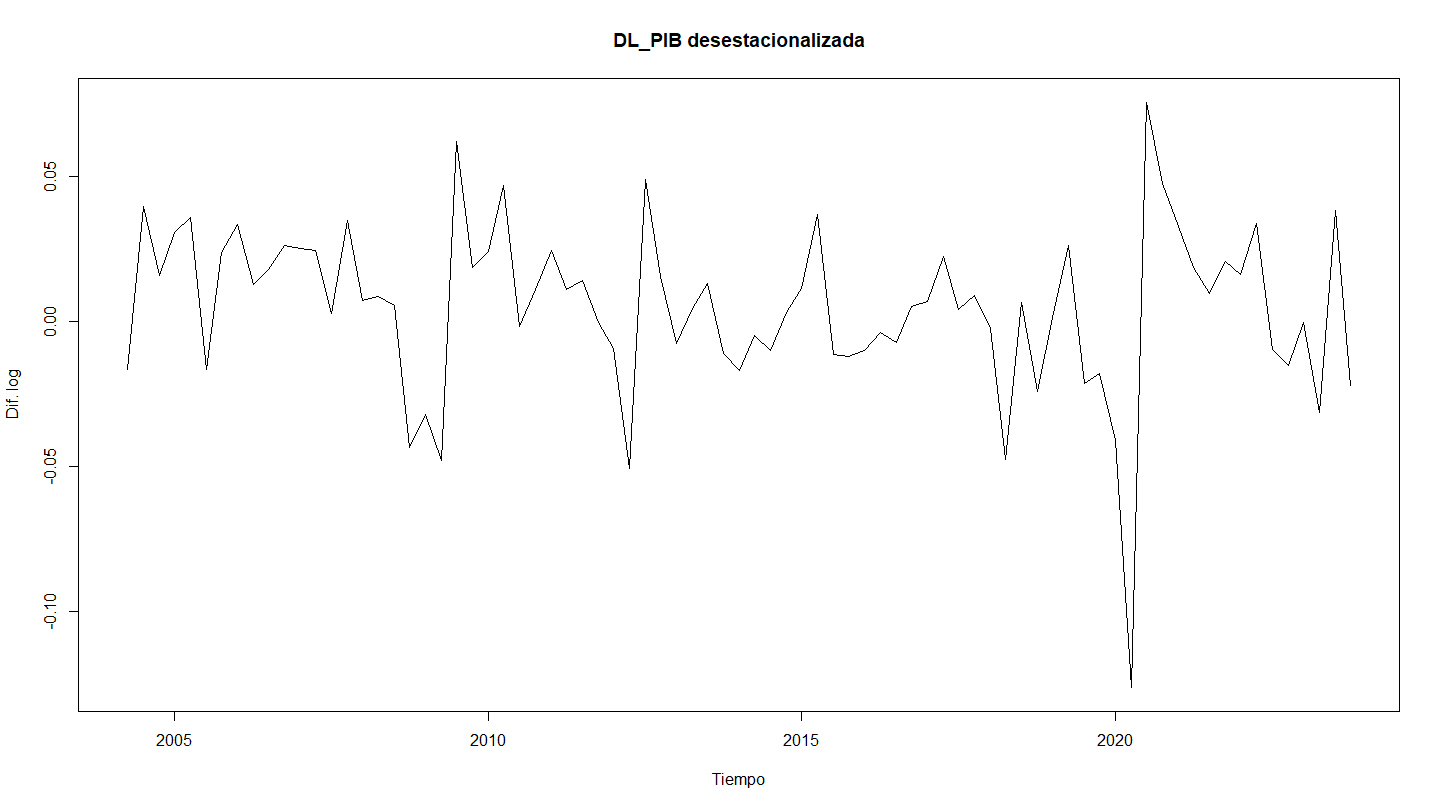
\includegraphics[width=0.95\textwidth]{27.png}
\caption{Serie DL\_PIB desestacionalizada. Se observa la dinámica de corto plazo sin componente estacional, destacándose episodios de mayor volatilidad, particularmente alrededor de 2020.}
\label{fig:dl_pib_sa}
\end{figure}

Las Figuras~\ref{fig:acf_pib_sa} y~\ref{fig:pacf_pib_sa} muestran los correlogramas de la serie desestacionalizada. A diferencia de lo observado en la serie original, la ACF exhibe una dependencia serial más tenue y sin un patrón estacional marcado, lo que indica que la remoción del componente periódico simplifica de manera importante la estructura temporal del PIB. Por su parte, la PACF presenta una pauta bastante acotada, con pocos rezagos potencialmente relevantes y sin señales de una dinámica compleja. En conjunto, la evidencia gráfica sugiere que, una vez desestacionalizada la serie, la dinámica remanente puede ser razonablemente aproximada mediante modelos ARMA de bajo orden, e incluso abre la posibilidad de considerar especificaciones muy parsimoniosas.

\begin{figure}[H]
\centering
\begin{subfigure}[t]{0.48\textwidth}
\centering
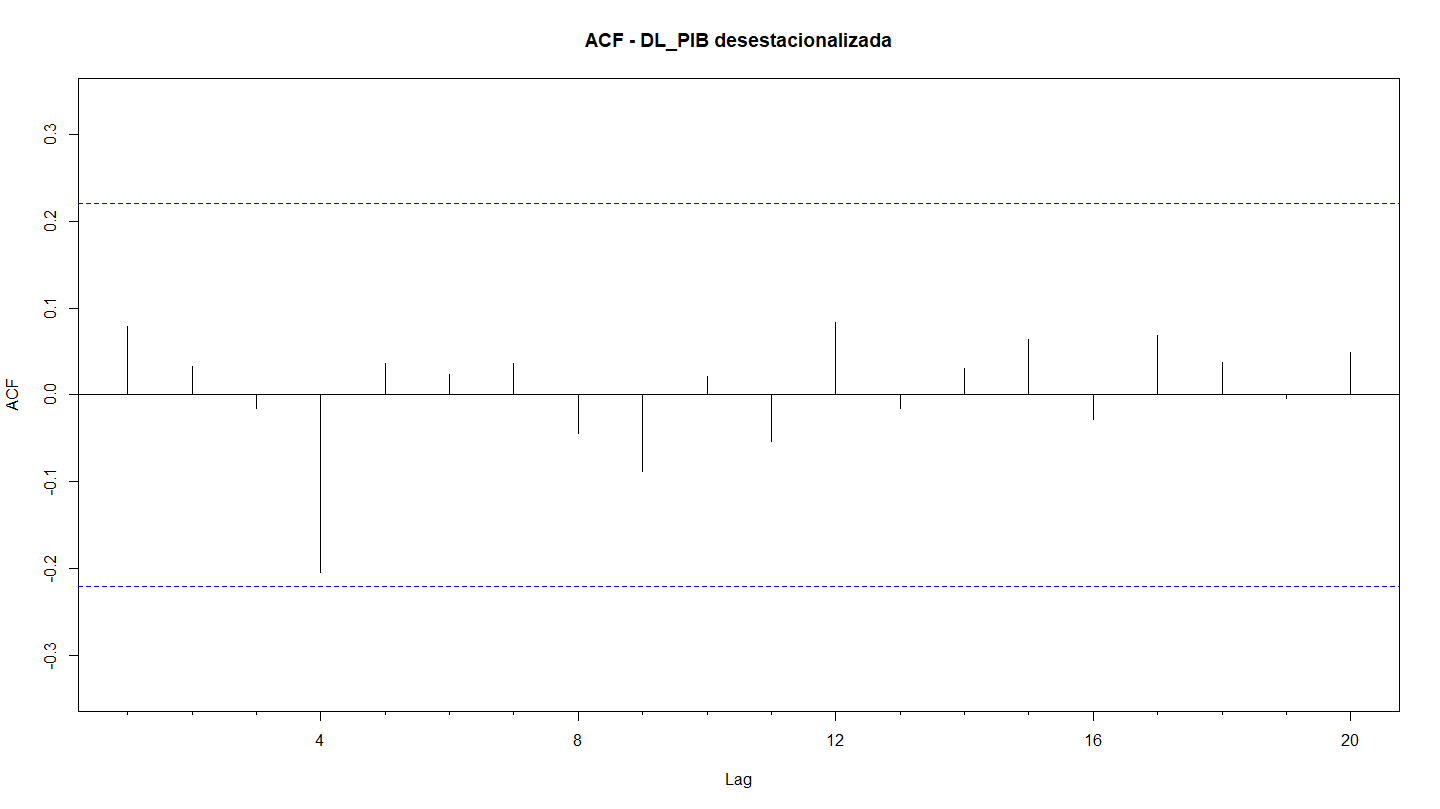
\includegraphics[width=\textwidth]{28.png}
\caption{Función de autocorrelación (ACF) de la serie DL\_PIB desestacionalizada.}
\label{fig:acf_pib_sa}
\end{subfigure}
\hfill
\begin{subfigure}[t]{0.48\textwidth}
\centering
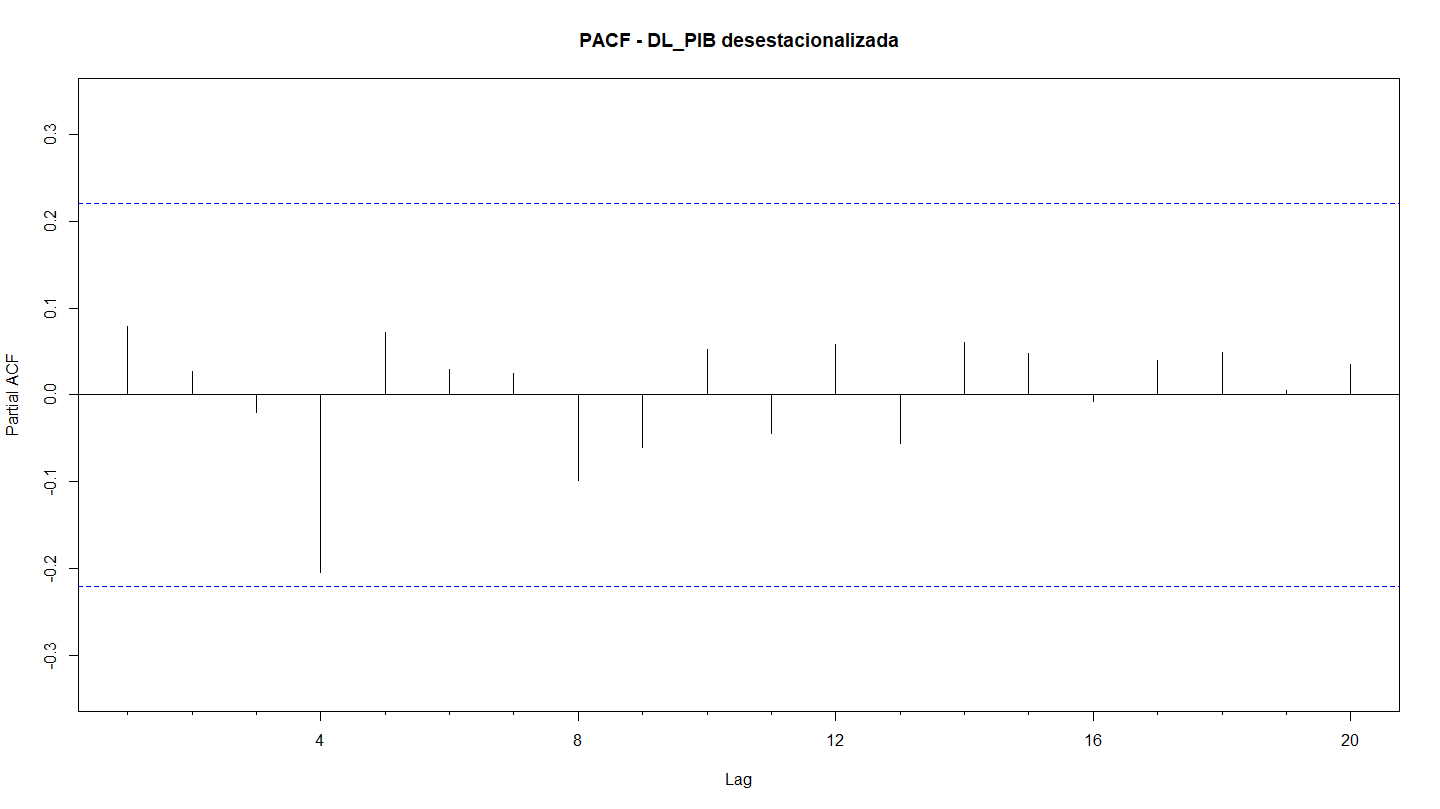
\includegraphics[width=\textwidth]{29.png}
\caption{Función de autocorrelación parcial (PACF) de la serie DL\_PIB desestacionalizada.}
\label{fig:pacf_pib_sa}
\end{subfigure}
\end{figure}

El Cuadro~\ref{tab:arma_dl_pib} resume la comparación entre los modelos estimados sobre la serie desestacionalizada de DL\_PIB. Un primer resultado relevante es que el modelo automático coincide con un proceso de ruido blanco con media, lo que sugiere que, una vez removida la estacionalidad, la persistencia remanente del producto es relativamente débil. Al mismo tiempo, la especificación ARMA(0,1) exhibe mejoras marginales en RMSE, MAE, MAPE, MASE y autocorrelación residual, aunque a costa de un AIC ligeramente menos favorable. En consecuencia, el cuadro muestra una disyuntiva acotada entre parsimonia y pequeñas ganancias de ajuste: si se prioriza el criterio de información, el modelo automático aparece como referencia natural; si se privilegia una mejora, aunque tenue, en las métricas de error y en la limpieza residual, el ARMA(0,1) surge como una alternativa competitiva.

\begin{table}[H]
\centering
\caption{Comparación de modelos ARMA sobre serie desestacionalizada – DL\_PIB}
\resizebox{\textwidth}{!}{%
\begin{tabular}{lcccccc}
\hline
Modelo & AIC & RMSE & MAE & MAPE & MASE & ACF (res.) \\
\hline
ARMA automático (con media) & -330.64 & 0.02910256 & 0.02120466 & 137.2988 & 0.6331323 & 0.07866753 \\
Ruido blanco (con media)    & -330.64 & 0.02910256 & 0.02120466 & 137.2988 & 0.6331323 & 0.07866753 \\
ARMA(0,1)                   & -329.11 & 0.02901554 & 0.02091538 & 134.8073 & 0.6244946 & 0.002521403 \\
\hline
\end{tabular}%
}
\label{tab:arma_dl_pib}
\end{table}

El Cuadro~\ref{tab:diag_sa_pib} presenta los diagnósticos residuales correspondientes a estas especificaciones. Los p-valores de las pruebas de Ljung-Box y Box-Ljung son elevados en todos los casos, por lo que no hay evidencia de autocorrelación serial remanente y las tres alternativas resultan estadísticamente admisibles. A diferencia de otras series más volátiles, aquí incluso las especificaciones más simples superan holgadamente los tests de independencia, lo que refuerza la idea de que la desestacionalización deja una dinámica particularmente tenue. En este contexto, el diagnóstico residual no obliga a descartar ninguna opción: el modelo automático y el ruido blanco con media conservan una ventaja por simplicidad, mientras que el ARMA(0,1) puede justificarse si se desea capturar una dependencia muy leve sin comprometer la calidad estadística de los residuos.

\begin{table}[H]
\centering
\caption{Diagnóstico de residuos – DL\_PIB desestacionalizada}
\begin{tabular}{lcc}
\hline
Modelo & Ljung-Box (p-valor) & Box-Ljung (p-valor) \\
\hline
ARMA automático (con media) & 0.7941 & 0.8981 \\
Ruido blanco (con media)    & 0.7941 & 0.8981 \\
ARMA(0,1)                   & 0.7428 & 0.9027 \\
\hline
\end{tabular}
\label{tab:diag_sa_pib}
\end{table}

La Figura~\ref{fig:forecast_pib_sa_models} compara los pronósticos fuera de muestra generados por las tres especificaciones estimadas sobre la serie desestacionalizada de DL\_PIB. Visualmente, las trayectorias pronosticadas son muy parecidas entre sí y reproducen una dinámica relativamente suave, coherente con la menor volatilidad que presenta el producto una vez removido el componente estacional. El modelo automático y el ruido blanco con media producen trayectorias idénticas, lo que refleja nuevamente que la selección automática no detecta una estructura dinámica adicional relevante en la serie ajustada. La especificación MA(1), por su parte, introduce una leve mejora en el seguimiento de algunos movimientos observados durante el período de prueba, aunque las diferencias respecto de las otras alternativas siguen siendo acotadas. En conjunto, la figura sugiere que la desestacionalización deja una dinámica suficientemente simple como para que modelos muy parsimoniosos generen pronósticos bastante similares.

\begin{figure}[H]
\centering
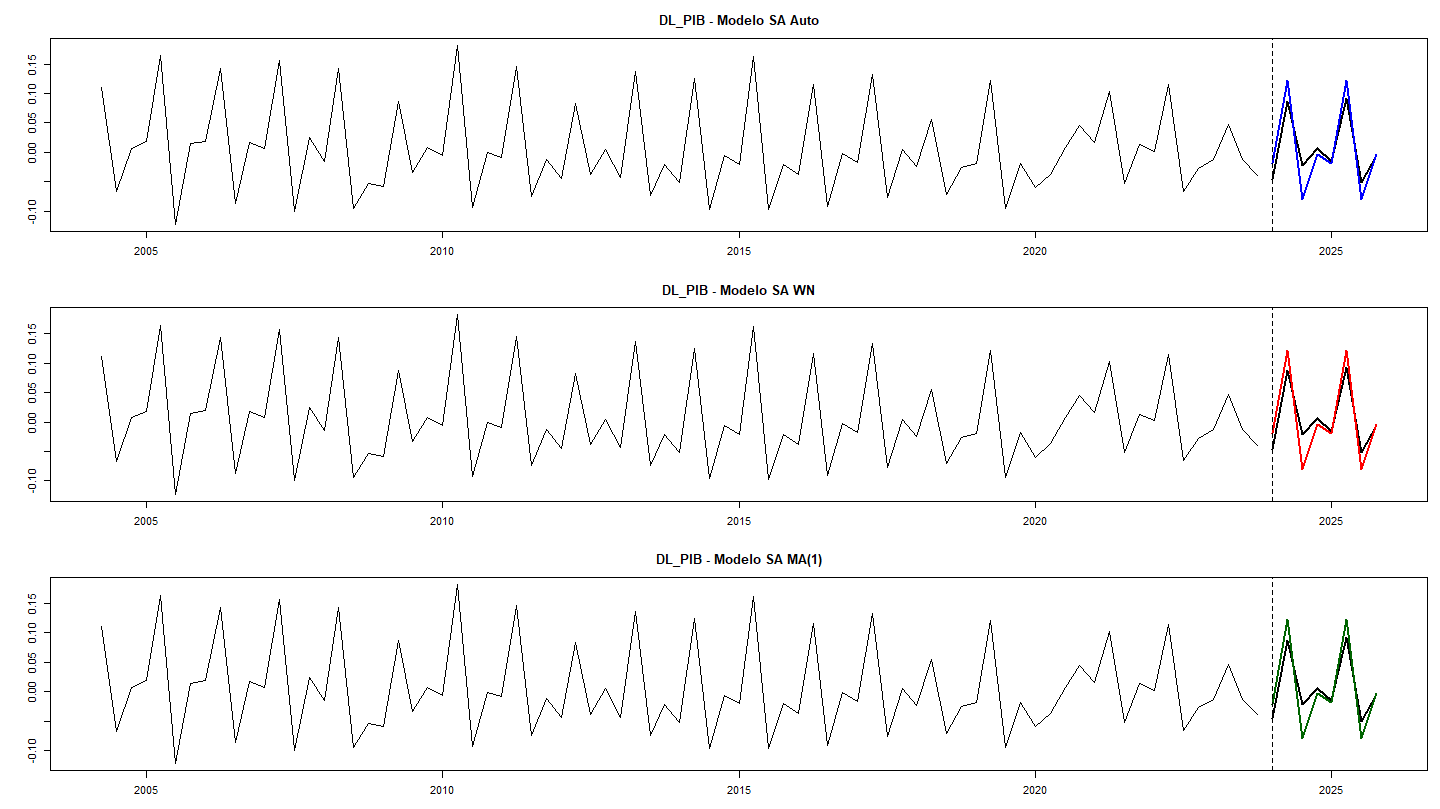
\includegraphics[width=0.95\textwidth]{30.png}
\caption{Pronósticos fuera de muestra para la serie DL\_PIB bajo tres especificaciones sobre la serie desestacionalizada. Cada panel muestra el ajuste del modelo sobre la muestra de entrenamiento (línea negra), los valores observados en el período de prueba (línea negra posterior al corte) y los pronósticos generados (líneas de color). La línea vertical punteada indica el inicio del horizonte de predicción.}
\label{fig:forecast_pib_sa_models}
\end{figure}

El Cuadro~\ref{tab:forecast_pib_sa} presenta la evaluación cuantitativa de los pronósticos fuera de muestra para la serie desestacionalizada. Los resultados muestran que el modelo MA(1) obtiene los mejores valores en RMSE, MAE, MAPE y U de Theil, mientras que el modelo automático y el ruido blanco con media vuelven a arrojar desempeños idénticos. Sin embargo, las diferencias son reducidas en términos absolutos, lo que confirma que las tres alternativas ofrecen una capacidad predictiva bastante similar. En consecuencia, la evidencia fuera de muestra favorece marginalmente a la especificación MA(1), aunque la ganancia respecto de las variantes más simples es tenue. Como en otras secciones del trabajo, el MAPE debe interpretarse con cautela, dado que se trata de una serie expresada en diferencias logarítmicas y con valores cercanos a cero.

\begin{table}[H]
\centering
\caption{Evaluación de pronósticos – DL\_PIB desestacionalizada}
\begin{tabular}{lccc}
\hline
Métrica & Auto & WN & MA(1) \\
\hline
RMSE        & 0.02993 & 0.02993 & 0.02969 \\
MAE         & 0.02423 & 0.02423 & 0.02394 \\
MAPE        & 84.30355 & 84.30355 & 83.73323 \\
U de Theil  & 0.23870 & 0.23870 & 0.23661 \\
\hline
\end{tabular}
\label{tab:forecast_pib_sa}
\end{table}


En conjunto, el Cuadro~\ref{tab:global_pib} muestra con claridad que los modelos SARIMA estimados sobre la serie original superan ampliamente a las alternativas basadas en la serie desestacionalizada. En las cuatro métricas reportadas ---RMSE, MAE, MAPE y U de Theil--- las especificaciones con tratamiento explícito de la estacionalidad presentan errores menores, lo que indica que, para el PIB, la información estacional contenida en la serie original sigue siendo relevante para mejorar la precisión de los pronósticos. Dentro del grupo SARIMA, la especificación ARMA(1,1) obtiene el mejor desempeño global, seguida muy de cerca por el modelo MA(1), mientras que la variante automática también mantiene resultados muy competitivos. En cambio, los modelos sobre la serie ajustada muestran un rendimiento claramente inferior, aun cuando el MA(1) logra una mejora marginal respecto del modelo automático y del ruido blanco con media. Por lo tanto, el análisis del producto interno bruto refuerza la conclusión ya observada en otras series del trabajo: la modelización directa de la estacionalidad mediante especificaciones SARIMA resulta preferible a la estrategia de desestacionalización previa cuando el objetivo central es maximizar la capacidad predictiva fuera de muestra.

\begin{table}[H]
\centering
\caption{Comparación global de modelos de pronóstico – DL\_PIB}
\resizebox{\textwidth}{!}{%
\begin{tabular}{lcccccc}
\hline
Métrica & SARIMA Auto & SARIMA MA & SARIMA ARMA & SA Auto & SA WN & SA MA(1) \\
\hline
RMSE    & 0.01688 & 0.01680 & 0.01673 & 0.02993 & 0.02993 & 0.02969 \\
MAE     & 0.01304 & 0.01303 & 0.01296 & 0.02423 & 0.02423 & 0.02394 \\
MAPE    & 79.53993 & 79.57195 & 79.41645 & 84.30355 & 84.30355 & 83.73323 \\
U de Theil & 0.16879 & 0.16815 & 0.16730 & 0.23870 & 0.23870 & 0.23661 \\
\hline
\end{tabular}%
}
\label{tab:global_pib}
\end{table}

% -------------------------------
% 6. Comparación de métodos
% -------------------------------
\section{Comparación de métodos}

Esta sección sintetiza la evidencia obtenida en los apartados anteriores con el fin de comparar, en primer lugar, el desempeño relativo de los modelos dentro de cada serie y, en segundo término, la conveniencia general de modelizar la estacionalidad de forma explícita o removerla previamente mediante desestacionalización.

\subsection{Comparación dentro de cada serie}

Al comparar los resultados dentro de cada variable, se observa que la jerarquía entre modelos no es completamente uniforme, aunque sí emerge un patrón común: en todas las series, las especificaciones que incorporan la estacionalidad de manera explícita obtienen los desempeños más favorables. La heterogeneidad, por lo tanto, no se encuentra tanto en la conveniencia de modelizar o no la estacionalidad, sino en cuál es la especificación más adecuada dentro de la familia de modelos candidatos para cada caso particular.

En el caso del consumo privado, el Cuadro~\ref{tab:global_cpriv} muestra que las tres variantes SARIMA presentan resultados prácticamente idénticos a la precisión reportada y superan con claridad a los modelos estimados sobre la serie desestacionalizada. En consecuencia, no emerge un ganador contundente dentro del grupo SARIMA; sin embargo, la especificación automática se mantiene como una referencia razonable por combinar un menor AIC con una estructura parsimoniosa, mientras que dentro del enfoque desestacionalizado el ARMA(1,1) solo introduce una mejora marginal que no alcanza para revertir la superioridad del modelado directo de la estacionalidad.

Para la serie de exportaciones, la evidencia del Cuadro~\ref{tab:global_expo} sugiere un resultado algo más definido: tanto el SARIMA automático como la especificación SARIMA MA(1) comparten el mejor desempeño global y dominan a las alternativas restantes. El modelo SARIMA AR(2) se mantiene competitivo, pero con errores mayores, mientras que los modelos sobre la serie ajustada no logran traducir la mayor parsimonia en una mejora predictiva. En este caso, la comparación dentro de la serie indica que una representación estacional simple, ya sea seleccionada automáticamente o bajo la forma de un MA(1) estacional, resulta suficiente para capturar la dinámica relevante de las exportaciones.

En la inversión bruta fija, el Cuadro~\ref{tab:global_ibf} muestra que la especificación SARIMA MA(1) ofrece el mejor desempeño global, con los menores valores de RMSE, MAE y U de Theil, seguida muy de cerca por el modelo SARIMA AR(1). Las diferencias entre ambas son pequeñas, pero consistentes en favor del MA(1), mientras que las variantes estimadas sobre la serie desestacionalizada exhiben errores claramente más altos. Por lo tanto, dentro de esta serie la evidencia favorece una estructura SARIMA relativamente simple, pero con tratamiento explícito de la estacionalidad, como la alternativa más adecuada para el pronóstico.

Finalmente, en el producto interno bruto el Cuadro~\ref{tab:global_pib} indica que la mejor especificación es la SARIMA ARMA(1,1), que obtiene los menores errores en todas las métricas reportadas, aunque el modelo SARIMA MA(1) se mantiene muy próximo. Las alternativas sobre la serie desestacionalizada vuelven a ubicarse por detrás, incluso en un contexto en el que la dinámica del PIB es comparativamente más estable que la de otras variables analizadas. Esto sugiere que, aun cuando la desestacionalización simplifica la estructura temporal, esa simplificación no mejora el desempeño predictivo frente a una especificación estacional correctamente identificada.

En síntesis, la comparación dentro de cada serie muestra que el mejor modelo específico varía entre variables ---automático en consumo privado por parsimonia, automático o MA(1) en exportaciones, MA(1) en inversión bruta fija y ARMA(1,1) en PIB---, pero la regularidad más importante es otra: en todos los casos, las especificaciones SARIMA sobre la serie original ofrecen un rendimiento superior o, en el peor de los casos, claramente más robusto que los modelos estimados sobre series previamente desestacionalizadas.

\subsection{Comparación entre estrategias de modelización}

La comparación transversal entre enfoques permite responder de manera más directa la pregunta de investigación planteada al inicio del trabajo. La evidencia empírica es consistente en favor de la modelización directa de la estacionalidad mediante especificaciones SARIMA: en las cuatro series analizadas, los mejores modelos estimados sobre la serie original superan a las mejores alternativas estimadas sobre series desestacionalizadas en las métricas más robustas de desempeño predictivo, particularmente RMSE, MAE y U de Theil. Este resultado se observa con distinta intensidad según la variable, pero el patrón general no cambia: la incorporación explícita del componente estacional dentro del modelo produce pronósticos más precisos que su eliminación previa.

Una interpretación posible de este hallazgo es que la estacionalidad, en estas series macroeconómicas trimestrales, no actúa simplemente como un ruido que conviene remover antes de modelizar, sino como una fuente adicional de información relevante para anticipar la dinámica de corto plazo. Al trabajar con la serie original, los modelos SARIMA pueden representar de manera conjunta la persistencia no estacional y la regularidad periódica propia de cada variable. En cambio, la desestacionalización mediante X-13 efectivamente simplifica la estructura temporal y conduce a modelos ARMA mucho más parsimoniosos ---en varios casos equivalentes a ruido blanco con media o a componentes de muy bajo orden---, pero esa simplificación parece venir acompañada de una pérdida de información útil para el pronóstico fuera de muestra.

Esto no implica que la estrategia de desestacionalización carezca de valor analítico. Por el contrario, los resultados muestran que remover el componente estacional permite obtener series ajustadas más fáciles de interpretar y modelos estadísticamente admisibles, lo que puede resultar especialmente útil cuando el interés está puesto en aislar la dinámica subyacente o en construir especificaciones sencillas y transparentes. Sin embargo, el presente ejercicio está orientado explícitamente a la evaluación predictiva, y desde esa perspectiva la mayor parsimonia de los modelos estimados sobre series ajustadas no se traduce en una mejora cuantitativa suficiente como para desplazar a los modelos SARIMA.

También conviene matizar la lectura de algunas métricas. En ciertos casos aislados, como en la serie de exportaciones, alguna especificación basada en la serie desestacionalizada logra valores menores de MAPE que sus competidoras estacionales. No obstante, esa ventaja debe interpretarse con cautela, ya que todas las series están expresadas en diferencias logarítmicas y presentan observaciones cercanas a cero, circunstancia que tiende a volver al MAPE especialmente inestable y menos informativo que medidas como el RMSE, el MAE o el coeficiente U de Theil. Por ello, al ponderar de manera conjunta las métricas menos sensibles a esa distorsión, la evidencia vuelve a favorecer la modelización directa de la estacionalidad.

En definitiva, la hipótesis inicial de que no necesariamente existiría un único esquema óptimo para todas las variables se verifica solo de manera parcial. Es cierto que la especificación puntual más conveniente cambia entre series ---por ejemplo, MA(1) en inversión, ARMA(1,1) en PIB o variantes automáticas en otras variables---, pero esa heterogeneidad se da dentro de una misma familia general de modelos. La regularidad más relevante del trabajo es que, para este conjunto de series trimestrales y para el horizonte de evaluación considerado, la estrategia preferible consiste en conservar la estacionalidad dentro del modelo y tratarla de manera explícita. Esta conclusión ofrece una respuesta clara al problema empírico planteado: cuando el objetivo central es maximizar la precisión de los pronósticos fuera de muestra, los modelos SARIMA constituyen, en términos generales, la opción más adecuada.

% -------------------------------
% 7. Conclusiones
% -------------------------------
\section{Conclusiones}

El presente trabajo tuvo como objetivo comparar dos estrategias de pronóstico para series macroeconómicas trimestrales con estacionalidad: la modelización directa sobre la serie original mediante especificaciones SARIMA y la estimación sobre series previamente desestacionalizadas con X-13, seguida de modelos ARMA y posterior reintroducción del componente estacional. El ejercicio se aplicó a cuatro variables de cuentas nacionales ---consumo privado, exportaciones, inversión bruta fija y producto interno bruto--- utilizando una lógica Box-Jenkins y evaluando el desempeño fuera de muestra en el período 2024--2025.

Los resultados permiten extraer una conclusión principal clara. Para el conjunto de series analizado, la incorporación explícita de la estacionalidad dentro del modelo produce pronósticos más precisos que la estrategia de removerla previamente. En las cuatro variables, las mejores especificaciones SARIMA sobre la serie original superan a las alternativas estimadas sobre series desestacionalizadas en las métricas de error más informativas, particularmente RMSE, MAE y el coeficiente U de Theil. En ese sentido, la evidencia sugiere que la estacionalidad no constituye únicamente un componente perturbador que conviene eliminar, sino también una fuente de información relevante para anticipar la evolución de corto plazo.

Al mismo tiempo, el trabajo muestra que la especificación puntual más conveniente no es idéntica para todas las series. Mientras que en algunas variables resultan suficientes modelos relativamente simples o seleccionados automáticamente, en otras el mejor desempeño se obtiene con combinaciones ARMA algo más flexibles dentro del esquema SARIMA. Por lo tanto, la heterogeneidad entre series persiste, pero se manifiesta sobre todo en la elección del modelo específico dentro de una misma familia general y no en la conveniencia del enfoque general de tratamiento de la estacionalidad.

La estrategia de desestacionalización, sin embargo, no debe interpretarse como irrelevante. Los resultados muestran que trabajar con series ajustadas permite obtener representaciones más parsimoniosas y, en algunos casos, más simples de interpretar. Esa ventaja puede ser útil cuando el interés analítico se centra en aislar la dinámica subyacente o en construir modelos transparentes y de bajo orden. No obstante, en el marco de este trabajo ---centrado explícitamente en la precisión predictiva fuera de muestra--- dicha parsimonia no alcanza para compensar la pérdida de información que parece derivarse de eliminar previamente el componente estacional.

También es importante señalar algunas limitaciones del ejercicio. En primer lugar, la evaluación fuera de muestra se realiza sobre un horizonte relativamente breve, lo que aconseja interpretar los resultados como evidencia aplicada para este período y no como una regla universal. En segundo lugar, el análisis se restringe a modelos univariados, por lo que no incorpora información exógena ni posibles cambios estructurales que podrían afectar el comportamiento de las series. Finalmente, algunas métricas, en especial el MAPE, deben leerse con cautela debido a que las variables están expresadas en diferencias logarítmicas y presentan valores cercanos a cero.

Como línea de continuidad, futuras extensiones podrían ampliar la ventana de evaluación, incorporar modelos con variables explicativas, explorar métodos multivariados o contrastar estos resultados con enfoques no lineales y técnicas de pronóstico más flexibles. Aun con esas salvedades, la evidencia obtenida permite responder la pregunta central del trabajo: para estas series trimestrales de cuentas nacionales y bajo el criterio de desempeño predictivo fuera de muestra, la estrategia más adecuada consiste en conservar la estacionalidad dentro del modelo y representarla explícitamente mediante especificaciones SARIMA.

% -------------------------------
% Bibliografía
% -------------------------------
\begin{thebibliography}{9}

\bibitem{box2015}
Box, G. E. P., Jenkins, G. M., Reinsel, G. C., \& Ljung, G. M. (2015).
\textit{Time Series Analysis: Forecasting and Control} (5th ed.). Wiley.

\bibitem{hyndman2021}
Hyndman, R. J., \& Athanasopoulos, G. (2021).
\textit{Forecasting: Principles and Practice} (3rd ed.). OTexts.
Disponible en: \url{https://otexts.com/fpp3/}.

\bibitem{indec2024}
Instituto Nacional de Estadística y Censos (INDEC). (2024).
\textit{Cuentas Nacionales: Oferta y Demanda Global} [Base de datos oficial de Argentina].

\bibitem{pindyck1998}
Pindyck, R. S., \& Rubinfeld, D. L. (1998).
\textit{Econometric Models and Economic Forecasts} (4th ed.). McGraw-Hill.

\bibitem{sax2023}
Sax, C., \& Zeileis, A. (2023).
\textit{seasonal: R Interface to X-13ARIMA-SEATS} [CRAN package].

\bibitem{uscensus2017}
U.S. Census Bureau. (2017).
\textit{X-13ARIMA-SEATS Reference Manual}.
Disponible en: \url{https://www.census.gov/library/working-papers/2017/adrm/docx13ashtml.html}.

\bibitem{materialclase}
delgadiljulian. (s.f.).
\textit{applied-time-series-econometrics} [Repositorio de GitHub para la clase]. GitHub.
Disponible en: \href{https://github.com/delgadiljulian/applied-time-series-econometrics}{Repositorio en GitHub}. Consultado el 27 de abril de 2026.

\end{thebibliography}



\end{document}